\documentclass{article}
\usepackage[margin=60pt]{geometry}
\usepackage{amssymb,amsfonts,amsmath,amsthm,mathtools}
\usepackage{lmodern}
\usepackage{bm,bbold}
\usepackage{verbatim}
\usepackage[bookmarks]{hyperref}
\usepackage{xcolor}
\usepackage{float}
\usepackage{bm}
\usepackage{listings, enumerate, enumitem}
\usepackage[export]{adjustbox}
\usepackage{tabu}
\tabulinesep=0.6mm
\newcommand\cellwidth{\TX@col@width}
\usepackage{hhline}
\setlength{\arrayrulewidth}{1.2pt}
\usepackage{multicol,multirow,array}
\usepackage{etoolbox}
\AtBeginEnvironment{tabu}{\footnotesize}
\usepackage{booktabs}

\usepackage{graphicx}
\graphicspath{{artworks/}}
\makeatletter
\def\input@path{{artworks/}}
\makeatother
\pdfstringdefDisableCommands{%
\renewcommand*{\bm}[1]{#1}%
% any other necessary redefinitions
}
\usepackage{xfrac, nicefrac}
\usepackage{lmodern}
\usepackage{natbib}
\pdfinclusioncopyfonts=1
\definecolor{RED}{HTML}{EB6231}
\definecolor{YELLOW}{HTML}{E29D26}
\definecolor{BLUE}{HTML}{5D80B4}
\definecolor{LIGHTGREEN}{HTML}{6ABD9B}
\definecolor{GREEN}{HTML}{8FB03E}
\definecolor{PURPLE}{HTML}{BE1E2D}
\definecolor{BROWN}{HTML}{A97C50}
\definecolor{PINK}{HTML}{DA1C5C}

\newcommand{\der}{\mathrm{d}}
\newcommand{\e}{\mathrm{e}}
\newcommand{\dnds}{dNdS}
\newcommand{\indice}{l}
\newcommand{\indiceexp}{^{(\indice)}}
% Time, effective population size and mutation rate.
\newcommand{\Ne}{N}
% \acrshort{DNA}
\newcommand{\SetNuc}{\Omega_{\mathrm{N}}}
\newcommand{\SetWeak}{\Omega_{\mathrm{W}}}
\newcommand{\SetStrong}{\Omega_{\mathrm{S}}}
\newcommand{\mutmatrix}{R}
\newcommand{\Mutmatrix}{\bm{\mutmatrix}_{4\times4}}
\newcommand{\exchan}{\rho}
\newcommand{\Exchan}{\bm{\exchan}_{6\times1}}
\newcommand{\mutequi}{\sigma}
\newcommand{\Mutequi}{\bm{\mutequi}_{4\times1}}
% Codons
\newcommand{\SetCodon}{\Omega_{\mathrm{C}}}
\newcommand{\ci}{{i}}
\newcommand{\cj}{{j}}
\newcommand{\itoj}{\ci, \cj}
\newcommand{\nucitoj}{\mathcal{M}(\itoj)}
\newcommand{\submatrix}{Q}
\newcommand{\Submatrix}{\bm{\submatrix}_{61\times61}}
\newcommand{\subequi}{\pi}
\newcommand{\Subequi}{\bm{\subequi}_{61\times1}}
\newcommand{\probmatrix}{P}
\newcommand{\Probmatrix}{\bm{\probmatrix}_{61\times61}}
% Amino-acids
\newcommand{\SetAa}{\Omega_{\mathrm{A}}}
\newcommand{\Neighbor}{\mathcal{V}}
\newcommand{\NonSyn}{\mathcal{N}}
\newcommand{\Syn}{\mathcal{S}}
\newcommand{\Nx}{\Neighbor_x}
\newcommand{\NxAB}{\Neighbor_x^{\mathrm{A} \rightarrow \mathrm{B}}}
\newcommand{\NyBA}{\Neighbor_x^{\mathrm{B} \rightarrow \mathrm{A}}}
\newcommand{\NxWS}{\Neighbor_x^{\mathrm{W} \rightarrow \mathrm{S}}}
\newcommand{\NxSS}{\Neighbor_x^{\mathrm{S} \rightarrow \mathrm{S}}}
\newcommand{\NxSW}{\Neighbor_x^{\mathrm{S} \rightarrow \mathrm{W}}}
\newcommand{\NxWW}{\Neighbor_x^{\mathrm{W} \rightarrow \mathrm{W}}}
\newcommand{\NyWS}{\Neighbor_y^{\mathrm{W} \rightarrow \mathrm{S}}}
\newcommand{\NySS}{\Neighbor_y^{\mathrm{S} \rightarrow \mathrm{S}}}
\newcommand{\NySW}{\Neighbor_y^{\mathrm{S} \rightarrow \mathrm{W}}}
\newcommand{\NyWW}{\Neighbor_y^{\mathrm{W} \rightarrow \mathrm{W}}}
\newcommand{\NxNonSyn}{\NonSyn_x}
\newcommand{\NyNonSyn}{\NonSyn_y}
\newcommand{\NxSyn}{\Syn_x}
\newcommand{\NySyn}{\Syn_y}
\newcommand{\aminoacid}{\text{A}}
\newcommand{\aai}{\mathcal{A}(\ci)}
\newcommand{\aaj}{\mathcal{A}(\cj)}
\newcommand{\Ni}{\mathcal{N}_{\mathrm{eighbors}}\left(\ci\right)}
\newcommand{\NiNonSyn}{\mathcal{N}_{\mathrm{onSyn}}\left(\ci\right)}
\newcommand{\NiSyn}{\mathcal{S}_{\mathrm{yn}}\left(\ci\right)}
\newcommand{\fit}{f}
\newcommand{\Fit}{\bm{\fit}_{20\times1}}
\newcommand{\fiti}{\fit_{\aai}}
\newcommand{\fitj}{\fit_{\aaj}}
\newcommand{\scaledfit}{F}
\newcommand{\ScaledFit}{\bm{\scaledfit}_{20\times1}}
\newcommand{\scaledfiti}{\scaledfit_{\aai}}
\newcommand{\scaledfitj}{\scaledfit_{\aaj}}
\newcommand{\selcoef}{{\delta_{\fit}}}
\newcommand{\scaledselcoef}{{\Delta \scaledfit}}
% Tree
\newcommand{\Tree}{\mathcal{T}}
\newcommand{\node}{\text{v}}
\newcommand{\taxon}{\node}
\newcommand{\Settaxon}{1 \leq \taxon \leq \Ntaxa}
\newcommand{\Ntaxa}{P}
\newcommand{\treeroot}{0}
\newcommand{\treerootexp}{^{(\treeroot)}}
\newcommand{\branch}{\text{w}}
\newcommand{\branchexp}{^{(\branch)}}
\newcommand{\Nbranch}{2 \Ntaxa - 2}
\newcommand{\Setbranch}{1 \leq \branch \leq 2 \Ntaxa - 2}
\newcommand{\up}{\branch^{\uparrow}}
\newcommand{\down}{\node}
\newcommand{\nodeexp}{^{(\node)}}
\newcommand{\Nnode}{2 \Ntaxa - 2}
\newcommand{\Ninternal}{\Ntaxa - 2}
\newcommand{\Setnode}{\treeroot \leq \node \leq 2 \Ntaxa - 2}
\newcommand{\Setnodenoroot}{1 \leq \node \leq 2 \Ntaxa - 2}
\newcommand{\Setinternal}{\Ntaxa + 1 \leq \node \leq 2 \Ntaxa - 2}
\newcommand{\branchnode}{\mathcal{W}}
\newcommand{\age}{T}
\newcommand{\branchtime}{\Delta \age}
\newcommand{\branchlength}{L}
% Alignment
\newcommand{\data}{{\color{PINK}{D}}}
\newcommand{\Data}{\bm{\data}}
\newcommand{\site}{\text{s}}
\newcommand{\siteexp}{^{(\site)}}
\newcommand{\Nsite}{\text{N}_{\site}}
\newcommand{\Setsite}{1 \leq \site \leq \Nsite}
\newcommand{\branchsiteexp}{^{(\branch, \site)}}
\newcommand{\treerootsiteexp}{^{(\treeroot, \site)}}
\newcommand{\taxonsiteexp}{^{(\taxon, \site)}}
% Categories
\newcommand{\cat}{\text{k}}
\newcommand{\catVar}{\mathcal{K}}
\newcommand{\catexp}{^{(\cat)}}
\newcommand{\Ncat}{\text{N}_{\cat}}
\newcommand{\Setcat}{1 \leq \cat \leq \Ncat}
\newcommand{\catsite}{\catVar^{\left(\site\right)}}
\newcommand{\branchcatexp}{^{(\branch, \cat)}}
\newcommand{\treerootcatexp}{^{(\treeroot, \cat)}}
% Polymorphism
\newcommand{\copies}{\text{n}}
\newcommand{\samples}{\text{N}_{\copies}}
% Random variables
\newcommand{\pruning}{\psi}
\newcommand{\uniform}{0, 1}
\newcommand{\Identitymatrix}{\bm{I}_{2\times2}}
\newcommand{\brownian}{\bm{B}_{2\times1}}
\newcommand{\contrast}{\bm{C}_{2\times1}}
\newcommand{\Covariancematrix}{\bm{\varSigma}_{2\times2}}
\newcommand{\covariancedf}{q}
\newcommand{\covariancekappa}{\kappa}
\newcommand{\Scattermatrix}{\bm{A}_{2\times2}}
\newcommand{\Multivariate}{\bm{Z}_{2\times1}}
\newcommand{\base}{\varPi}
\newcommand{\Base}{\bm{\base}_{20\times1}}
\newcommand{\baseconc}{\alpha}
\newcommand{\Basecenter}{\bm{\gamma}_{20\times1}}
\newcommand{\stickbreaking}{\varOmega}
\newcommand{\StickBreaking}{\bm{\stickbreaking}_{\Ncat\times1}}
\newcommand{\stick}{\varPhi}
\newcommand{\stickbreakinghyper}{\beta}
% Mapping
\newcommand{\history}{\mathcal{H}}
\newcommand{\sn}{{\color{BLUE}{S}}}
\newcommand{\s}{{\color{LIGHTGREEN}{S_0^{k}}}}
\newcommand{\si}{{\color{PINK}{S_1^{k}}}}
\newcommand{\sii}{{\color{PINK}{S_2^{k}}}}
\newcommand{\siii}{{\color{PINK}{S_3^{k}}}}
\newcommand{\siiii}{{\color{PINK}{S_4^{k}}}}
\newcommand{\siiiii}{{\color{LIGHTGREEN}{S_5^{k}}}}



\begin{document}
	\part*{Supplementary materials}
	\tableofcontents
	\section{Summary statistics}
	\label{sec:summary-statistics}

	\subsection{Partial correlation coefficient}
	\label{subsec:partial-correlation-coefficient}

	The correlation coefficient $\rho_{\traiti, \traitj}$ give the total regression between two variables.
	Partial-correlation coefficient account for the entire covariance matrix, and measure the correlation between $2$ traits, knowing the values of all the other traits:
	\begin{equation}
		\rho_{\traiti, \traitj | c \in \traitInterval \setminus \{ a, b\} } = - \dfrac{\Precisionmatrix_{\traiti, \traitj}}{\sqrt{\Precisionmatrix_{\traiti, \traiti} \Precisionmatrix_{\traitj, \traitj}}},
	\end{equation}
	where the precision matrix $\PrecisionMatrix$ is the inverse of the covariance matrix:
	\begin{equation}
		\PrecisionMatrix = \CovarianceMatrix^{-1}
	\end{equation}

	\subsection{Fitness profile entropy}
	\label{subsec:fitness-profile-entropy}

	For a category $\cat$, the Shannon's entropy ($\entropy$) of the fitness profile ($\Profile$) is defined as:
	\begin{equation}
		\entropy\catexp = - \sum\limits\sumSetAa \profile\catexp_{\aminoacid} \ln \left( \profile\catexp_{\aminoacid} \right)
	\end{equation}
	The Shannon's entropy measures the flatness of the fitness profile, with a value of $0$ corresponding to a single peak fitness landscape (only one amino acid is present), and a value of $log(20)\simeq3$ corresponding to a {neutral} landscape, where each amino acid has the same fitness.

	The Shannon's entropy can be averaged over all sites as:
	\begin{equation}
		\left\langle \entropy \right\rangle = \dfrac{1}{\Nsite}\sum\limits\sumSetsite \entropy^{\catsite}
	\end{equation}


	\section{Simulations}
	\label{sec:supp-mat-simulations}

	\subsection{Site-specific fitness profiles (\texttt{SimuDiv})}
	\label{subsec:independent-fitness-profiles}
	For simulations under a site-independent fitness landscape, with site-specific fitness profiles, the protein log-fitness is computed as the sum of amino-acid log-fitness coefficients along the sequence.
	In this model, each {codon} site $\site$ has its own fitness profile, denoted $\Profile\siteexp = \{ \profile\siteexp_{\aminoacid},\ 1 \leq \aminoacid \leq 20 \}$, a vector of 20 amino-acid scaled (Wrightian) fitness coefficients.
	Since $\Seqi[ \site ]$ is the {codon} at site $\site$, the encoded amino acid is $\aaMap \left( \Seqi[ \site ] \right)$, hence the fitness at site $\site$ is $\Profile\siteexp_{\aaMap \left( \Seqi[ \site ] \right)}$.
	Altogether, the selection coefficient of the mutant $\Seqj$ is:
	\begin{equation}
		s \left( \Seqi,\Seqj\right) = \sum\limits\sumSetsite \ln \left( \dfrac{\Profile\siteexp_{\aaMap \left( \Seqj[ \site ] \right)}}{\Profile\siteexp_{\aaMap \left( \Seqi[ \site ] \right)}} \right),
	\end{equation}
	The fitness vectors $\Profile\siteexp$ used in this study are extracted from \citet{Bloom2017}.
	They were experimentally determined by deep mutational scanning.
	\begin{center}
		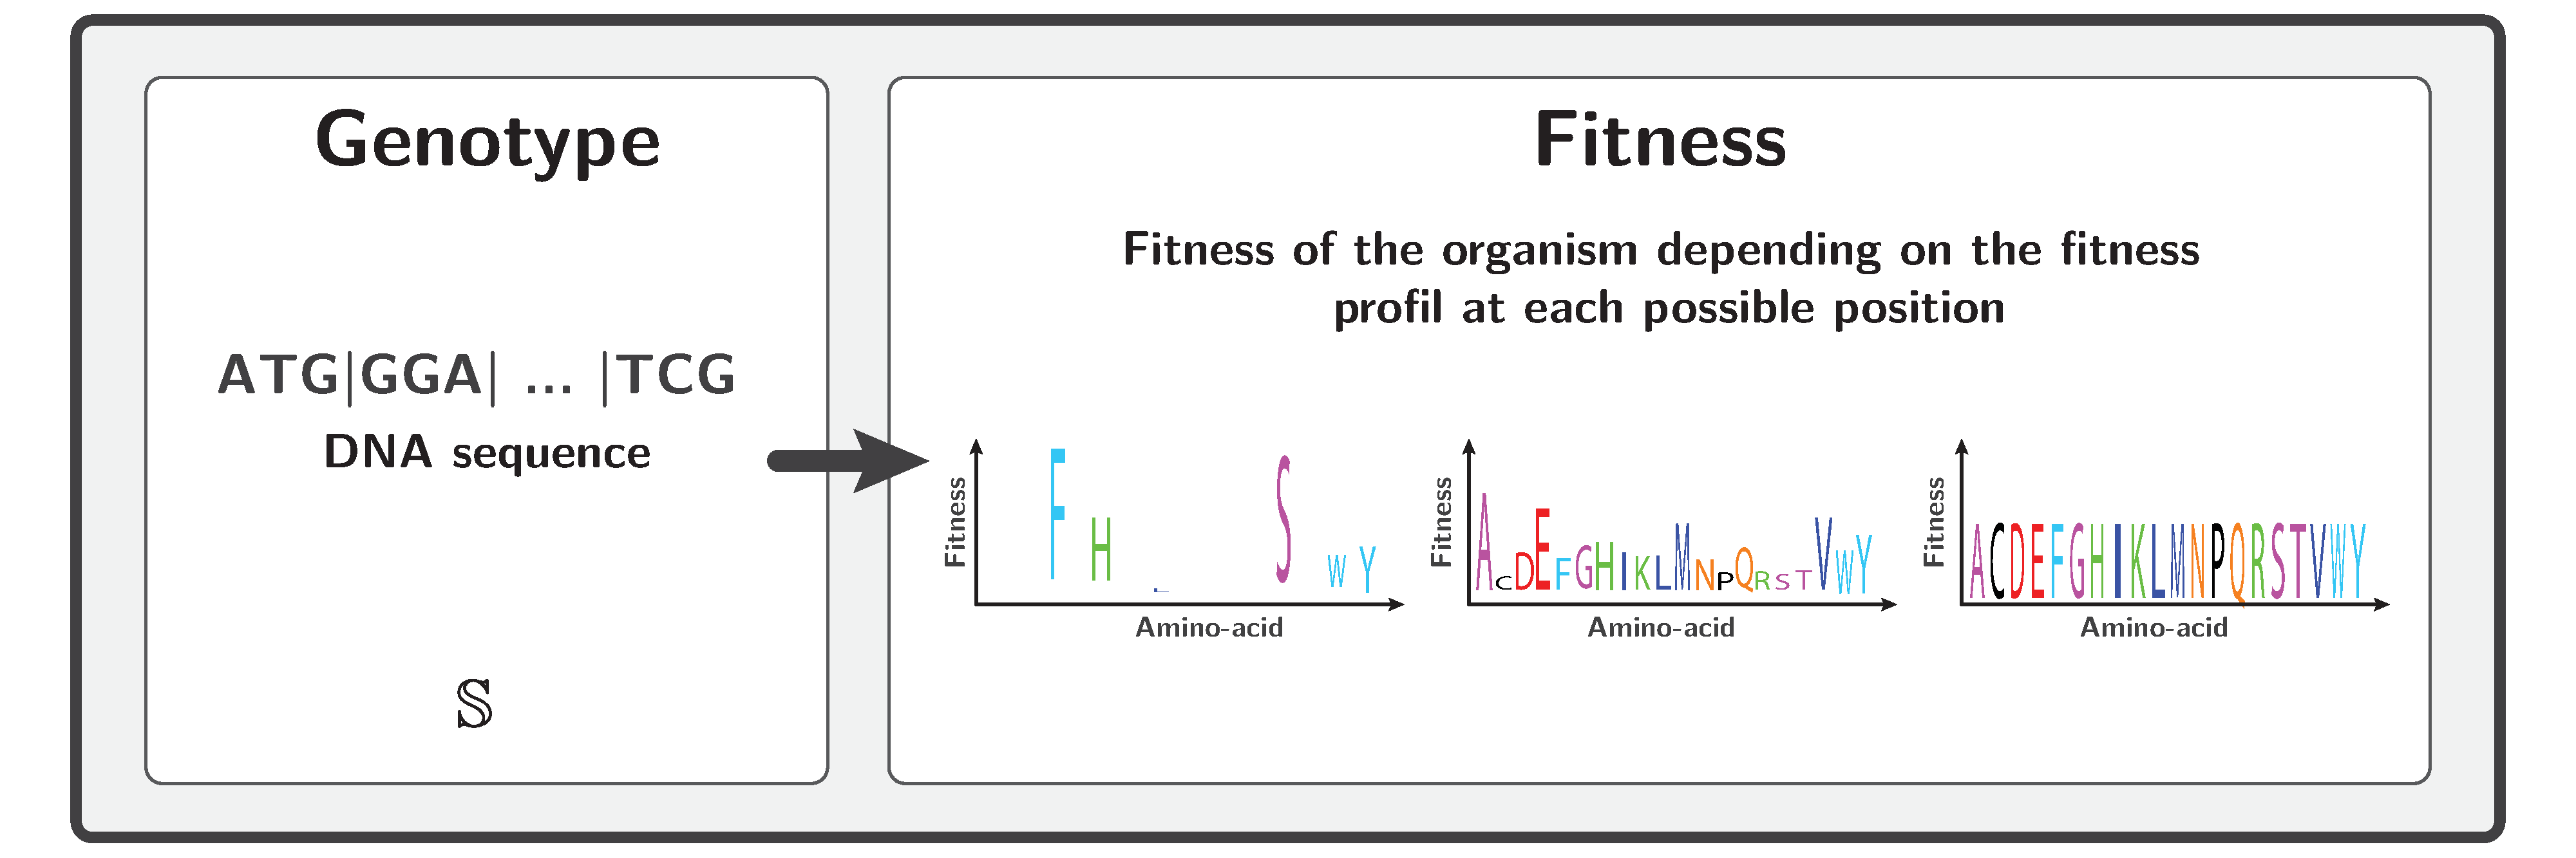
\includegraphics[width=\textwidth] {ModelSimuDiv}
	\end{center}

	The next change in the protein coding {DNA} and the time to next the event is chosen using Gillespie's algorithm~\citep{Gillespie1977}, according to the rates of {substitution} between codons:
	\begin{equation}
	{\submatrix_{\itoj}}
		= \mu_{\itoj} \dfrac{4 \Ne s \left( \Seqi^{t},\Seqi^{t+1}\right)}{{1 - \e^{-4 \Ne s \left( \Seqi^{t},\Seqi^{t+1}\right)} }},
	\end{equation}
	where ${\submatrix_{\itoj}} = \mu_{\itoj}$ in the case of {synonymous} substitutions.


	\begin{figure}[H]
		\centering
		\begin{minipage}{0.32\linewidth}
			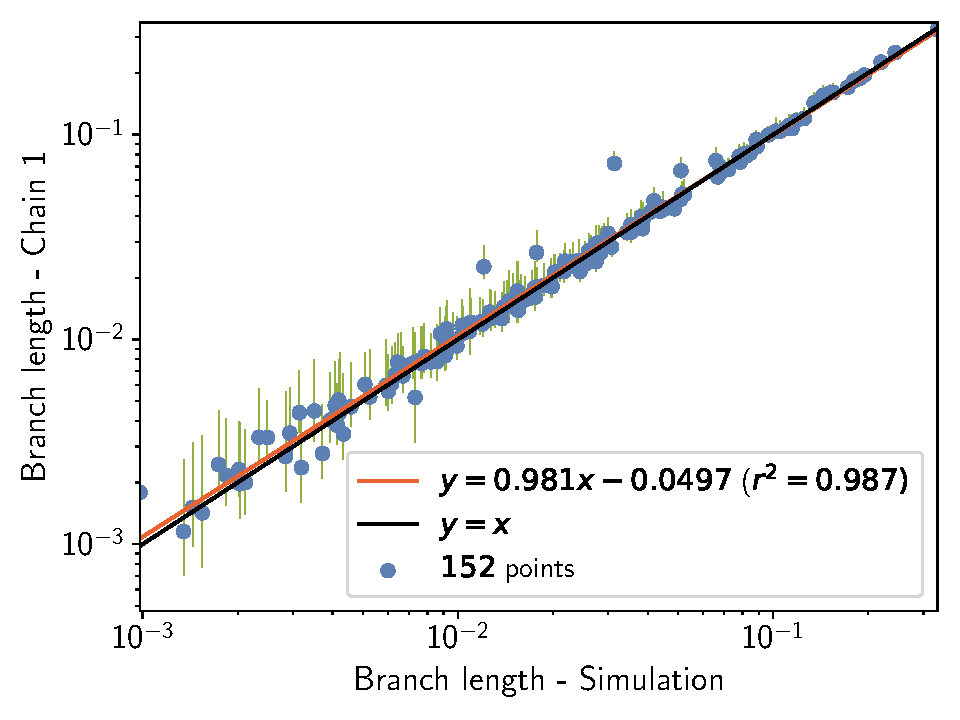
\includegraphics[width=\linewidth, page=1]{simulations/BranchWise_SimuDiv_SiteMutSelBranchNe_BranchCorrelation_Log10BranchLength}
		\end{minipage} \hfill
		\begin{minipage}{0.32\linewidth}
			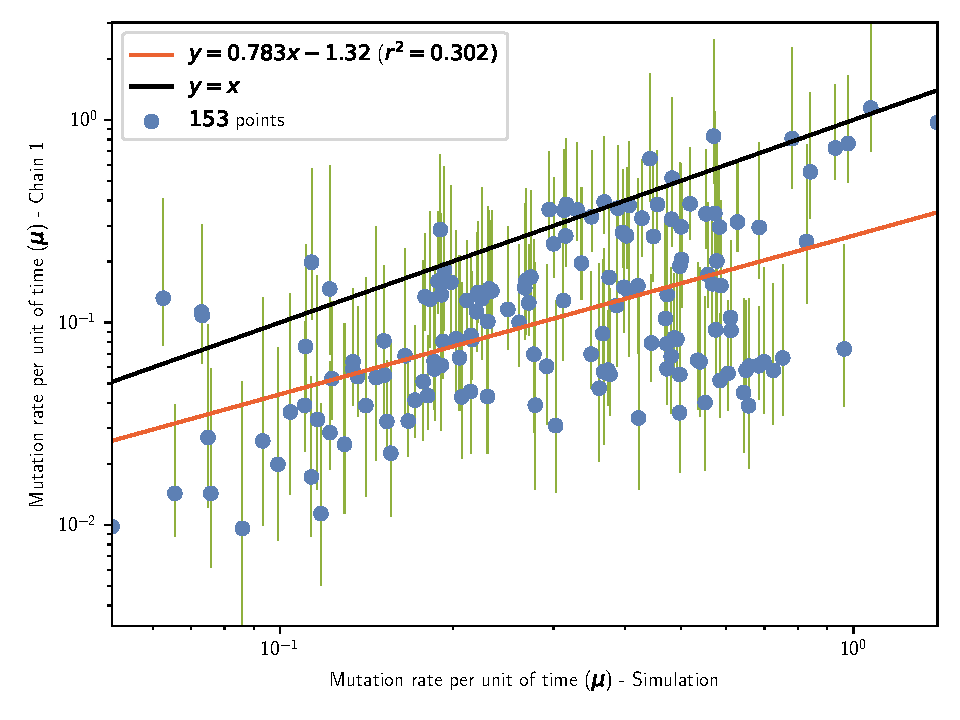
\includegraphics[width=\linewidth, page=1]{simulations/BranchWise_SimuDiv_SiteMutSelBranchNe_BranchCorrelation_LogMutationRatePerTime}
		\end{minipage} \hfill
		\begin{minipage}{0.32\linewidth}
			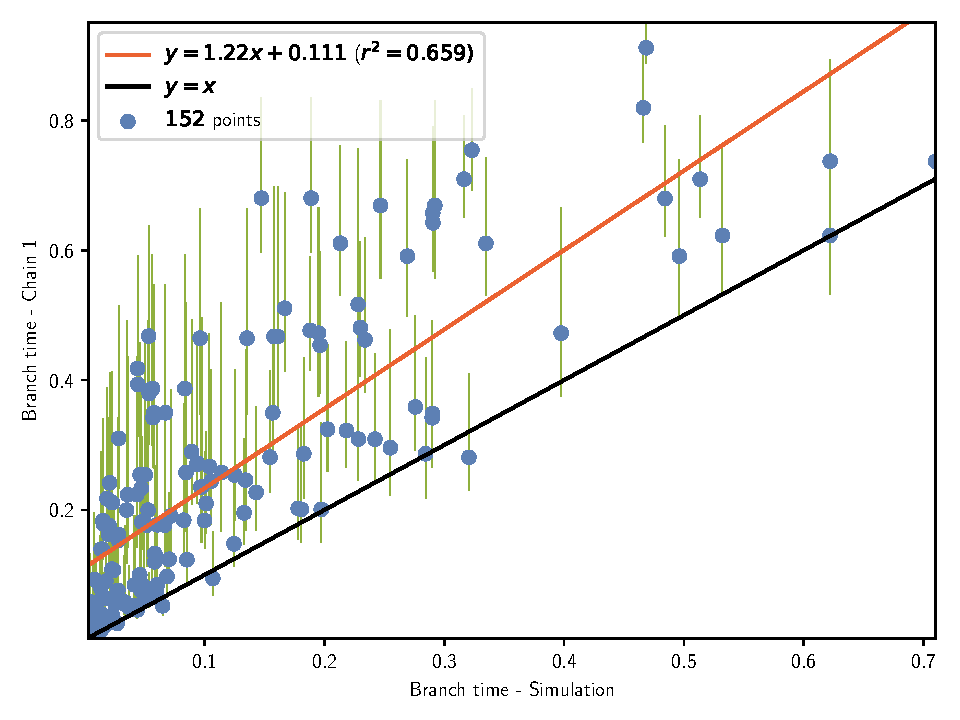
\includegraphics[width=\linewidth, page=1]{simulations/BranchWise_SimuDiv_SiteMutSelBranchNe_BranchCorrelation_BranchTime}
		\end{minipage} \hfill
		\begin{minipage}{0.32\linewidth}
			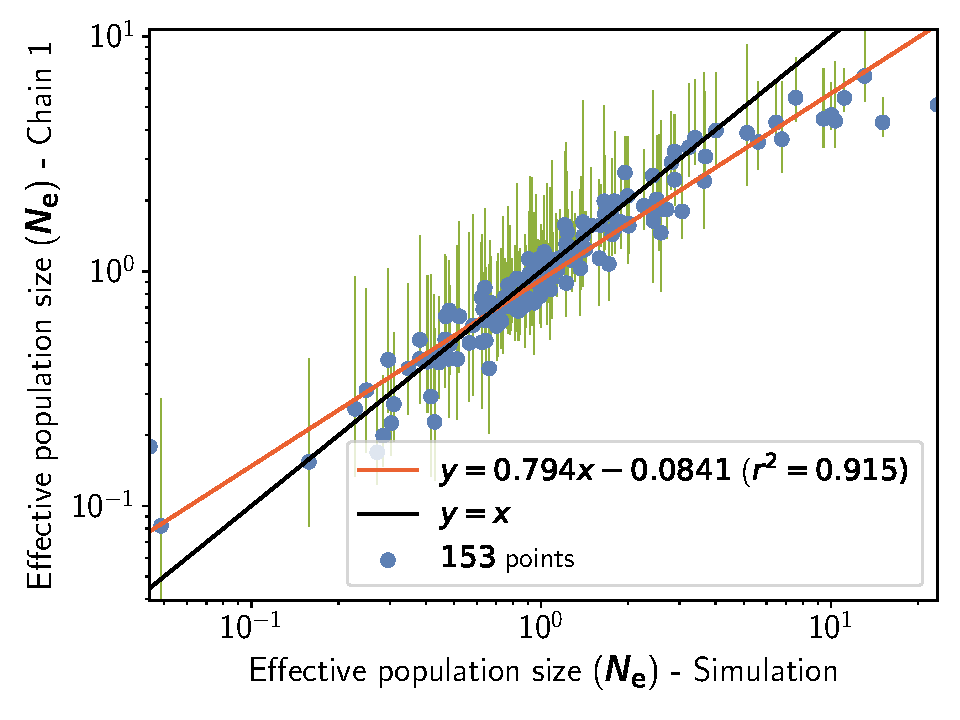
\includegraphics[width=\linewidth, page=1]{simulations/BranchWise_SimuDiv_SiteMutSelBranchNe_BranchCorrelation_LogPopulationSize}
		\end{minipage}
		\begin{minipage}{0.32\linewidth}
			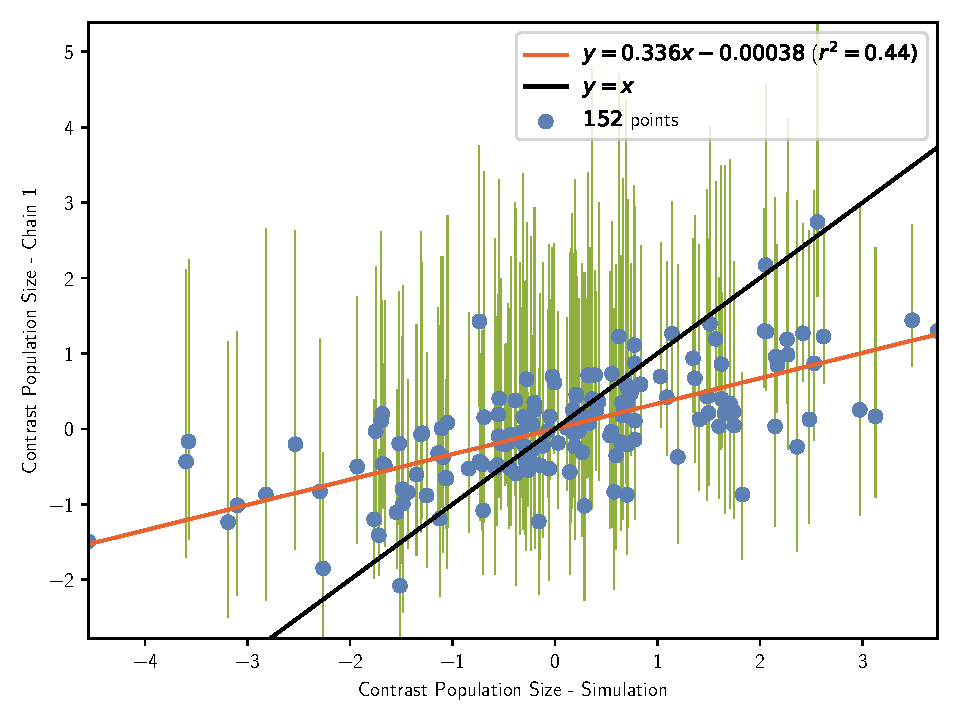
\includegraphics[width=\linewidth, page=1]{simulations/BranchWise_SimuDiv_SiteMutSelBranchNe_BranchCorrelation_ContrastPopulationSize}
		\end{minipage} \hfill
		\caption[Inferred branch parameters for \texttt{SimuDiv}]{
		Inferred branch parameters under simulations accounting for site-specific amino-acid profiles, long term fluctuation of $\Ne$, mutation rate per generation and generation time.
		Estimation is obtained with the mechanistic inference model developed in this paper of site-specific amino-acid fitness profiles and log-Brownian process for $\Ne$, $\mu$ and life-history traits.
		}
	\end{figure}


	\begin{figure}[H]
		\centering
		\begin{minipage}{0.49\linewidth}
			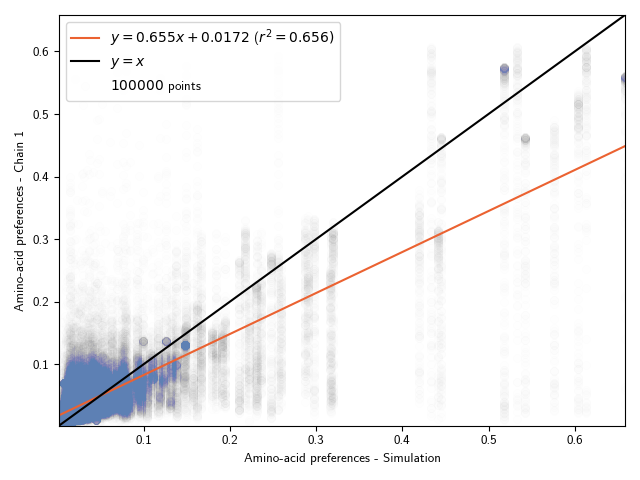
\includegraphics[width=\linewidth, page=1]{simulations/BranchWise_SimuDiv_SiteMutSelBranchNe_ProfileCorrelation.png}
		\end{minipage} \hfill
		\begin{minipage}{0.49\linewidth}
			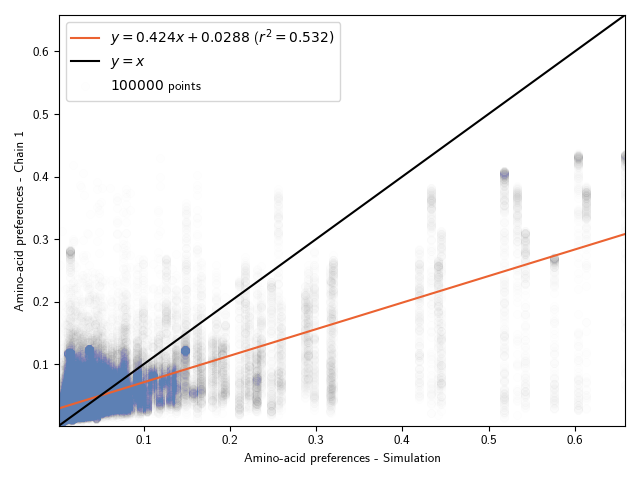
\includegraphics[width=\linewidth, page=1]{simulations/BranchWise_SimuDiv_SiteMutSel_ProfileCorrelation.png}
		\end{minipage}
		\caption[Inferred site amino-acid profiles for \texttt{SimuDiv}]{
		Inferred and simulated site-specific amino-acid profiles under simulation accounting for long term fluctuation of $\Ne$, mutation rate per generation and generation time.
		Estimation is obtained with the mechanistic inference model developed in this paper of site-specific amino-acid fitness profiles and log-Brownian process for $\Ne$, $\mu$ and life-history traits (in the left panel), or under the assumption of constant $\Ne$ (in the right panel).
		}
	\end{figure}

	\begin{table}[H]
		\centering
		\noindent\adjustbox{max width=\textwidth}{%
		\begin{tabu}{|c|c|c|}
			\hline
			\textbf{Experiment} & $\left\langle \entropy \right\rangle$ (\textbf{branch} $\Ne$) & $\left\langle \entropy \right\rangle$ (\textbf{constant} $\Ne$) \\ \hline
			\hline
			\texttt{SimuDiv}, chain~1 & $2.30 \pm 0.04$ & $2.45 \pm 0.02$\\ \hline
			\texttt{SimuDiv}, chain 2 & $2.30 \pm 0.04$ & $2.45 \pm 0.02$\\ \hline
		\end{tabu}}
		\caption[Inferred amino-acids entropy for \texttt{SimuDiv}]{
		Estimated amino-acid entropy under simulations accounting for long term fluctuation of $\Ne$, mutation rate per generation and generation time.
		Estimation is obtained with the mechanistic inference model developed in this paper of site-specific amino-acid fitness profiles and log-Brownian process for $\Ne$, $\mu$ and life-history traits (in the left column), or under the assumption of constant $\Ne$ (in the right column).
		}
	\end{table}

	\subsection{Wright-Fisher with polymorphism (\texttt{SimuPoly})}
	\label{subsec:wright-fisher-with-polymorphism}

	The evolutionary dynamics was formalized as a Wright-Fisher model with mutation, selection and drift
	The population is assumed to be panmictic, with {effective population size} $\Ne$ and with non-overlapping generations.

	\begin{center}
		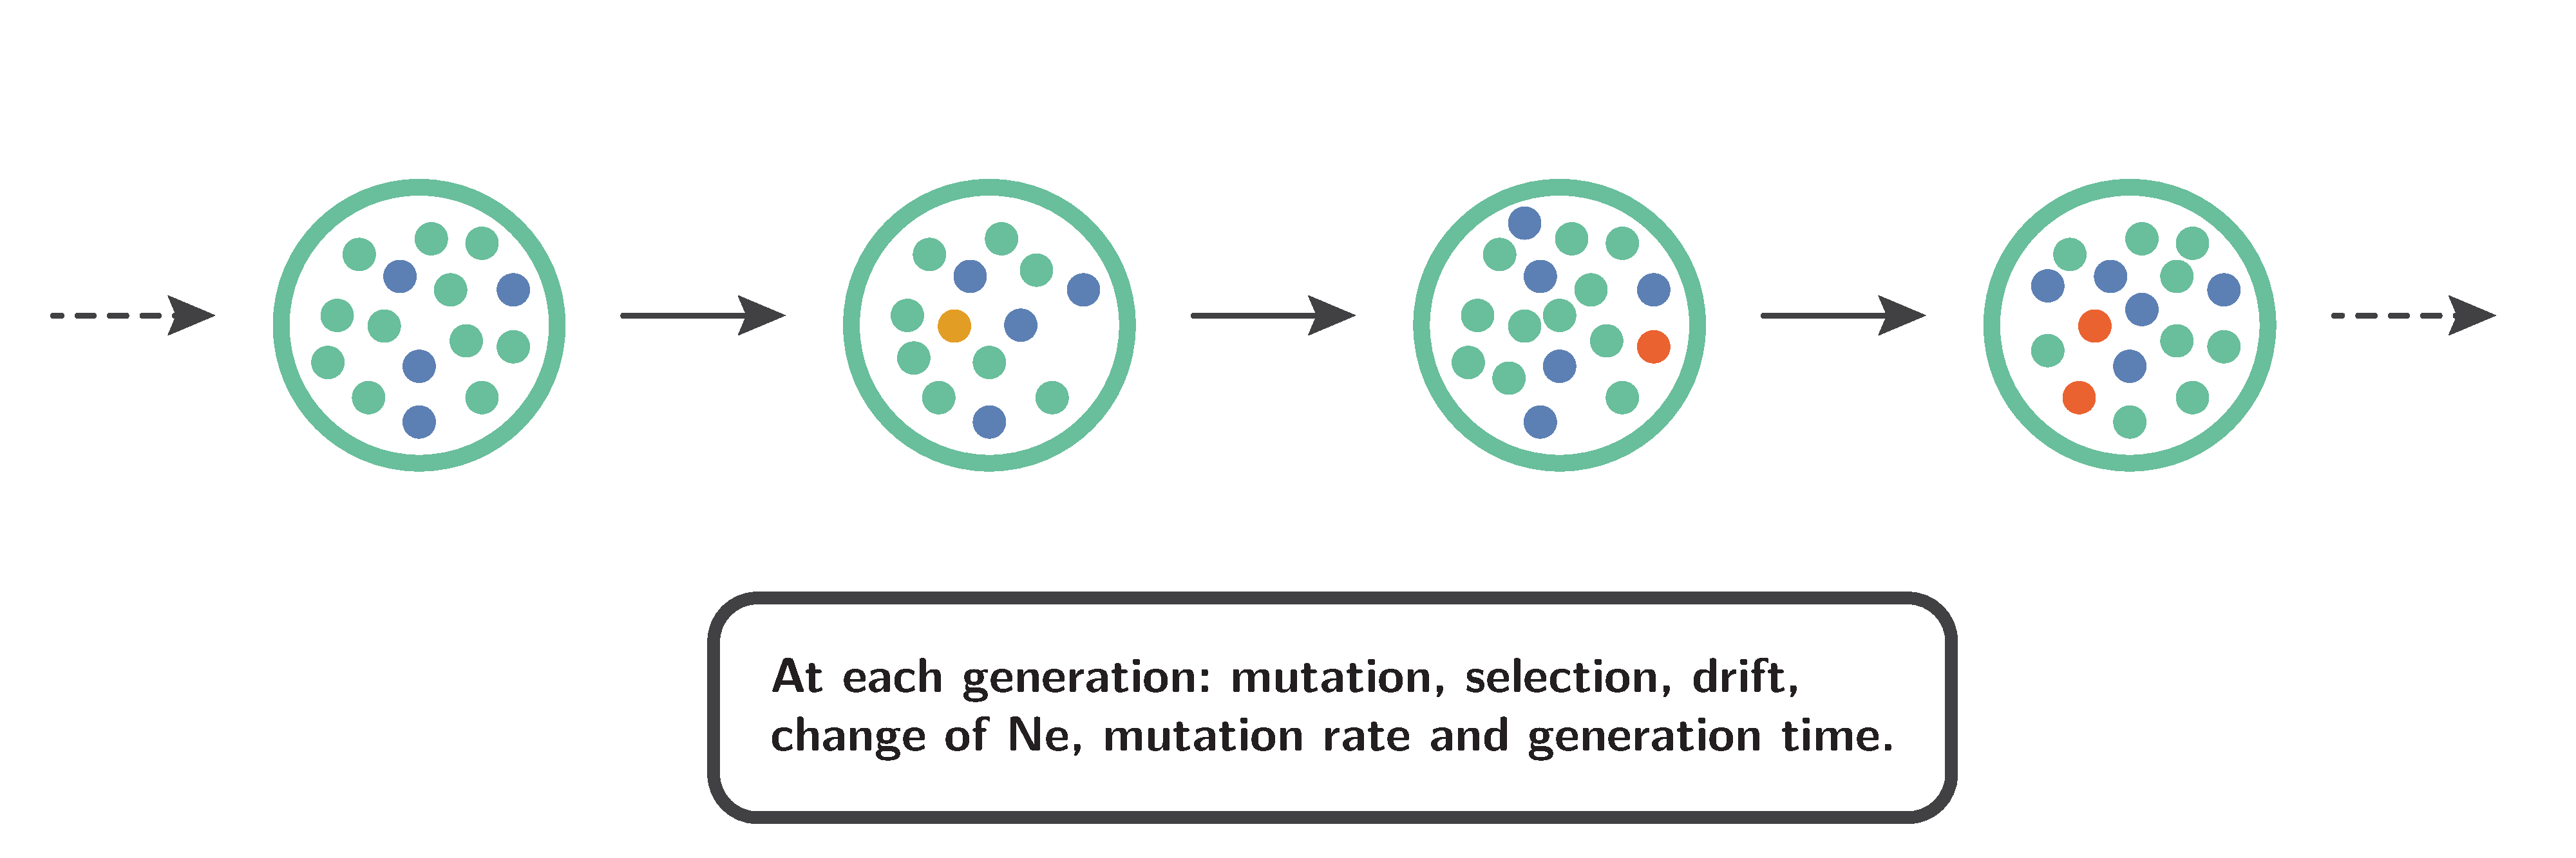
\includegraphics[width=\textwidth] {ModelSimuPoly}
	\end{center}

	\begin{figure}[H]
		\centering
		\begin{minipage}{0.32\linewidth}
			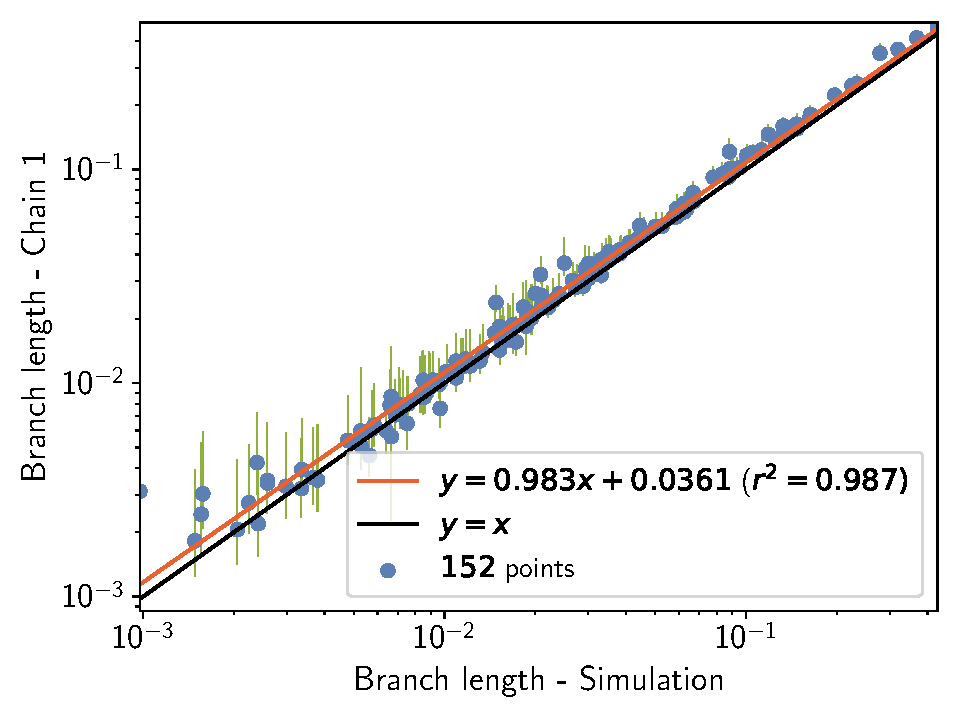
\includegraphics[width=\linewidth, page=1]{simulations/SimuPoly_SiteMutSelBranchNe_BranchCorrelation_Log10BranchLength}
		\end{minipage} \hfill
		\begin{minipage}{0.32\linewidth}
			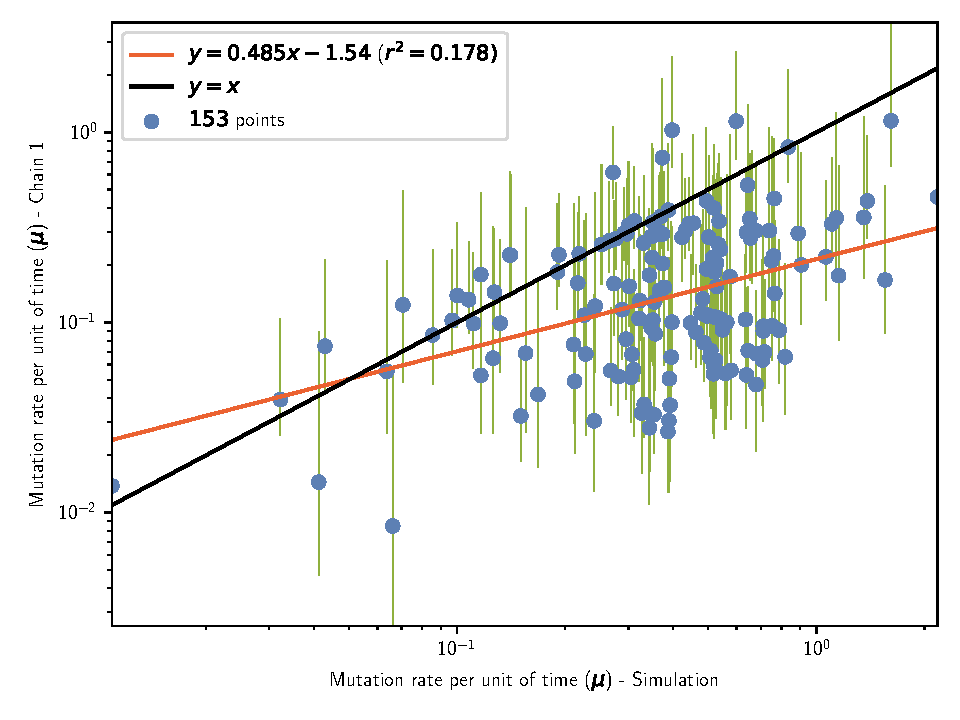
\includegraphics[width=\linewidth, page=1]{simulations/SimuPoly_SiteMutSelBranchNe_BranchCorrelation_LogMutationRatePerTime}
		\end{minipage} \hfill
		\begin{minipage}{0.32\linewidth}
			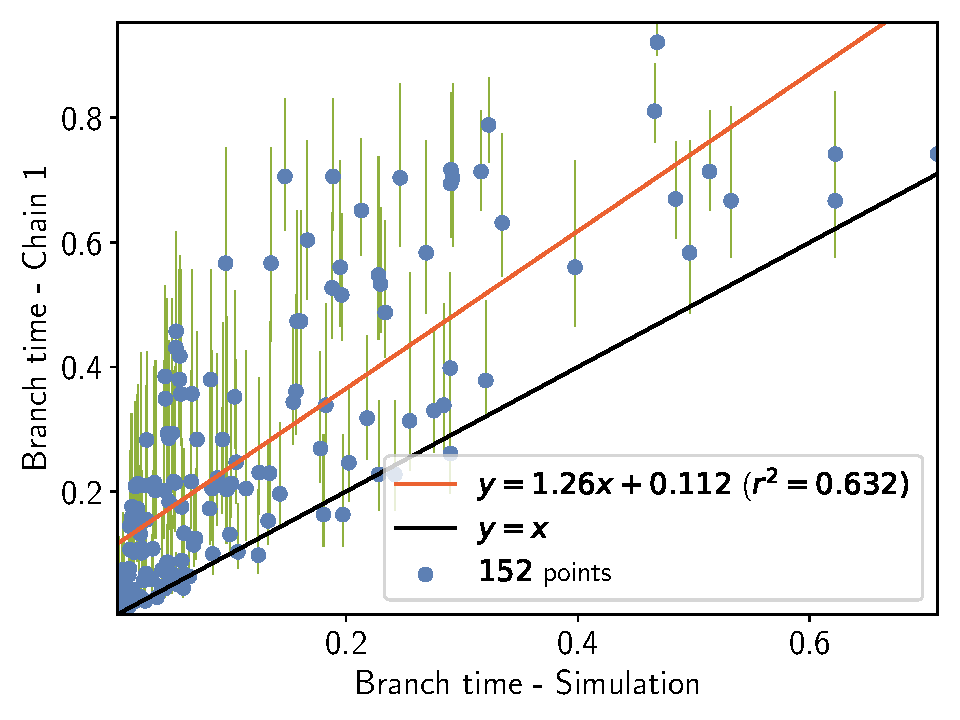
\includegraphics[width=\linewidth, page=1]{simulations/SimuPoly_SiteMutSelBranchNe_BranchCorrelation_BranchTime}
		\end{minipage} \hfill
		\begin{minipage}{0.32\linewidth}
			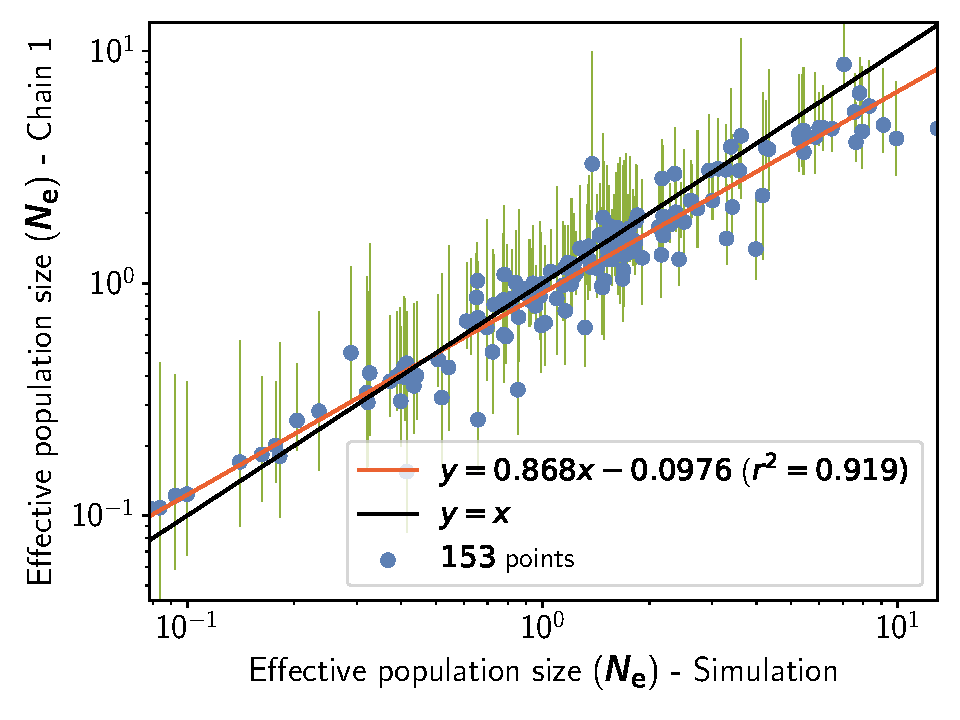
\includegraphics[width=\linewidth, page=1]{simulations/SimuPoly_SiteMutSelBranchNe_BranchCorrelation_LogPopulationSize}
		\end{minipage}
		\begin{minipage}{0.32\linewidth}
			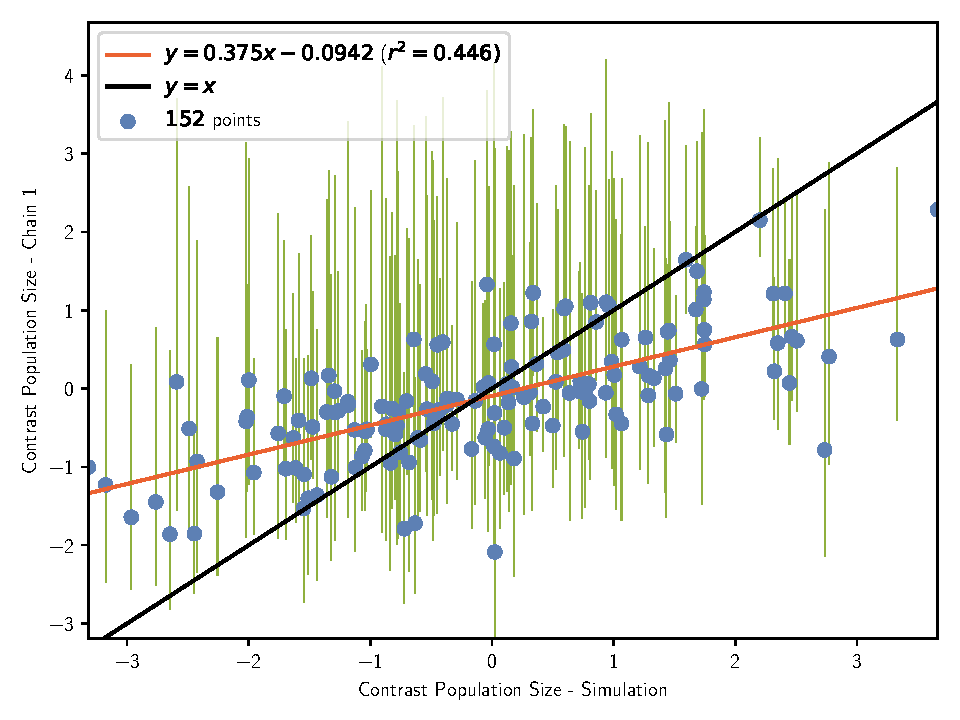
\includegraphics[width=\linewidth, page=1]{simulations/SimuPoly_SiteMutSelBranchNe_BranchCorrelation_ContrastPopulationSize}
		\end{minipage} \hfill
		\caption[Inferred branch parameters for \texttt{SimuPoly}]{
		Inferred branch parameters under simulation accounting for finite population effects, site linkage and short term fluctuation of $\Ne$.
		Estimation is obtained with the mechanistic inference model developed in this paper of site-specific amino-acid fitness profiles and log-Brownian process for $\Ne$, $\mu$ and life-history traits.
		}
	\end{figure}


	\begin{figure}[H]
		\centering
		\begin{minipage}{0.49\linewidth}
			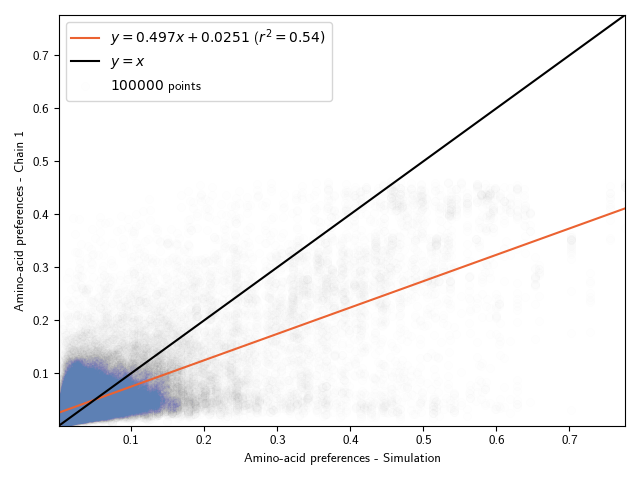
\includegraphics[width=\linewidth, page=1]{simulations/SimuPoly_SiteMutSelBranchNe_ProfileCorrelation.png}
		\end{minipage} \hfill
		\begin{minipage}{0.49\linewidth}
			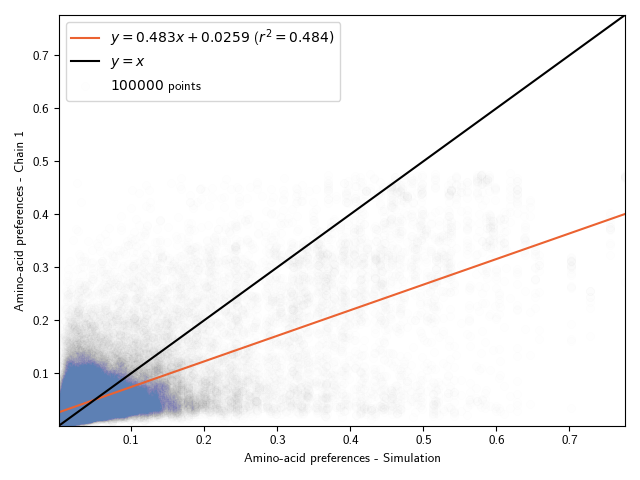
\includegraphics[width=\linewidth, page=1]{simulations/SimuPoly_SiteMutSel_ProfileCorrelation.png}
		\end{minipage}
		\caption[Inferred site amino-acid profiles for \texttt{SimuPoly}]{
		Inferred and simulated site-specific amino-acid profiles under simulation accounting for finite population effects, site linkage and short term fluctuation of $\Ne$.
		Estimation is obtained with the mechanistic inference model developed in this paper of site-specific amino-acid fitness profiles and log-Brownian process for $\Ne$, $\mu$ and life-history traits (in the left panel), or under the assumption of constant $\Ne$ (in the right panel).}
	\end{figure}

	\begin{table}[H]
		\centering
		\noindent\adjustbox{max width=\textwidth}{%
		\begin{tabu}{|c|c|c|}
			\hline
			\textbf{Experiment} & $\left\langle \entropy \right\rangle$ (\textbf{branch} $\Ne$) & $\left\langle \entropy \right\rangle$ (\textbf{constant} $\Ne$) \\ \hline
			\hline
			\texttt{SimuPoly}, chain~1 & $2.47 \pm 0.03$ & $2.37 \pm 0.02$\\ \hline
			\texttt{SimuPoly}, chain 2 & $2.47 \pm 0.03$ & $2.37 \pm 0.02$\\ \hline
		\end{tabu}}
		\caption[Inferred amino-acid entropy for \texttt{SimuPoly}]{
		Estimated amino-acid entropy under simulation accounting for finite population effects, site linkage and short term fluctuation of $\Ne$.
		Estimation is obtained with the mechanistic inference model developed in this paper of site-specific amino-acid fitness profiles and log-Brownian process for $\Ne$, $\mu$ and life-history traits (in the left column), or under the assumption of constant $\Ne$ (in the right column).}
	\end{table}

	\subsection{Fisher geometric landscape (\texttt{SimuGeo})}
	\label{subsec:fisher-geometric-landscape}

	We simulated substitutions in a protein using an adaptation of Fisher's geometric landscape~\citep{Tenaillon2014,Blanquart2016}.
	In the original context, the {phenotype} is a vector ($\phenoGeo$) in a multidimensional space, where the number of dimensions is often termed complexity.
	From a {phenotype}, the fitness is a monotonously decreasing function of the {phenotype} distance to $0$.
	The exact functional phenotype-fitness map depends on $2$ external parameters controlling for strength ($\alpha$) and epistasis ($\beta$).
	If the phenotype-fitness map is explicit, the genotype-phenotype map is more pervasive.
	Mutations are seen has displacement of the {phenotype} in the multidimensional space.
	Beneficial mutations are moving the {phenotype} closer to $0$, whereas deleterious mutations are moving the {phenotype} further away.
	In such original context, the distribution of mutational effects is not dependent on the current genotype, but this can be relaxed using a genotype-phenotype map.\\

	In a protein context, the genotype-phenotype map can be defined by assigning to each of the $20$ amino acid a vector in the multidimensional space.
	Since different sites of the protein do not have the same physico-chimical properties, we can define a specific genotype-phenotype map for each position of the sequence.
	Overall, the protein {phenotype} is computed as the sum of site-specific multidimensional vectors, obtained by accessing the amino acid present at each site of the protein.
	From a {DNA} sequence $\Seqi^t$ after $t$ substitutions, the protein's {phenotype} is given by:
	\begin{equation}
		\phenoGeo\left(\Seqi^{t}\right) = \sum\limits\sumSetsite \phenoGeo_{\site} \left(\Seqi^t(\site) \right),
	\end{equation}
	where $\phenoGeo_{\site}$ is the genotype-phenotype map at site $\site$.\\

	And the Wrightian fitness of $\Seqi^t$ is :
	\begin{equation}
		\wrightfit\left( \phenoGeo\left(\Seqi^{t}\right) \right) = e^{-\alpha \left| \phenoGeo\left(\Seqi^{t}\right) \right|^{\beta}},
	\end{equation}
	where strength ($\alpha > 0$) and epistasis ($\beta$) are parameters of the fitness function.
	\begin{center}
		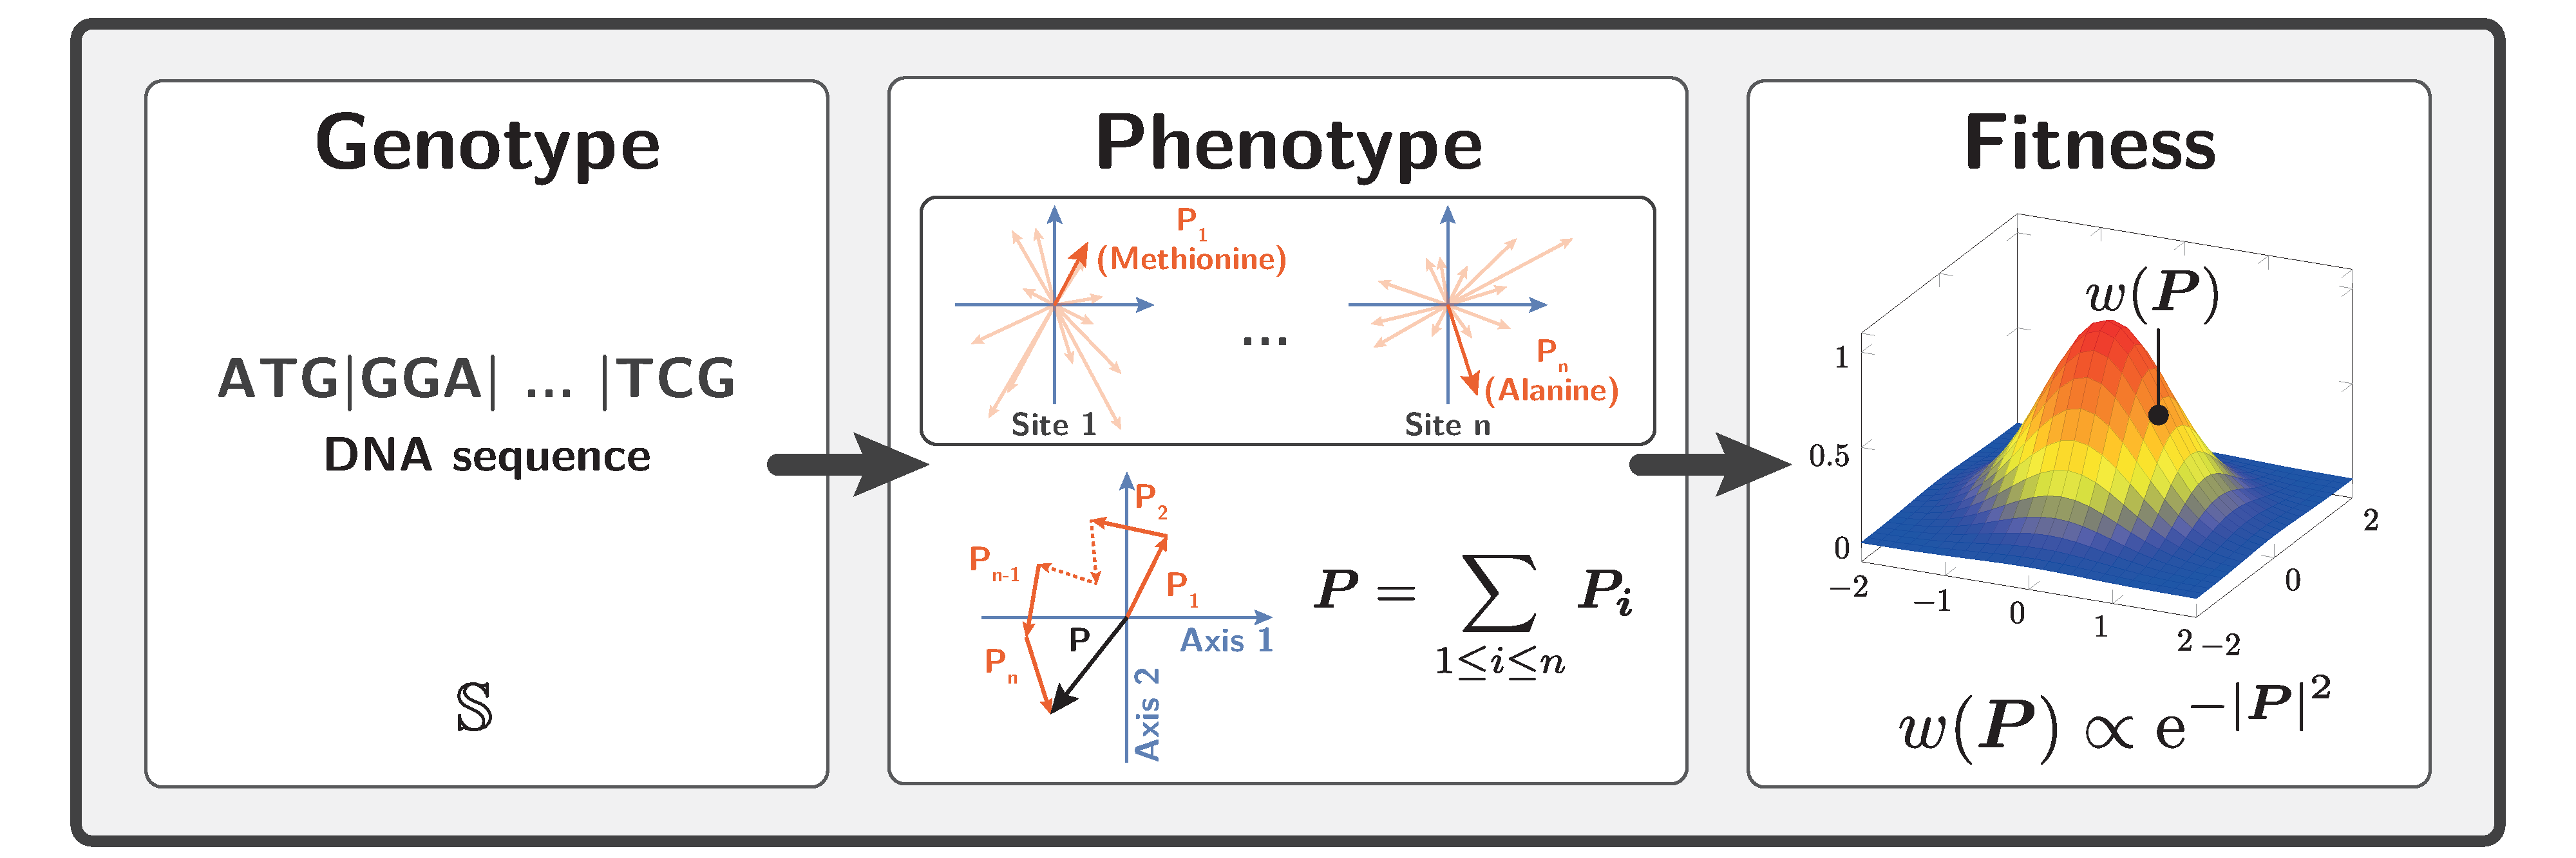
\includegraphics[width=\textwidth] {ModelSimuGeo}
	\end{center}
	For each possible mutant (at time $t+1$ substitutions), we compute $\phenoGeo\left(\Seqi^{t+1}\right)$ from the updated sequence $\Seqi^{t+1}$, and subsequently the selection coefficient of the mutant:
	\begin{equation}
		s \left( \Seqi^{t},\Seqi^{t+1}\right) = \dfrac{\wrightfit\left( \phenoGeo\left(\Seqi^{t+1}\right) \right) -\wrightfit\left( \phenoGeo\left(\Seqi^{t}\right) \right)}{\wrightfit\left( \phenoGeo\left(\Seqi^{t}\right) \right)}.
	\end{equation}
	The next change in the protein coding {DNA} and the time to next the event is chosen using Gillespie's algorithm~\citep{Gillespie1977}, according to the rates of {substitution} between codons:
	\begin{equation}
	{\submatrix_{\itoj}}
		= \mu_{\itoj} \dfrac{4 \Ne s \left( \Seqi^{t},\Seqi^{t+1}\right)}{{1 - \e^{-4 \Ne s \left( \Seqi^{t},\Seqi^{t+1}\right)} }},
	\end{equation}
	where ${\submatrix_{\itoj}} = \mu_{\itoj}$ in the case of {synonymous} substitutions.

	\begin{figure}[H]
		\centering
		\begin{minipage}{0.32\linewidth}
			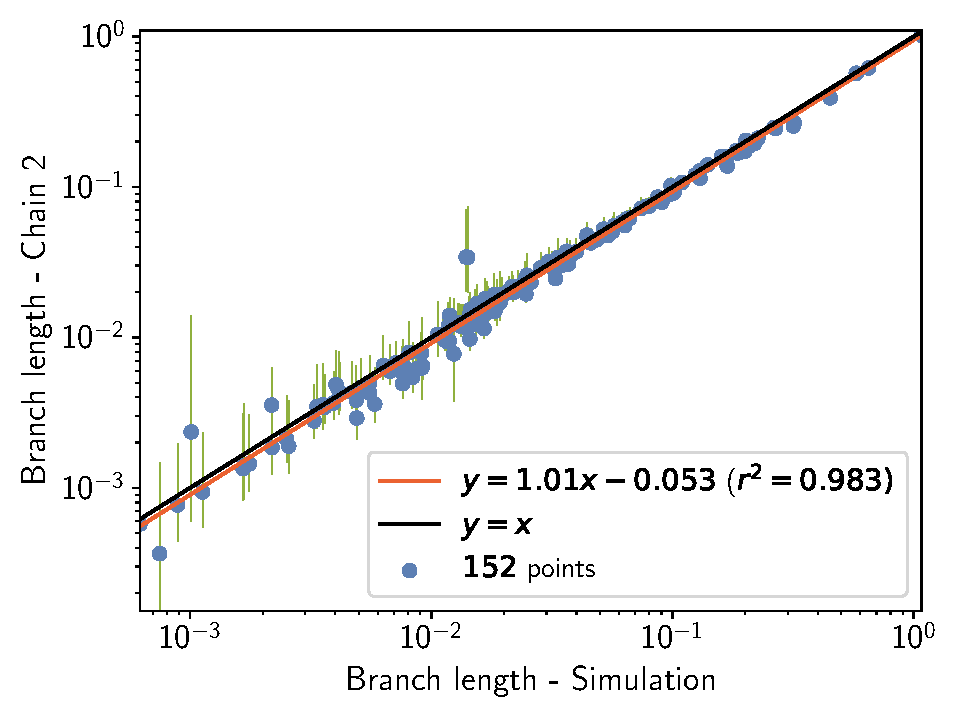
\includegraphics[width=\linewidth, page=1]{simulations/SimuGeo_SiteMutSelBranchNe_BranchCorrelation_Log10BranchLength}
		\end{minipage} \hfill
		\begin{minipage}{0.32\linewidth}
			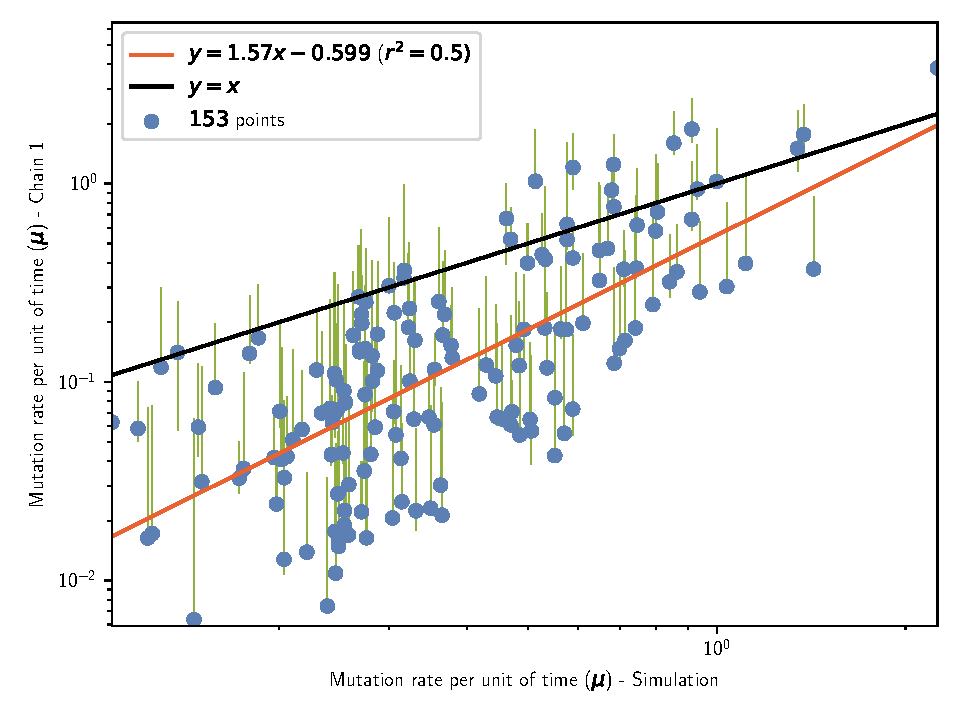
\includegraphics[width=\linewidth, page=1]{simulations/SimuGeo_SiteMutSelBranchNe_BranchCorrelation_LogMutationRatePerTime}
		\end{minipage} \hfill
		\begin{minipage}{0.32\linewidth}
			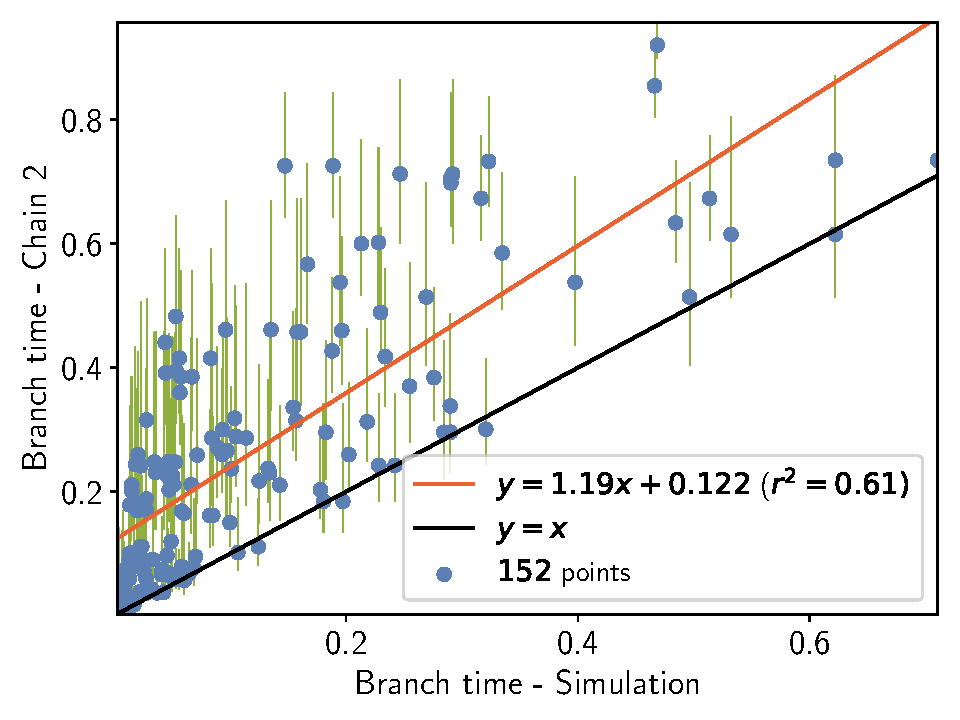
\includegraphics[width=\linewidth, page=1]{simulations/SimuGeo_SiteMutSelBranchNe_BranchCorrelation_BranchTime}
		\end{minipage} \hfill
		\begin{minipage}{0.32\linewidth}
			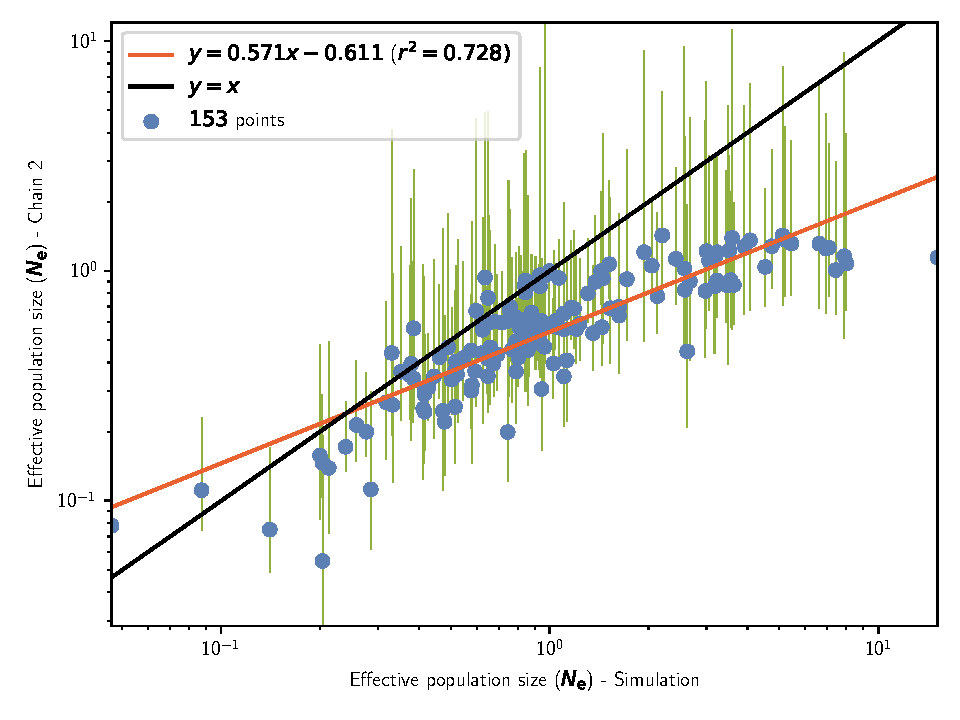
\includegraphics[width=\linewidth, page=1]{simulations/SimuGeo_SiteMutSelBranchNe_BranchCorrelation_LogPopulationSize}
		\end{minipage}
		\begin{minipage}{0.32\linewidth}
			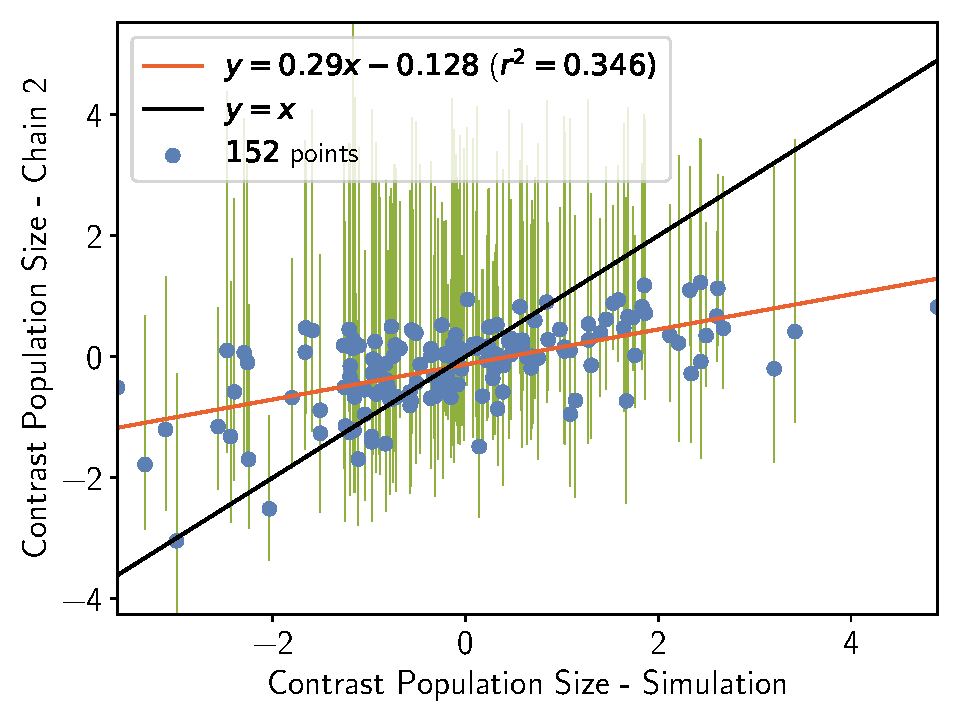
\includegraphics[width=\linewidth, page=1]{simulations/SimuGeo_SiteMutSelBranchNe_BranchCorrelation_ContrastPopulationSize}
		\end{minipage} \hfill
		\caption[Inferred branch parameters for \texttt{SimuGeo}]{
		Inferred branch parameters under simulation accounting for site epistasis in geometric landscape, thus fluctuation of the selection coefficient along the phylogeny.
		Estimation is obtained with the mechanistic inference model developed in this paper of site-specific amino-acid fitness profiles and log-Brownian process for $\Ne$, $\mu$ and life-history traits.
		}
	\end{figure}


	\begin{table}[H]
		\centering
		\noindent\adjustbox{max width=\textwidth}{%
		\begin{tabu}{|c|c|c|}
			\hline
			\textbf{Experiment} & $\left\langle \entropy \right\rangle$ (\textbf{branch} $\Ne$) & $\left\langle \entropy \right\rangle$ (\textbf{constant} $\Ne$) \\ \hline
			\hline
			\texttt{SimuGeo}, chain~1 & $2.27 \pm 0.02$ & $2.46 \pm 0.02$\\ \hline
			\texttt{SimuGeo}, chain 2 & $2.23 \pm 0.04$ & $2.46 \pm 0.02$\\ \hline
		\end{tabu}}
		\caption[Amino-acid entropy for \texttt{SimuGeo}]{
		Estimated amino-acid entropy under simulation accounting for site epistasis (geometric landscape), thus fluctuation of the selection coefficient along the phylogeny.
		Estimation is obtained with the mechanistic inference model developed in this paper of site-specific amino-acid fitness profiles and log-Brownian process for $\Ne$, $\mu$ and life-history traits (in the left column), or under the assumption of constant $\Ne$ (in the right column).
		}
	\end{table}

	\subsection{Protein folding probability (\texttt{SimuFold})}
	\label{subsec:protein-folding-probability}

	We simulated substitutions in the protein phosphatase ($\Nsite=300$ {codon} sites) as in \citet{Goldstein2017}.
	From a {DNA} sequence $\Seqi^t$ after $t$ substitutions, we compute the free energy of the folded state $ \GFold \left(\Seqi^{t}\right)$, using the 3-dimensional structure of the folded state and pair-wise contact energies between neighboring amino-acid residues:
	\begin{equation}
		\GFold \left(\Seqi^{t}\right) = \sum\limits\sumSetsite \sum\limits_{r \in \mathcal{V}(\site)} I \left(\Seqi^t(\site), \Seqi^t(r) \right),
	\end{equation}
	where $I(a,b)$ is the pair-wise contact energies between amino acid $a$ and $b$, using contact potentials estimated by \citet{Miyazawa1985}, and $\mathcal{V}(\site)$ are the neighbor residues of site $\site$ (closer than $7\angstrom$) in the 3D structure.\\

	The free energy of unfolded states $\GUnfold \left(\Seqi^{t}\right)$ is approximated using $55$ decoy 3D structures that supposedly represent a sample of possible unfolded states:
	\begin{equation}
		\GUnfold \left(\Seqi^{t}\right) = \left\langle G\left(\Seqi^{t}\right) \right\rangle - kT \ln (1.0\text{E}^{160}) - \dfrac{2 \left[ \left\langle G\left(\Seqi^{t}\right)^2 \right\rangle - \left\langle G\left(\Seqi^{t}\right) \right\rangle^2\right] }{kT}
	\end{equation}
	where the average $\left\langle . \right\rangle$ runs other the $55$ decoy 3D structures, and $k$ is the Boltzmann constant and $T$ the temperature in Kelvin.\\

	From the energy of folded and unfolded states, we can compute the difference in free energy between the states:
	\begin{equation}
		\phenoFold\left(\Seqi^{t}\right) = \GFold \left(\Seqi^{t}\right) - \GUnfold \left(\Seqi^{t}\right)
	\end{equation}

	Wrightian fitness is defined as the probability of our protein to be in the folded state:
	\begin{equation}
		\wrightfit \left( \phenoFold\left(\Seqi^{t}\right) \right) = \probaFold \left(\Seqi^{t}\right) = \dfrac{e^{-\beta \GFold \left(\Seqi^{t}\right) }}{e^{-\beta \GFold  \left(\Seqi^{t}\right) } + e^{-\beta \GUnfold \left(\Seqi^{t}\right) }} = \dfrac{1}{1 + e^{\beta \phenoFold\left(\Seqi^{t}\right) }},
	\end{equation}
	where $\beta$ is the inverse of the temperature ($\beta=1/kT$).
	\begin{center}
		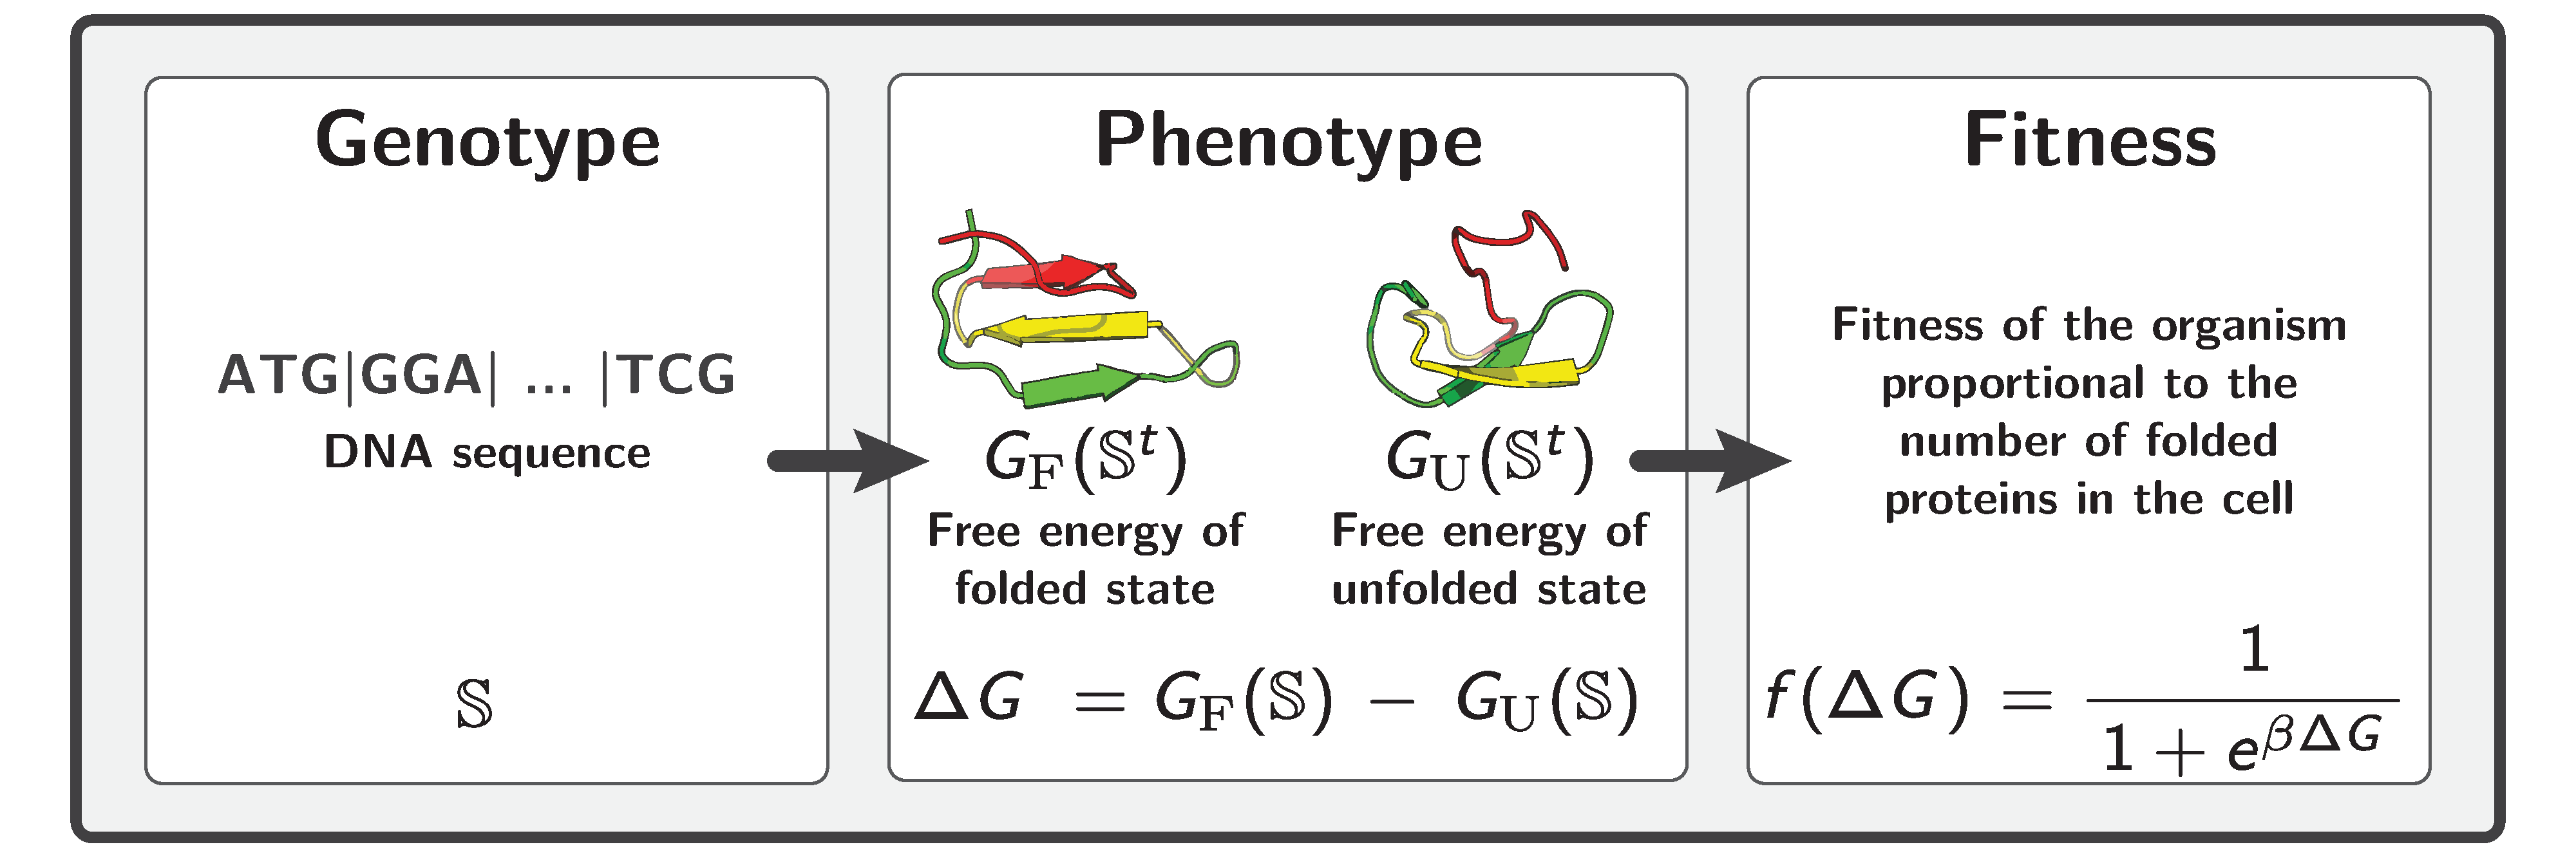
\includegraphics[width=\textwidth] {ModelSimuFold}
	\end{center}
	For each possible mutant (at time $t+1$ substitutions), we compute $\phenoFold^{t+1}$ from the updated sequence $\Seqi^{t+1}$, and subsequently the selection coefficient of the mutant:
	\begin{equation}
		s \left( \Seqi^{t},\Seqi^{t+1}\right) = \dfrac{\wrightfit\left( \phenoFold\left(\Seqi^{t+1}\right) \right) -\wrightfit\left( \phenoFold\left(\Seqi^{t}\right) \right)}{\wrightfit\left( \phenoFold\left(\Seqi^{t}\right) \right)}.
	\end{equation}
	The next change in the protein coding {DNA} and the time to next the event is chosen using Gillespie's algorithm~\citep{Gillespie1977}, according to the rates of {substitution} between codons:
	\begin{equation}
	{\submatrix_{\itoj}}
		= \mu_{\itoj} \dfrac{4 \Ne s \left( \Seqi^{t},\Seqi^{t+1}\right)}{{1 - \e^{-4 \Ne s \left( \Seqi^{t},\Seqi^{t+1}\right)} }},
	\end{equation}
	where ${\submatrix_{\itoj}} = \mu_{\itoj}$ in the case of {synonymous} substitutions.

	\begin{figure}[H]
		\centering
		\begin{minipage}{0.32\linewidth}
			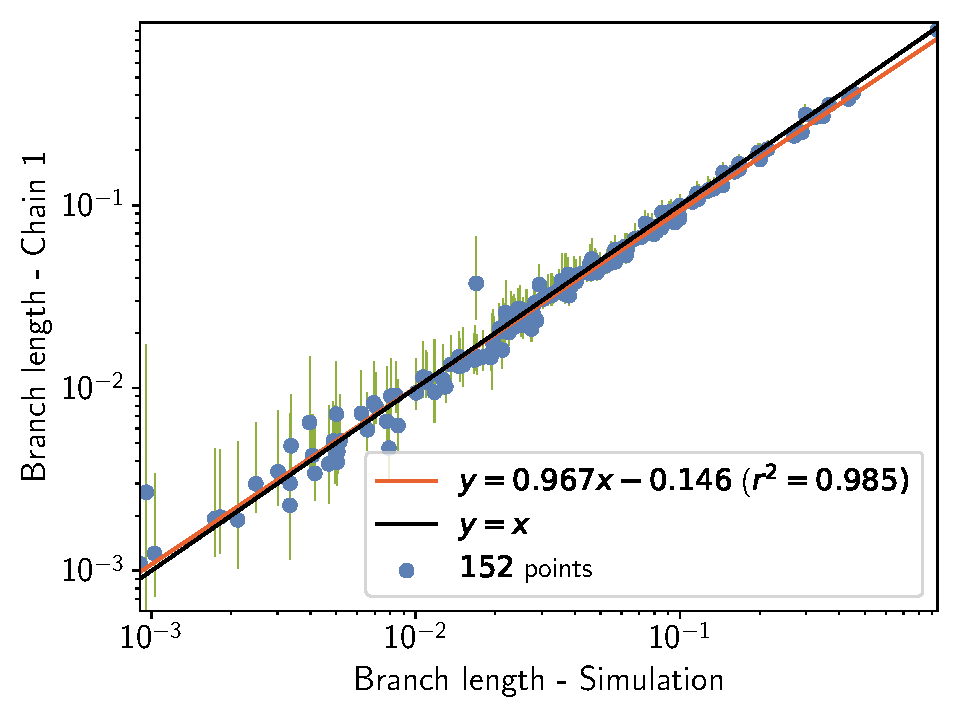
\includegraphics[width=\linewidth, page=1]{simulations/SimuFold_SiteMutSelBranchNe_BranchCorrelation_Log10BranchLength}
		\end{minipage} \hfill
		\begin{minipage}{0.32\linewidth}
			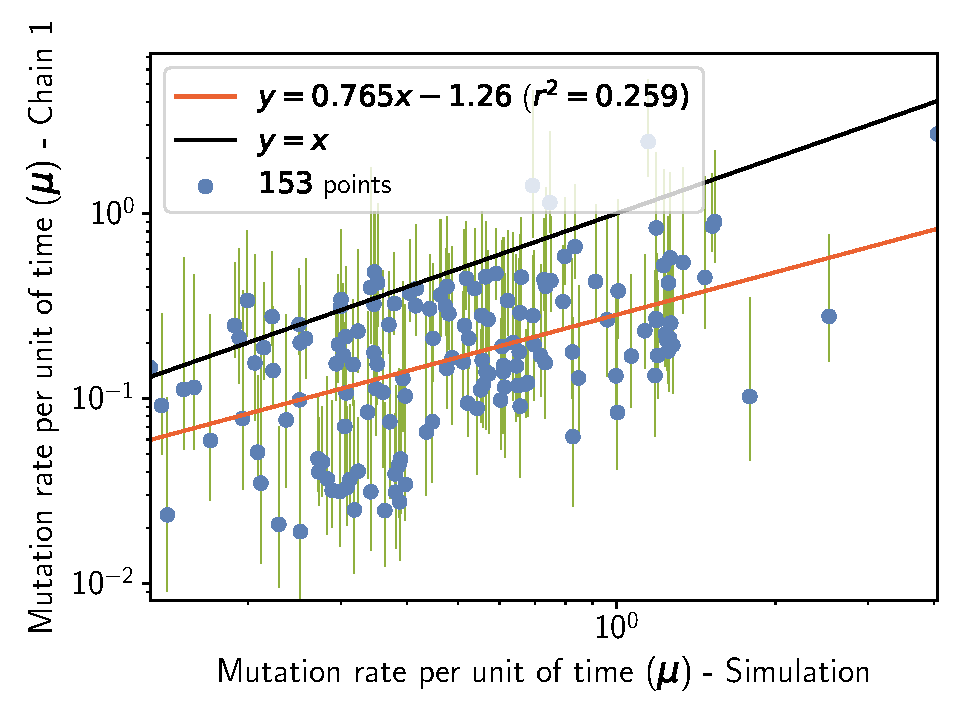
\includegraphics[width=\linewidth, page=1]{simulations/SimuFold_SiteMutSelBranchNe_BranchCorrelation_LogMutationRatePerTime}
		\end{minipage} \hfill
		\begin{minipage}{0.32\linewidth}
			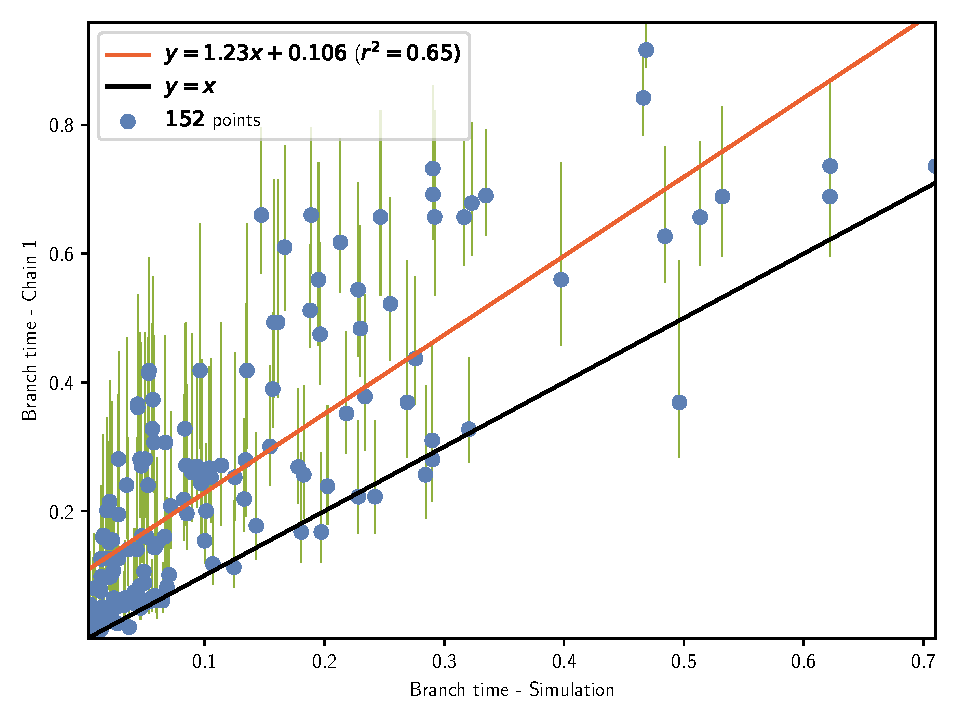
\includegraphics[width=\linewidth, page=1]{simulations/SimuFold_SiteMutSelBranchNe_BranchCorrelation_BranchTime}
		\end{minipage} \hfill
		\begin{minipage}{0.32\linewidth}
			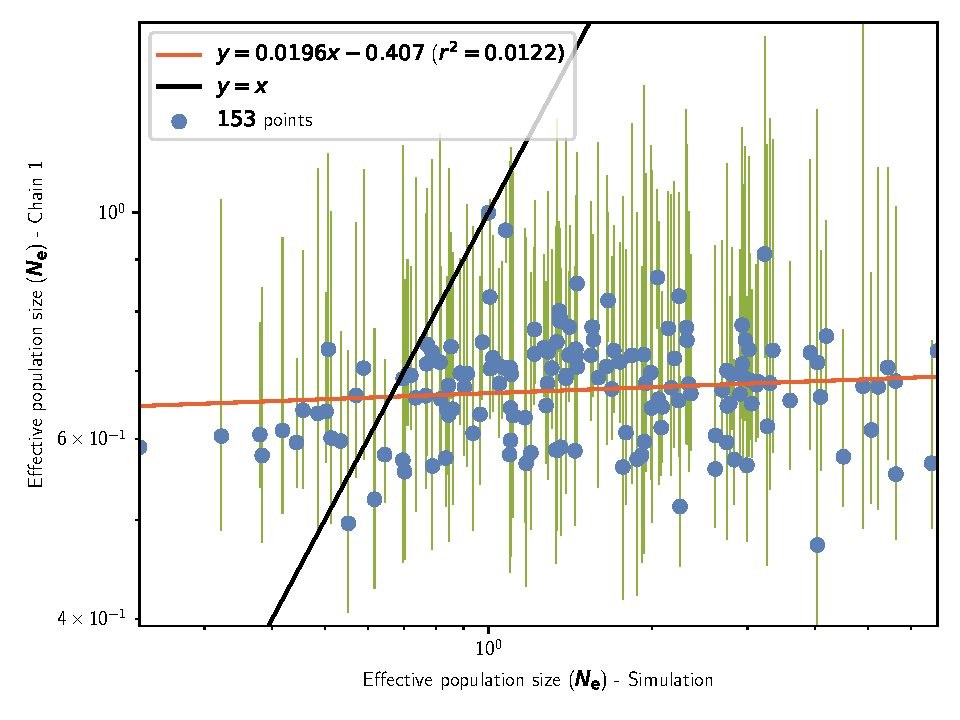
\includegraphics[width=\linewidth, page=1]{simulations/SimuFold_SiteMutSelBranchNe_BranchCorrelation_LogPopulationSize}
		\end{minipage}
		\begin{minipage}{0.32\linewidth}
			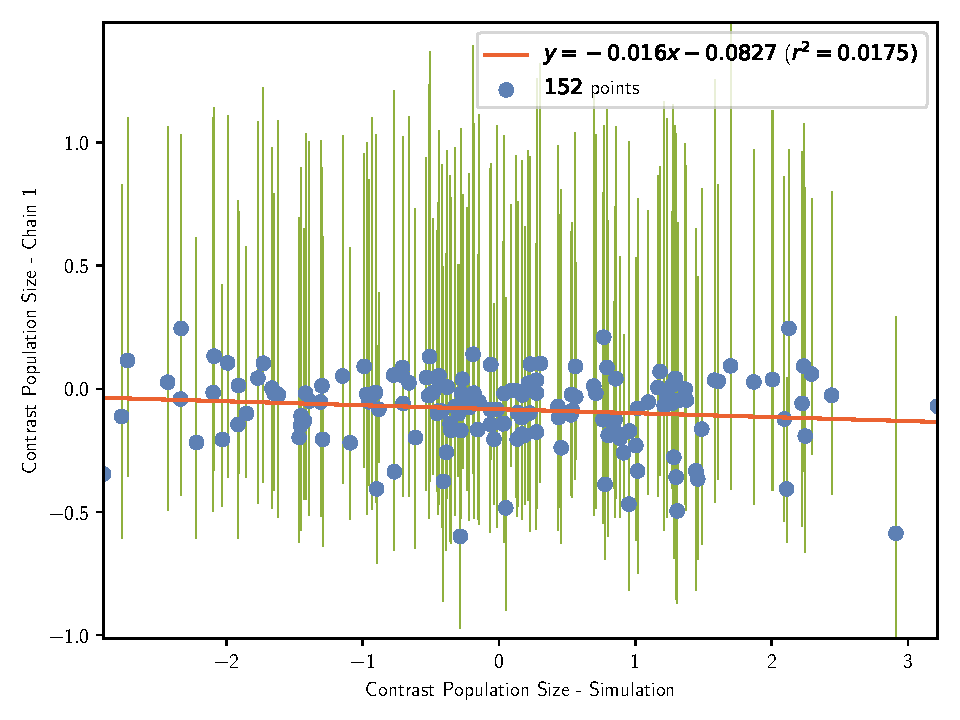
\includegraphics[width=\linewidth, page=1]{simulations/SimuFold_SiteMutSelBranchNe_BranchCorrelation_ContrastPopulationSize}
		\end{minipage} \hfill
		\caption[Inferred branch parameters for \texttt{SimuFold}]{
		Inferred branch parameters under simulation accounting for site epistasis (folding stability model), thus fluctuation of the selection coefficient along the phylogeny.
		Estimation is obtained with the mechanistic inference model developed in this paper of site-specific amino-acid fitness profiles and log-Brownian process for $\Ne$, $\mu$ and life-history traits.
		}
	\end{figure}

	\begin{table}[H]
		\centering
		\noindent\adjustbox{max width=\textwidth}{%
		\begin{tabu}{|c|c|c|}
			\hline
			\textbf{Experiment} & $\left\langle \entropy \right\rangle$ (\textbf{branch} $\Ne$) & $\left\langle \entropy \right\rangle$ (\textbf{constant} $\Ne$) \\ \hline
			\hline
			\texttt{SimuFold}, chain~1 & $1.31 \pm 0.05$ & $1.61 \pm 0.03$\\ \hline
			\texttt{SimuFold}, chain 2 & $1.30 \pm 0.04$ & $1.60 \pm 0.03$\\ \hline
		\end{tabu}}
		\caption[Amino-acid entropy in \texttt{SimuFold}]{
		Estimated amino-acid entropy under simulation accounting for site epistasis (folding stability model), thus fluctuation of the selection coefficient along the phylogeny.
		Obtained with the mechanistic inference model developed in this paper of site-specific amino-acid fitness profiles and log-Brownian process for $\Ne$, $\mu$ and life-history traits (in the left column), or under the assumption of constant $\Ne$ (in the right column).}
	\end{table}


	\section{Empirical data in mammals}
	\label{sec:empirical-data-in-mammals}

	\subsection{Chain convergence}
	\label{subsec:chain-convergence}
	Obtained with the mechanistic inference model developed in this paper of site-specific amino-acid fitness profiles and log-Brownian process for $\Ne$, $\mu$ and life-history traits.

	\begin{figure}[H]
		\centering
		\begin{minipage}{0.49\linewidth}
			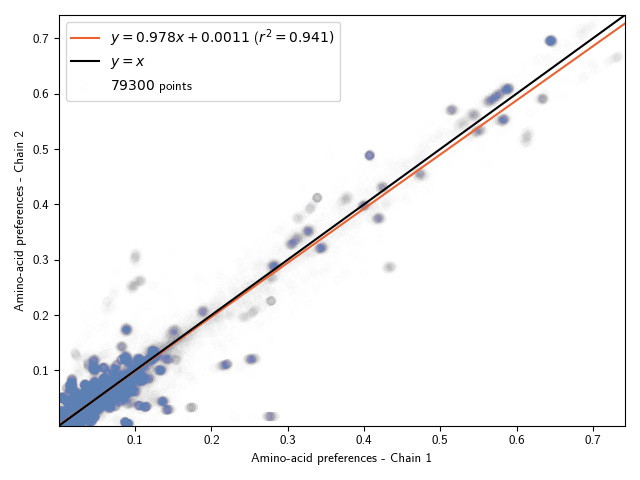
\includegraphics[width=\linewidth, page=1]{mammals/18CDS_SiteMutSelBranchNe_R1_ProfileCorrelation.png}
		\end{minipage} \hfill
		\begin{minipage}{0.49\linewidth}
			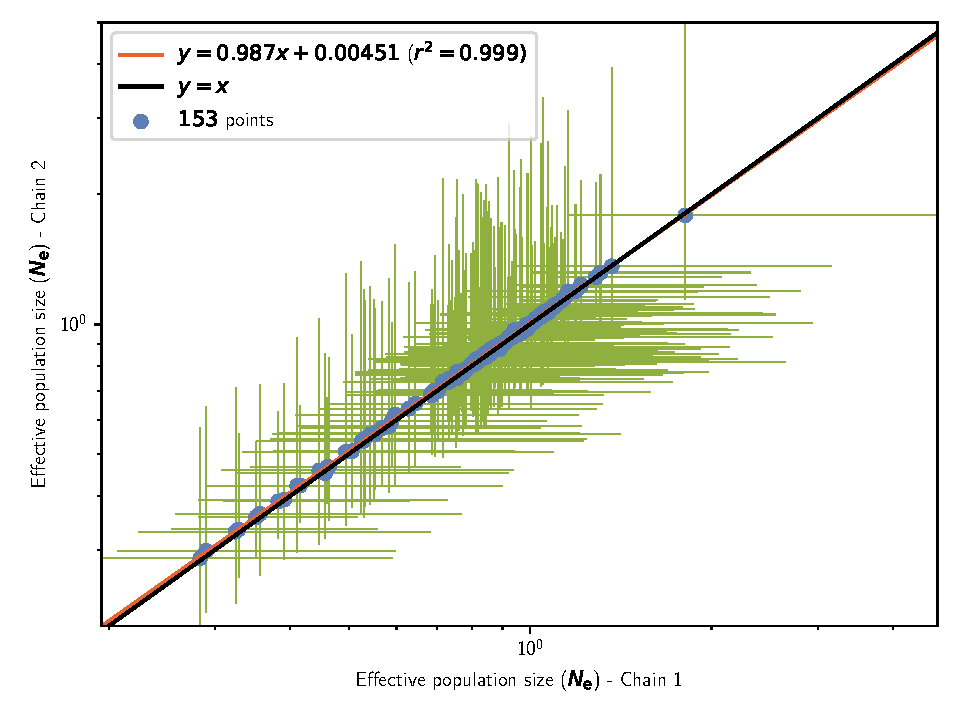
\includegraphics[width=\linewidth, page=1]{mammals/18CDS_SiteMutSelBranchNe_R1_LogPopulationSizeCorrelation}
		\end{minipage}
		\caption[Chain convergence of site profiles and branche $\Ne$]{
		Chain convergence of site amino-acid preferences (left panel) and branch $\Ne$ (right panel).}
	\end{figure}

	\subsection{Traits estimation \& correlation (replicate~1, chain~1)}
	Obtained with the mechanistic inference model developed in this paper of site-specific amino-acid fitness profiles and log-Brownian process for $\Ne$, $\mu$ and life-history traits.

	\begin{table}[H]
		\centering
\noindent\adjustbox{max width=\textwidth}{%
\begin{tabu}{|c||c|c|c|c|c|}
\hline
\textbf{Covariance ($\bm{\Sigma}$)} & $\bm{N_{\text{e}}}$ & $\bm{\mu}$ & \textbf{Maximum longevity } & \textbf{Adult weight } & \textbf{Female maturity }\\
\hhline{|=#=|=|=|=|=|}
$\bm{N_{\text{e}}}$ & $0.281^{**}$ & $0.324^{**}$ & $-0.268^{**}$ & $-1.29^{**}$ & $-0.308^{**}$\\\hline
$\bm{\mu}$ & - & $1.93^{**}$ & $-1.12^{**}$ & $-5.19^{**}$ & $-1.43^{**}$\\\hline
\textbf{Maximum longevity } & - & - & $0.934^{**}$ & $3.58^{**}$ & $1.01^{**}$\\\hline
\textbf{Adult weight } & - & - & - & $19.9^{**}$ & $4.48^{**}$\\\hline
\textbf{Female maturity } & - & - & - & - & $1.53^{**}$\\\hline
\end{tabu}}

		\caption[Covariance matrix in mammals]{
		Covariance coefficient between effective population size~($\Ne$), mutation rate per site per unit of time~($\mu$), and life-history traits (maximum longevity, adult weight and female maturity) were computed in placental mammals.
		Asterisks indicate strength of support ($\smash{^{*}} pp > 0.95$, $\smash{^{**}} pp > 0.975$).}
	\end{table}

	\begin{table}[H]
		\centering
\noindent\adjustbox{max width=\textwidth}{%
\begin{tabu}{|c||c|c|c|c|c|}
\hline
\textbf{Partial coefficient} & $\bm{N_{\mathrm{e}}}$ & $\bm{\mu}$ & \textbf{Maximum longevity } & \textbf{Adult weight } & \textbf{Female maturity }\\
\hhline{|=#=|=|=|=|=|}
$\bm{N_{\mathrm{e}}}$ & - & $-0.146$ & $-0.177$ & $-0.265^{*}$ & $-0.0223$\\\hline
$\bm{\mu}$ & - & - & $-0.283^{*}$ & $-0.396^{**}$ & $-0.327^{**}$\\\hline
\textbf{Maximum longevity } & - & - & - & $0.236^{*}$ & $0.383^{**}$\\\hline
\textbf{Adult weight } & - & - & - & - & $0.179$\\\hline
\textbf{Female maturity } & - & - & - & - & -\\\hline
\end{tabu}}

		\caption[Partial correlation coefficient matrix in mammals]{
		Partial correlation coefficient between effective population size~($\Ne$), mutation rate per site per unit of time~($\mu$), and life-history traits (maximum longevity, adult weight and female maturity) were computed in placental mammals.
		Asterisks indicate strength of support ($\smash{^{*}} pp > 0.95$, $\smash{^{**}} pp > 0.975$).}
		\label{tab:table-partcor-mammals}
	\end{table}

	\begin{figure}[H]
		\centering
		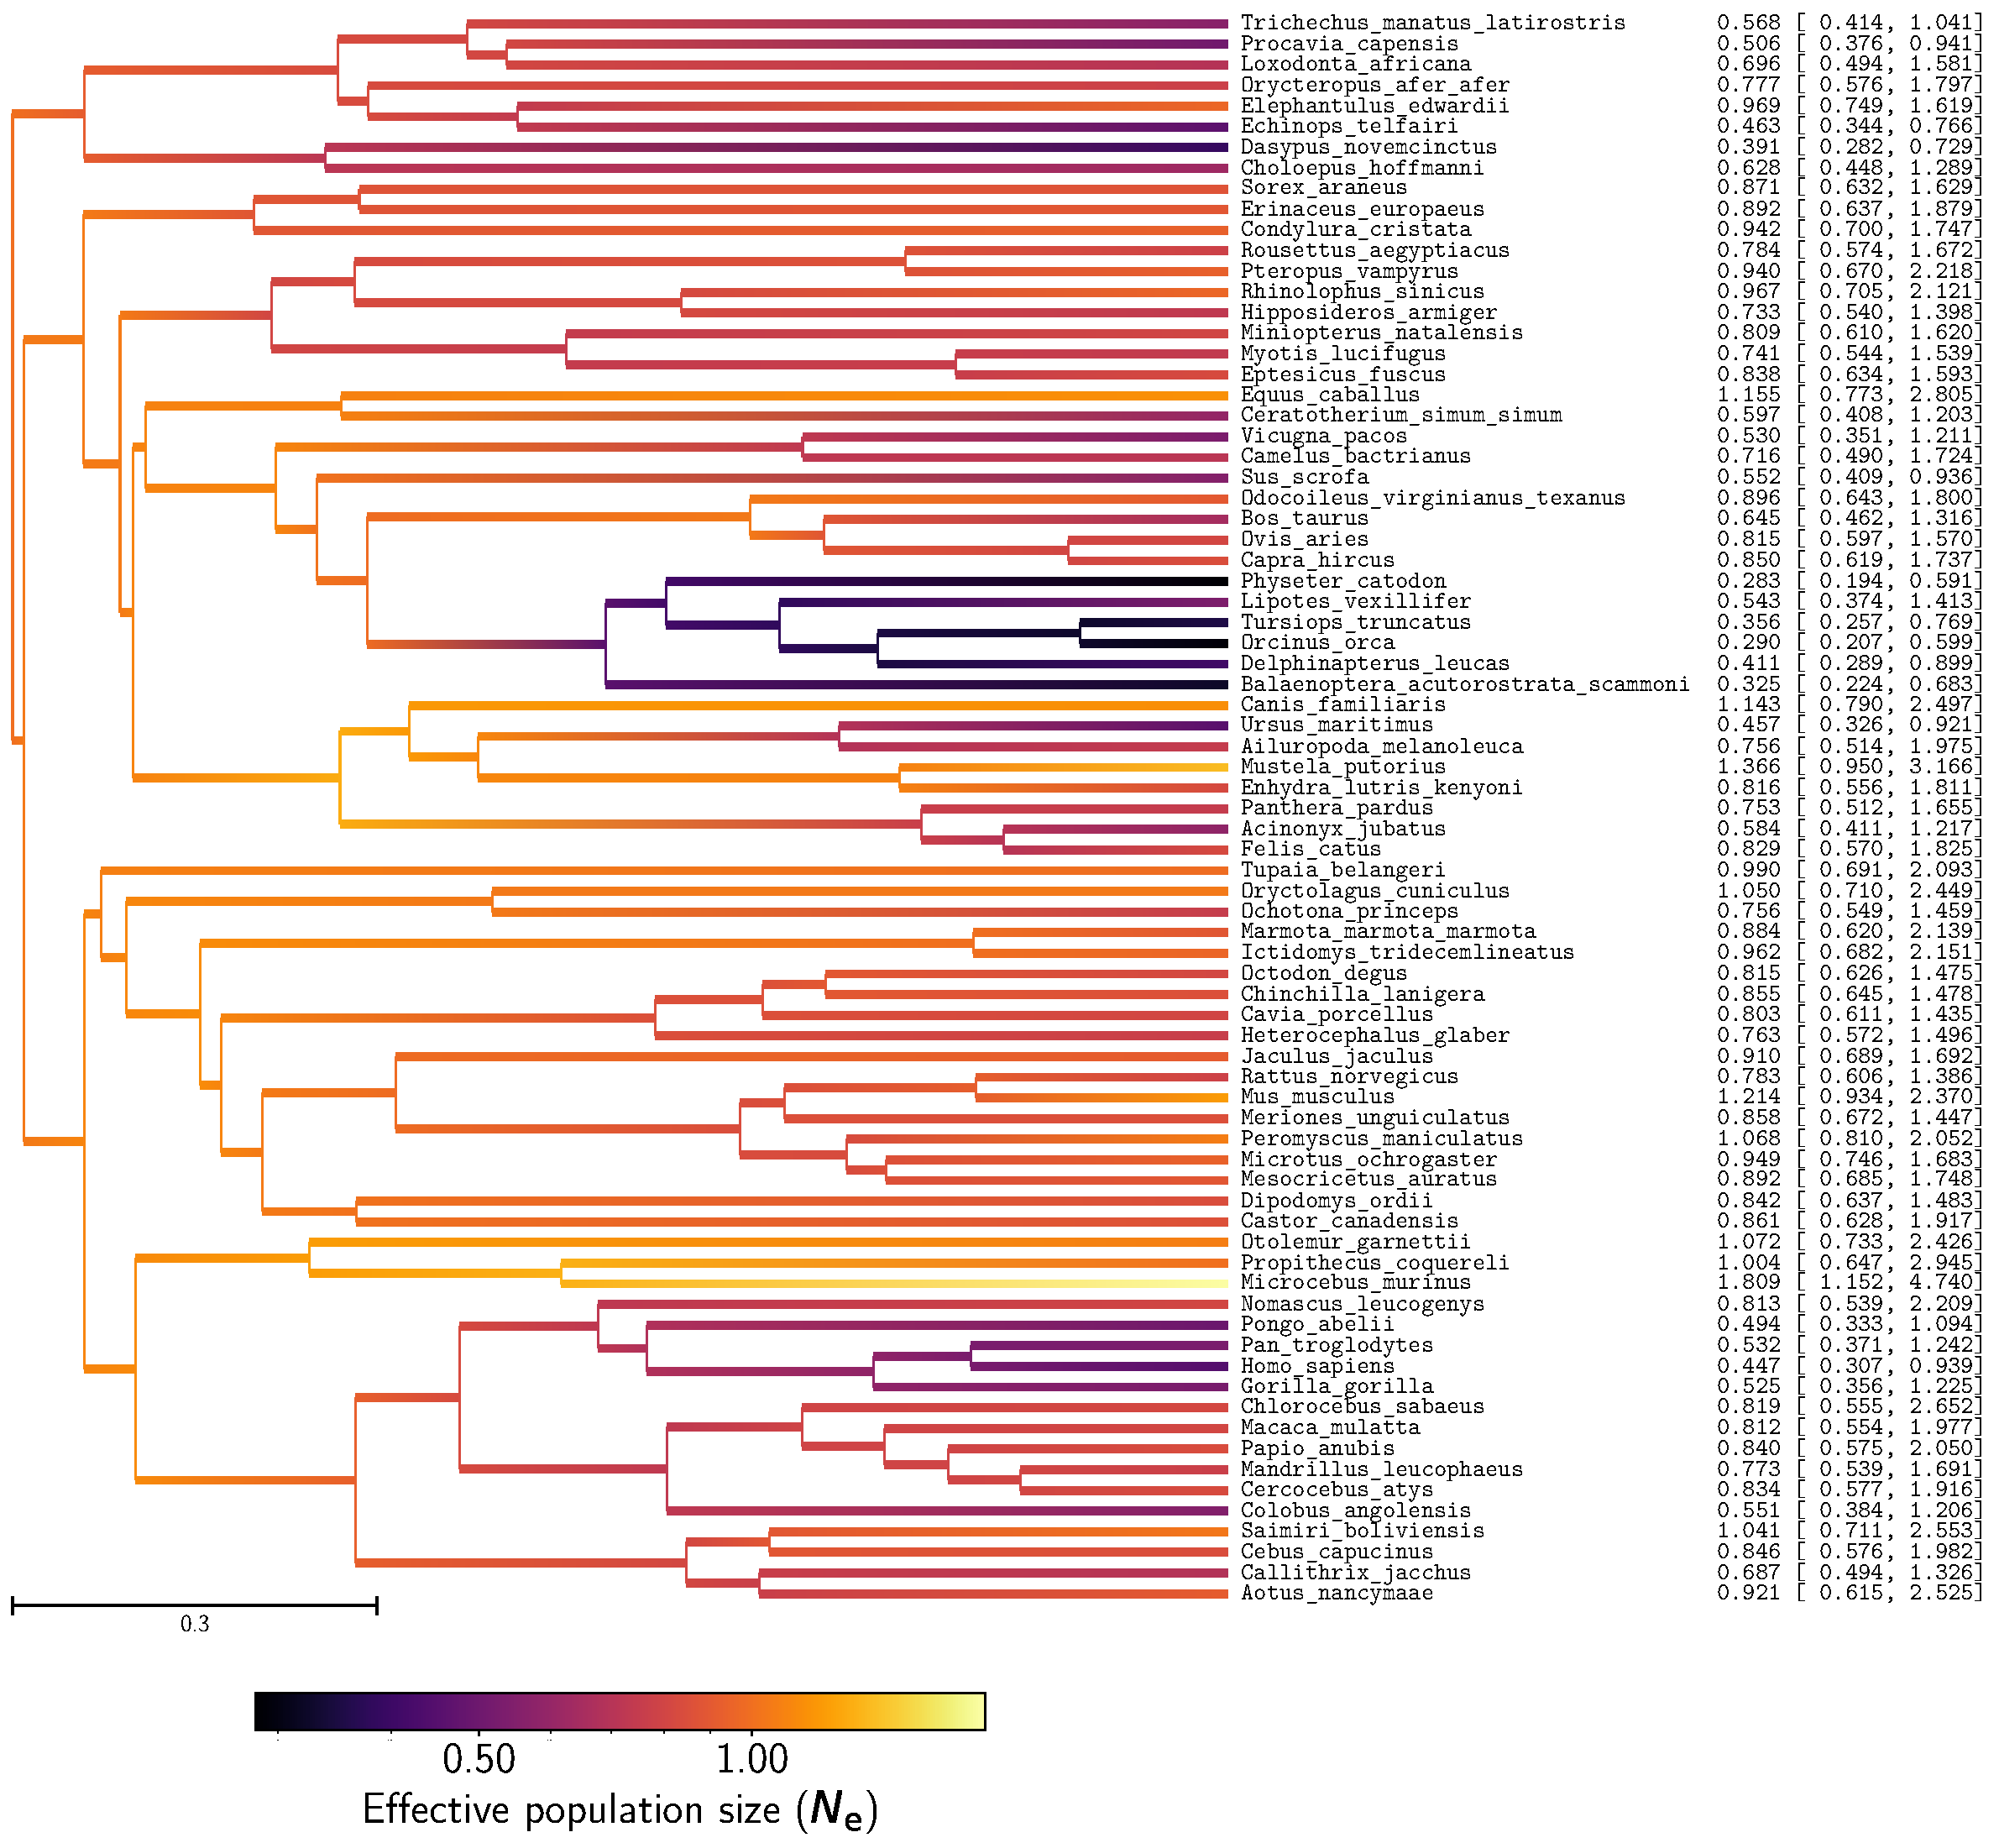
\includegraphics[width=\linewidth, page=1]{mammals/18CDS_SiteMutSelBranchNe_R1_LogPopulationSize}
		\caption[$\Ne$ estimation in mammals]{Effective population size ($\Ne$) estimation in mammals}
	\end{figure}

	\begin{figure}[H]
		\centering
		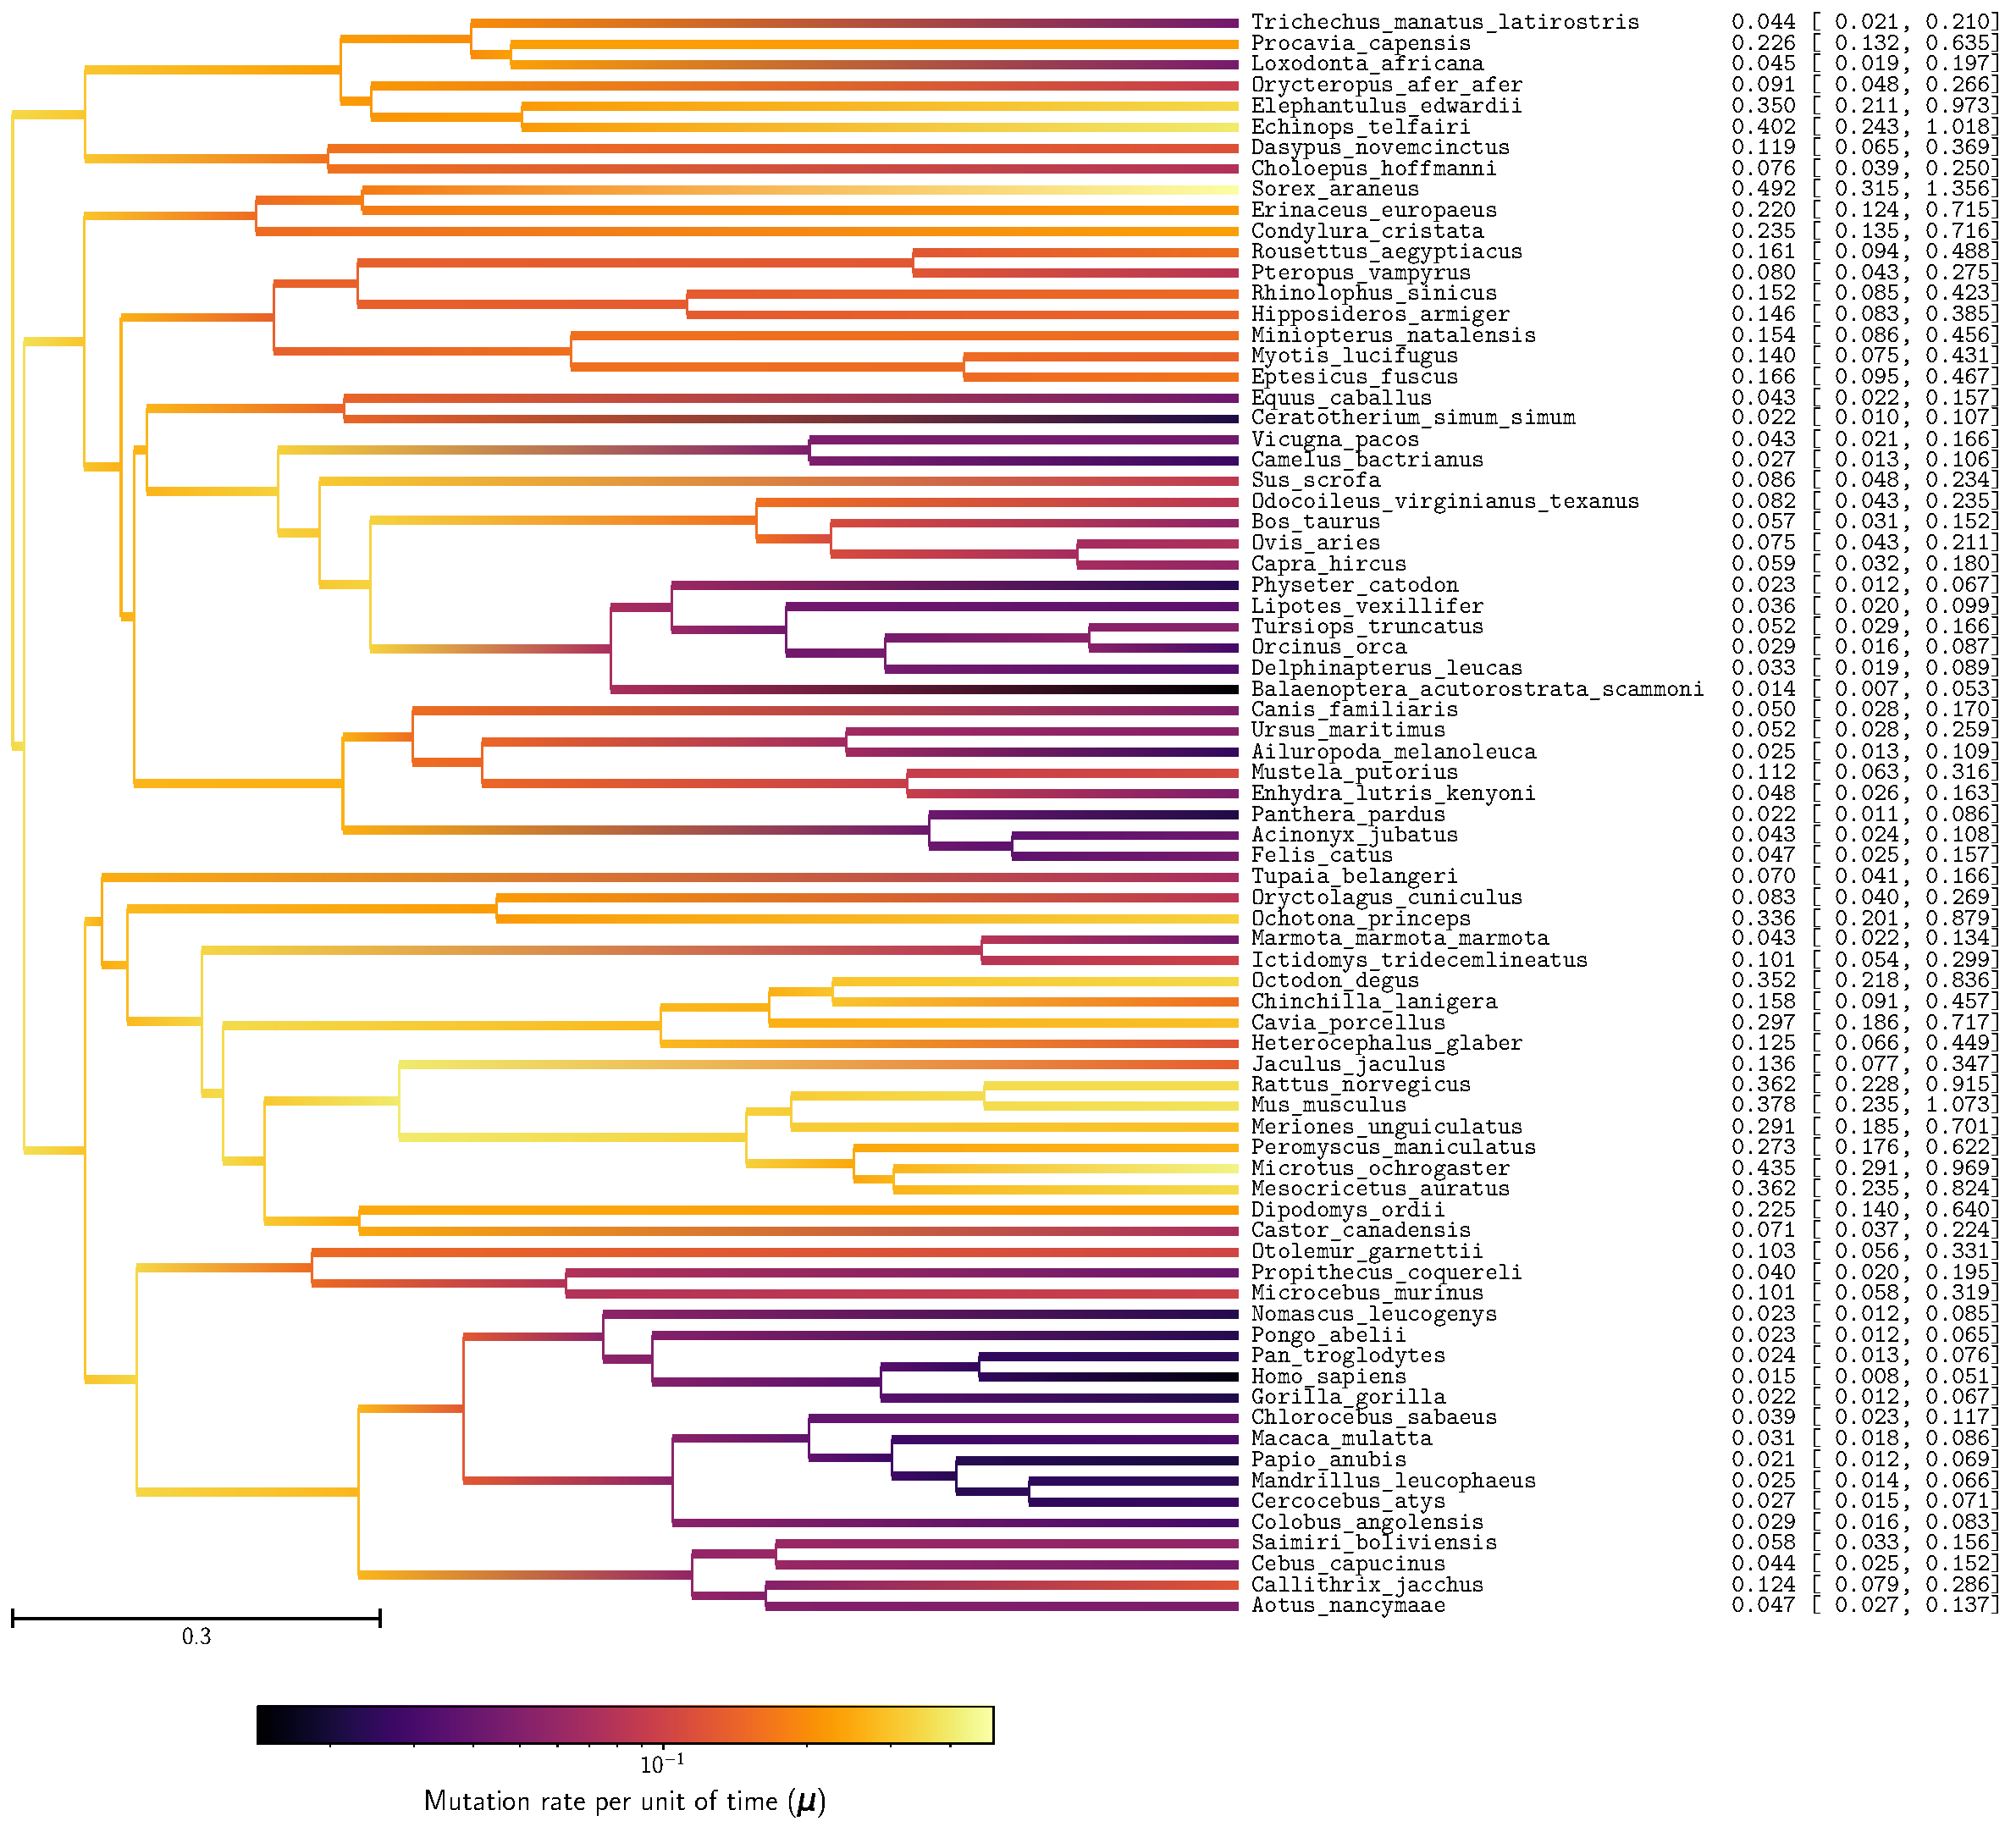
\includegraphics[width=\linewidth, page=1]{mammals/18CDS_SiteMutSelBranchNe_R1_LogMutationRatePerTime}
		\caption[Mutation rate estimation in mammals]{Mutation rate ($\mu$) estimation in mammals}
	\end{figure}

	\begin{figure}[H]
		\centering
		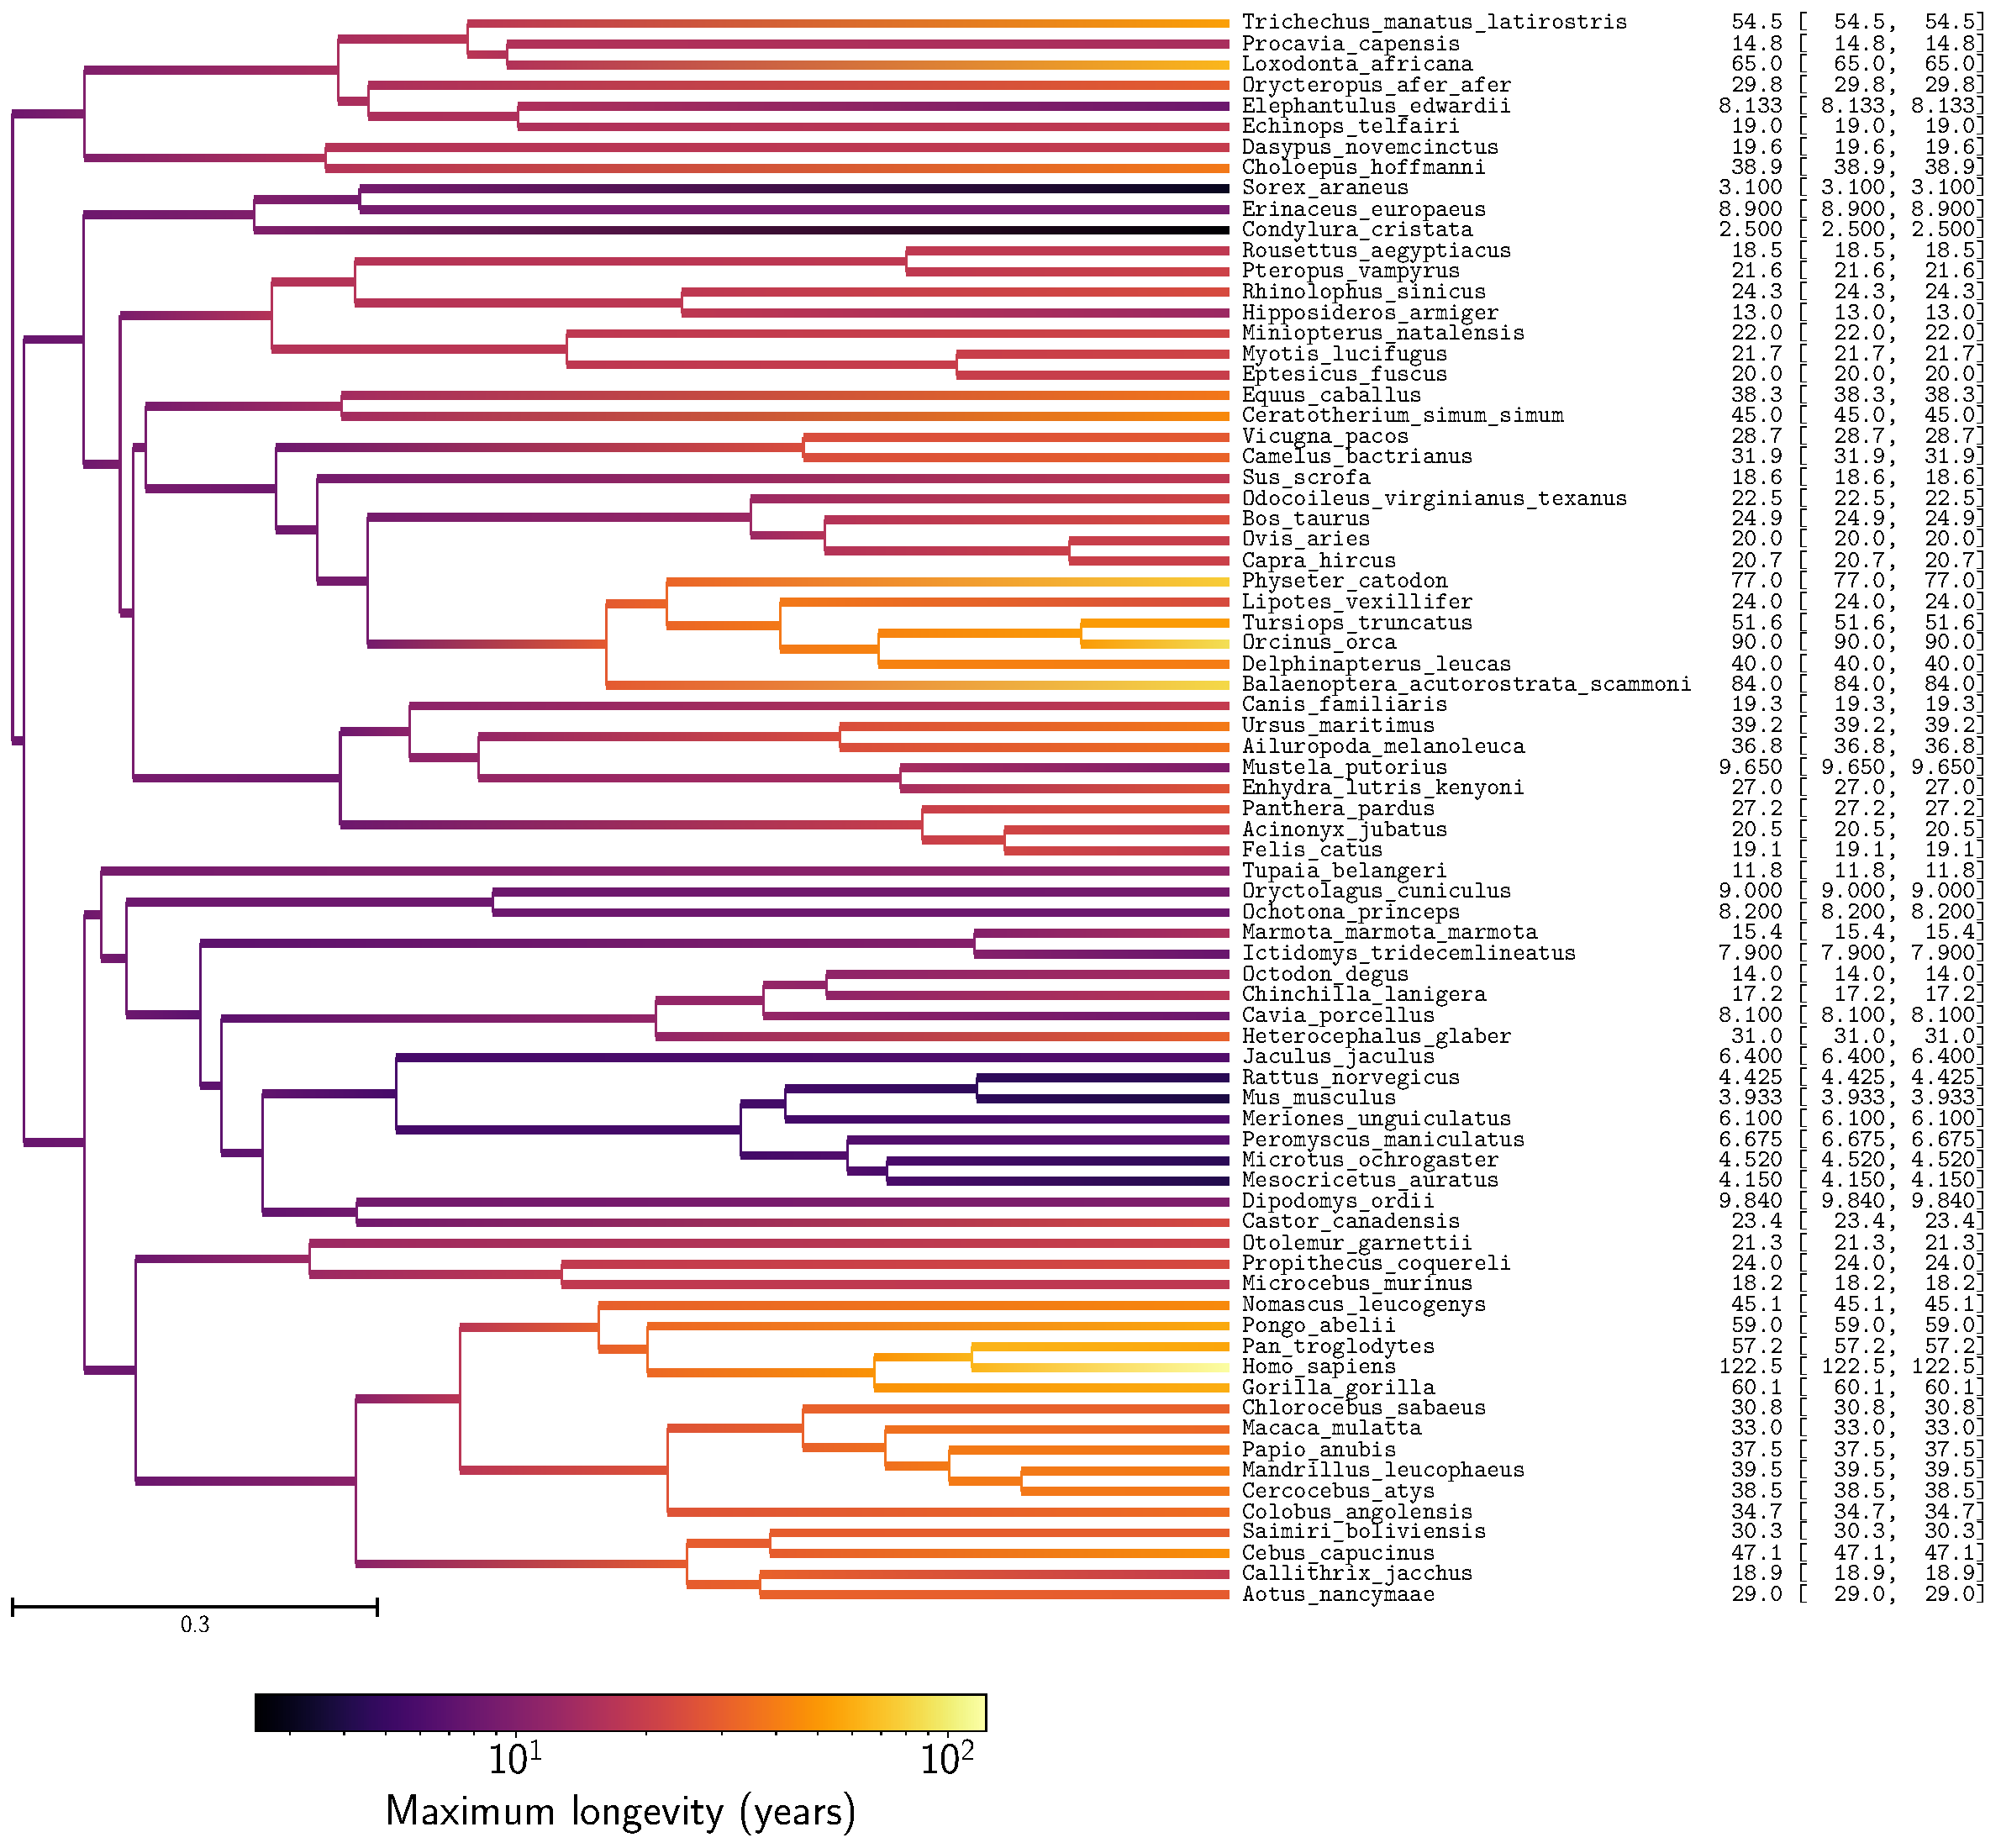
\includegraphics[width=\linewidth, page=1]{mammals/18CDS_SiteMutSelBranchNe_R1_LogMaximum_longevity}
		\caption[Maximum longevity estimation in mammals]{Maximum longevity estimation in mammals}
	\end{figure}

	\begin{figure}[H]
		\centering
		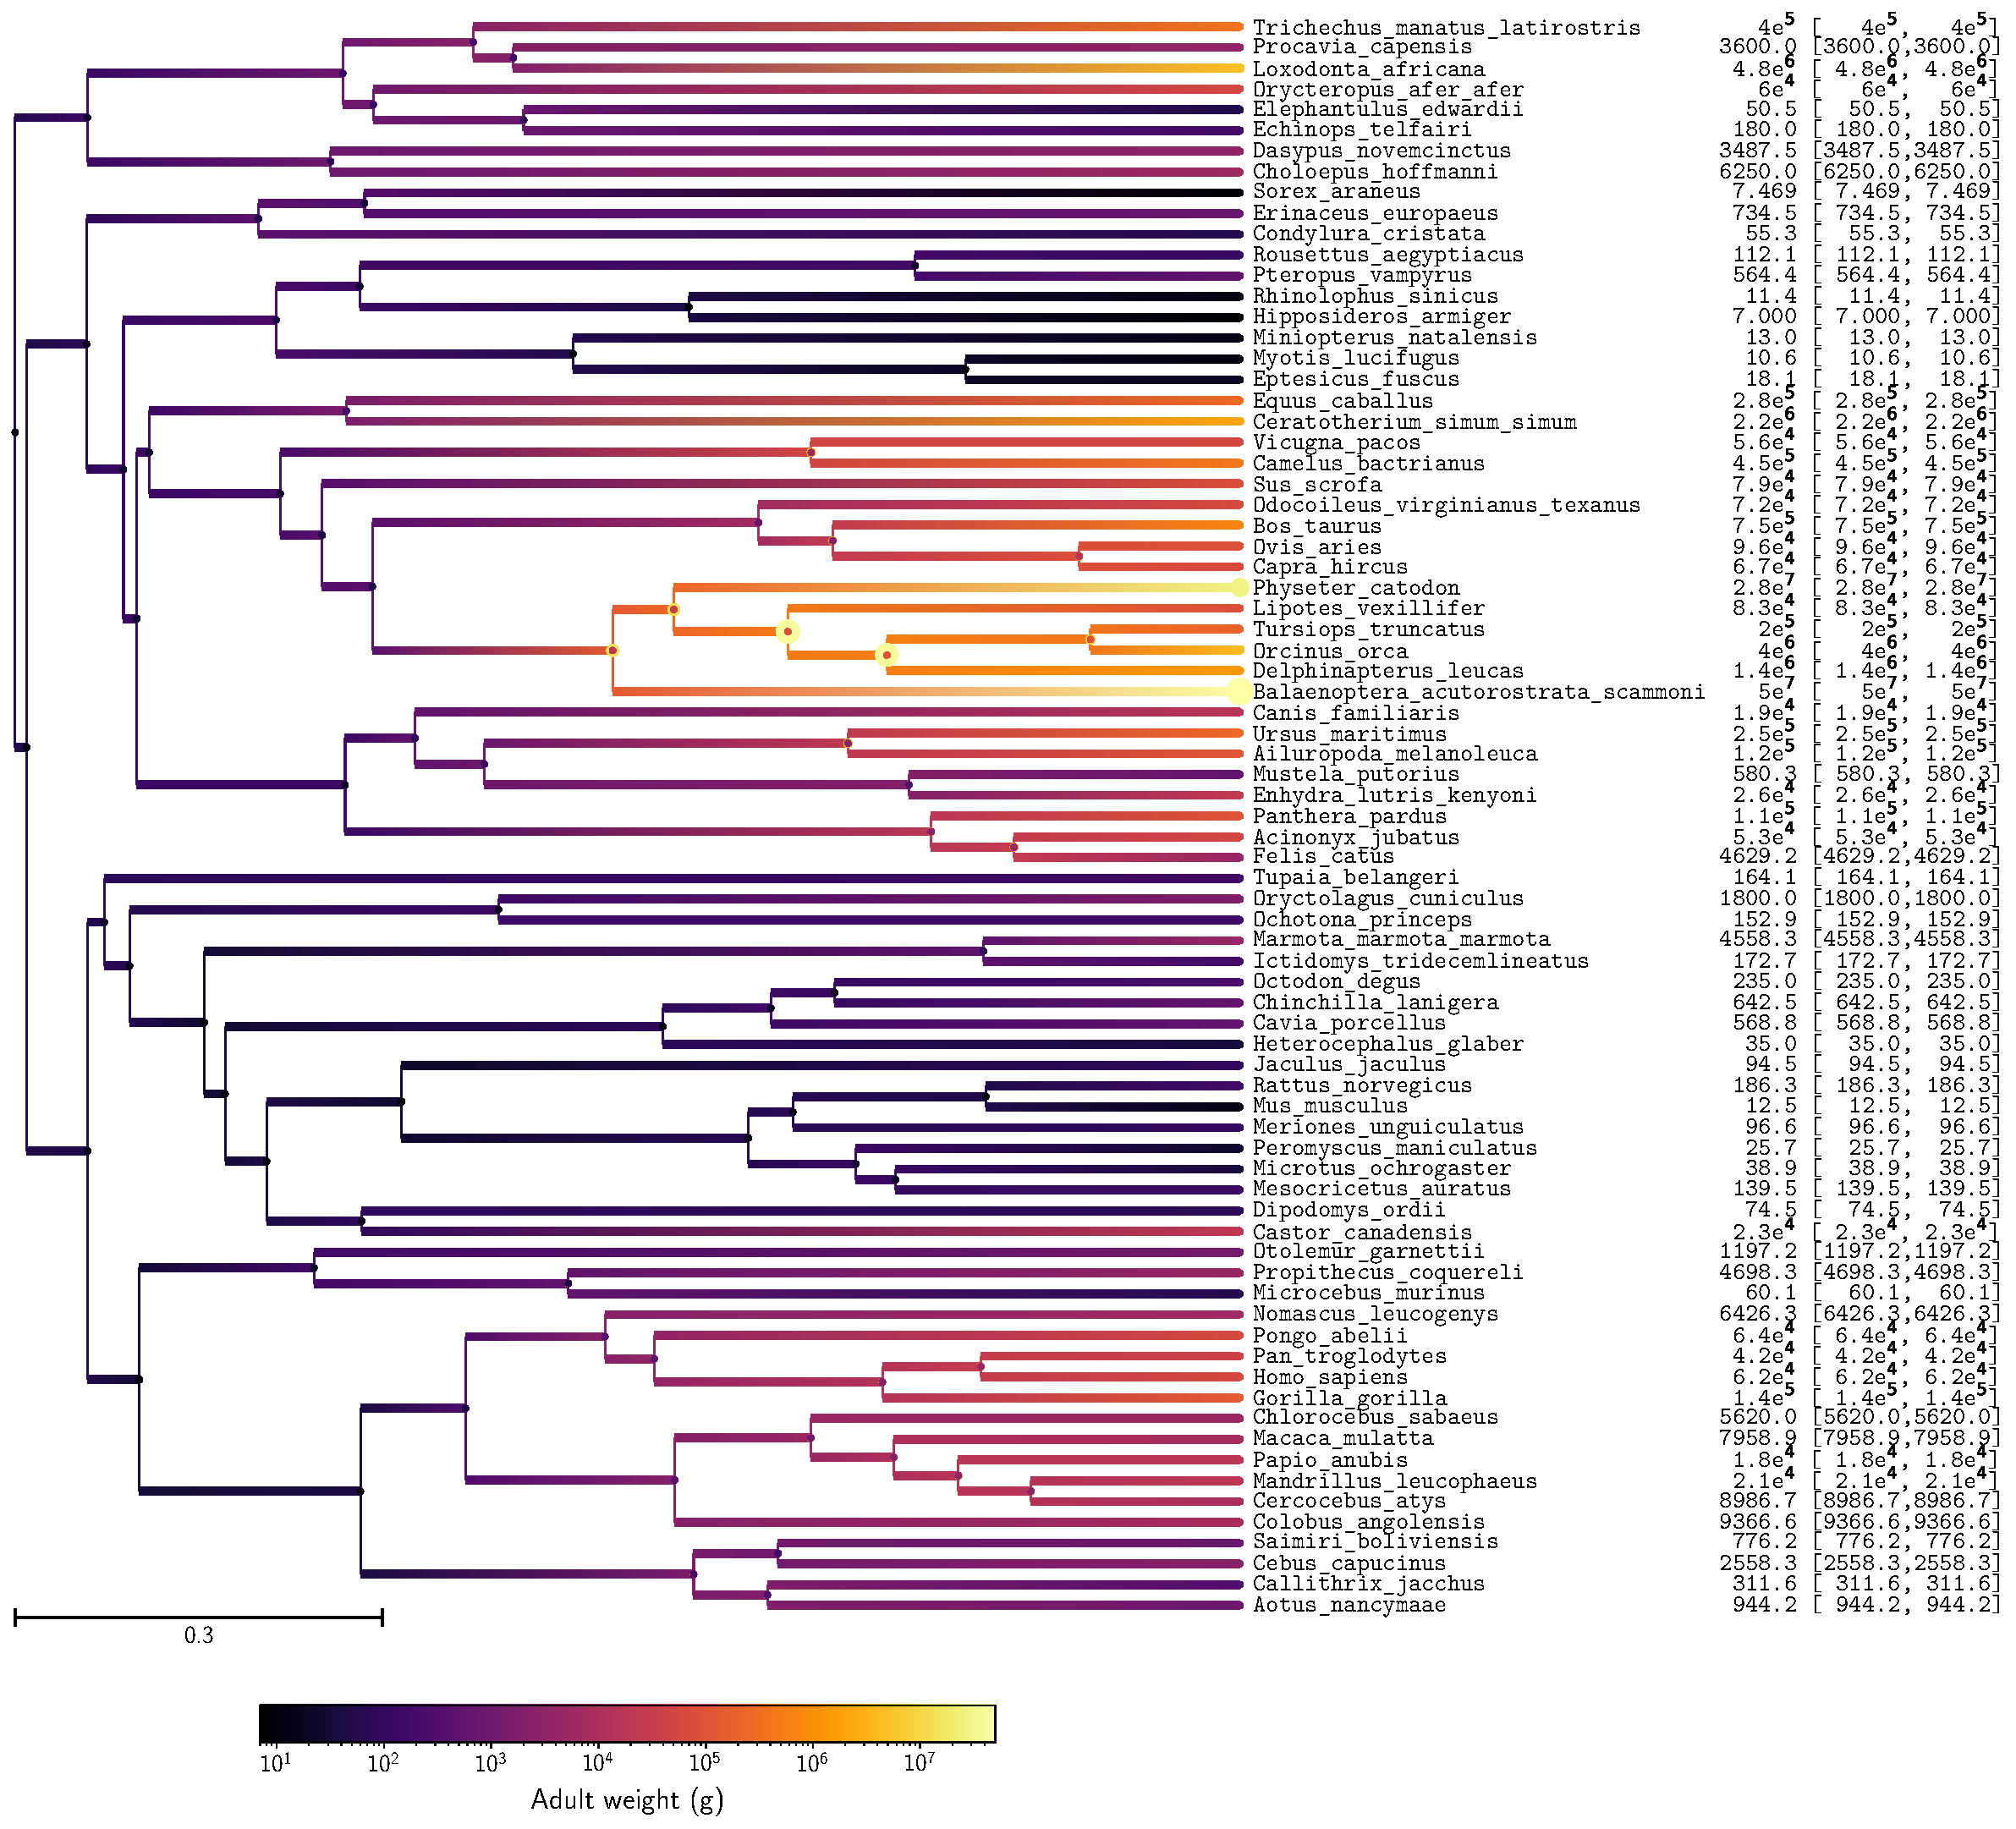
\includegraphics[width=\linewidth, page=1]{mammals/18CDS_SiteMutSelBranchNe_R1_LogAdult_weight}
		\caption[Adult weight estimation in mammals]{Adult weight estimation in mammals}
	\end{figure}

	\begin{figure}[H]
		\centering
		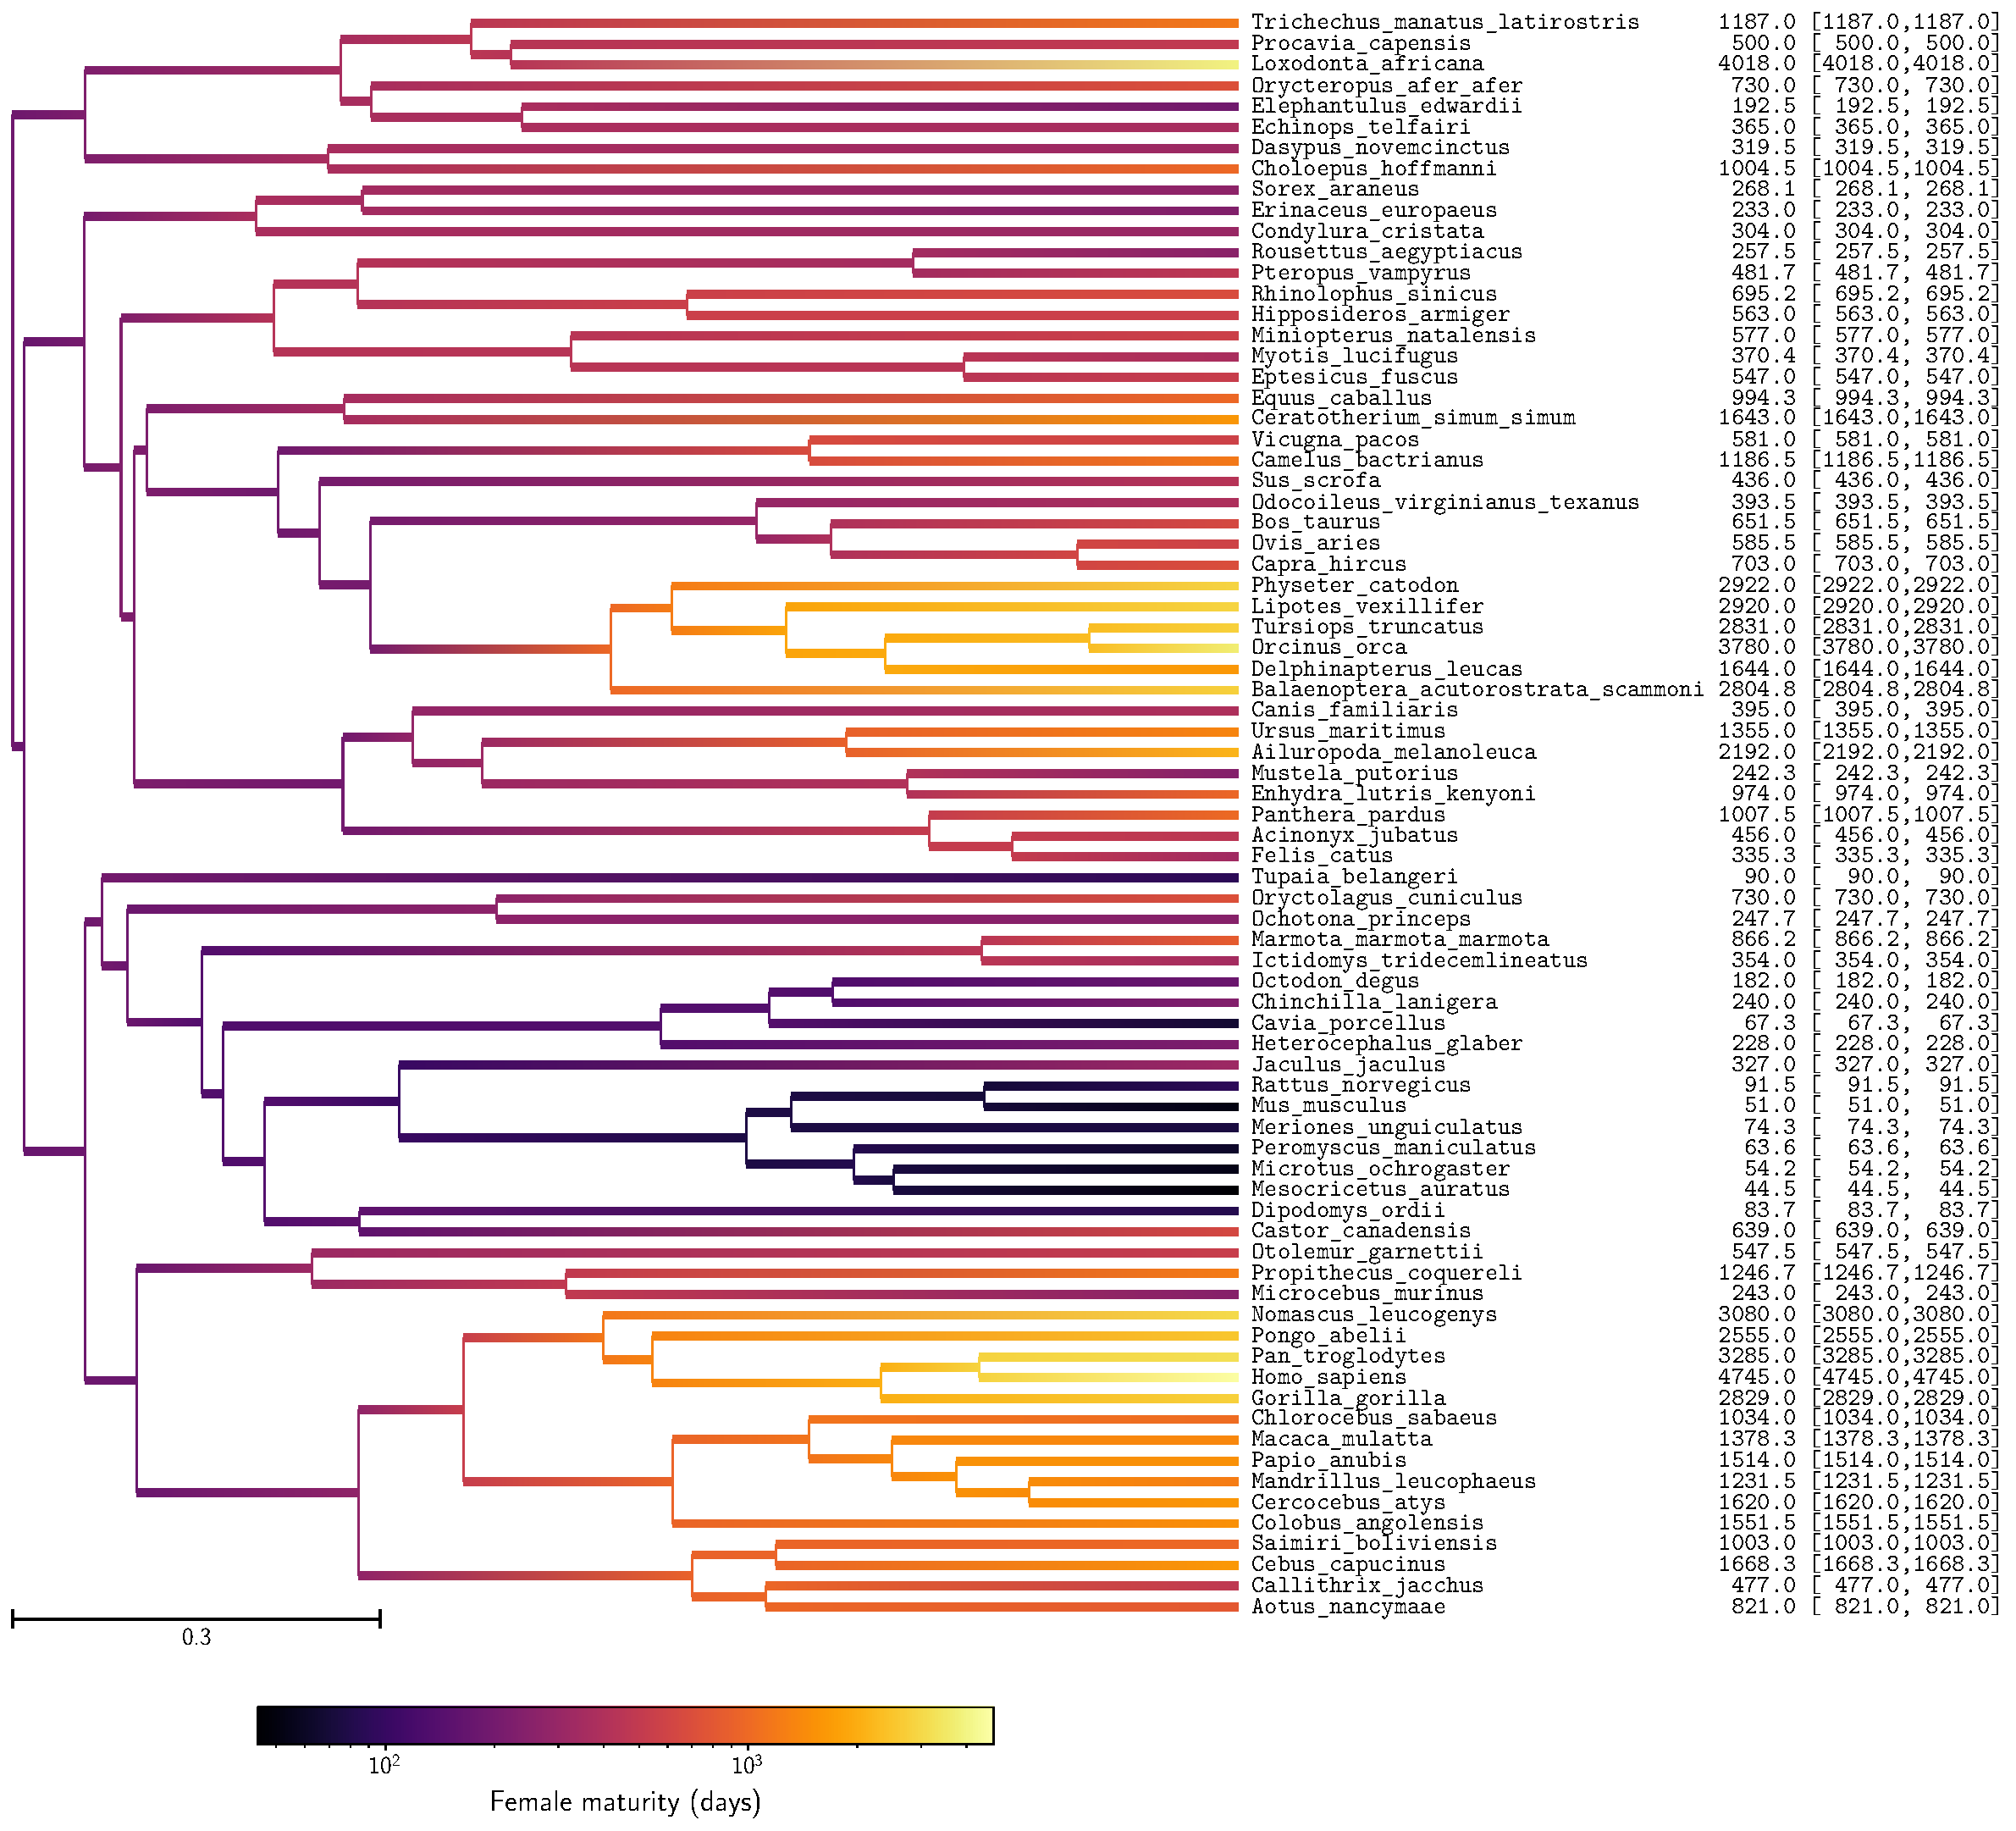
\includegraphics[width=\linewidth, page=1]{mammals/18CDS_SiteMutSelBranchNe_R1_LogFemale_maturity}
		\caption[Female maturity estimation in mammals]{Female maturity estimation in mammals}
	\end{figure}

	\subsection{Repeatability of experiments}
	\label{subsec:repeatability-of-experiments-mammals}

	$4$ independent inferences were performed on a randomly chosen set of $18$ coding sequences ({CDS}) out of $226$.
	Obtained with the mechanistic inference model developed in this paper of site-specific amino-acid fitness profiles and log-Brownian process for $\Ne$, $\mu$ and life-history traits.
	Each plot is a correlation between a pair of experiments for a given parameter.
	For each node (or branch) of the tree, the mean {posterior} of the parameter over the {MCMC} (after burn-in) is represented in blue dots, green solid lines are the $90\%$ confidence interval of the {MCMC}.
	Solid red line is the regression line between replicates.

	\begin{figure}[H]
		\centering
		\begin{minipage}{0.32\linewidth}
			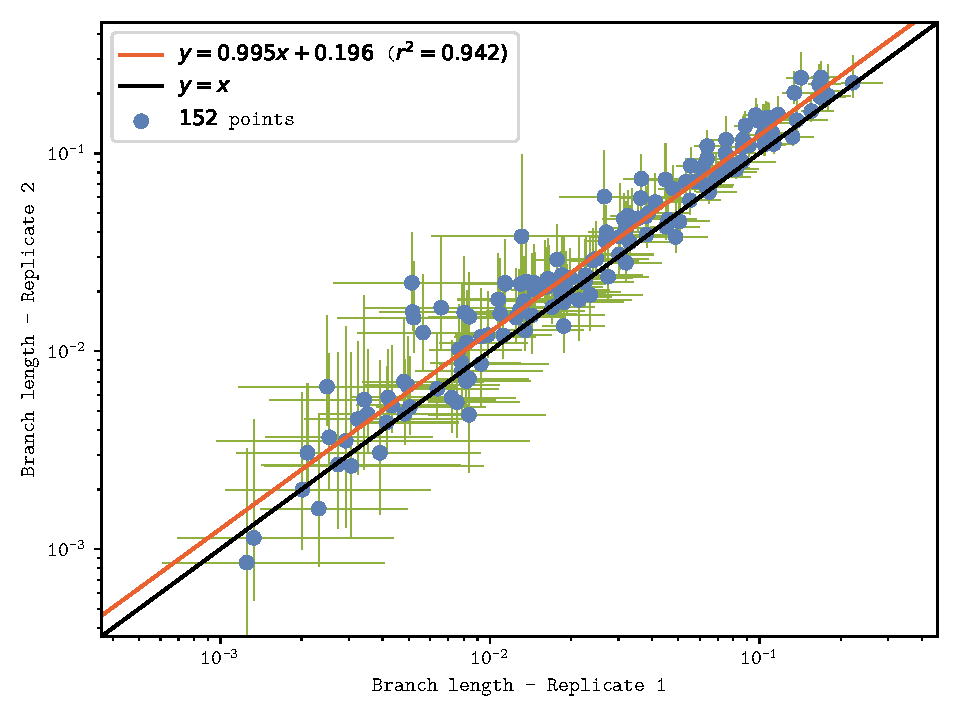
\includegraphics[width=\linewidth, page=1]{mammals/18CDS_SiteMutSelBranchNe_Rep_Log10BranchLength-1-2}
		\end{minipage} \hfill
		\begin{minipage}{0.32\linewidth}
			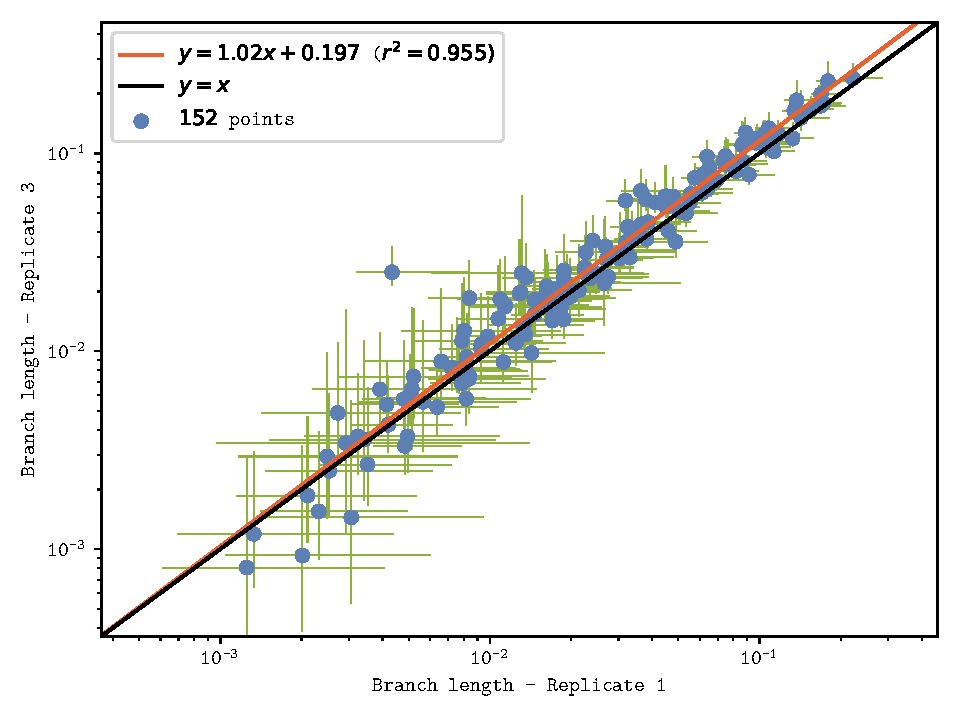
\includegraphics[width=\linewidth, page=1]{mammals/18CDS_SiteMutSelBranchNe_Rep_Log10BranchLength-1-3}
		\end{minipage} \hfill
		\begin{minipage}{0.32\linewidth}
			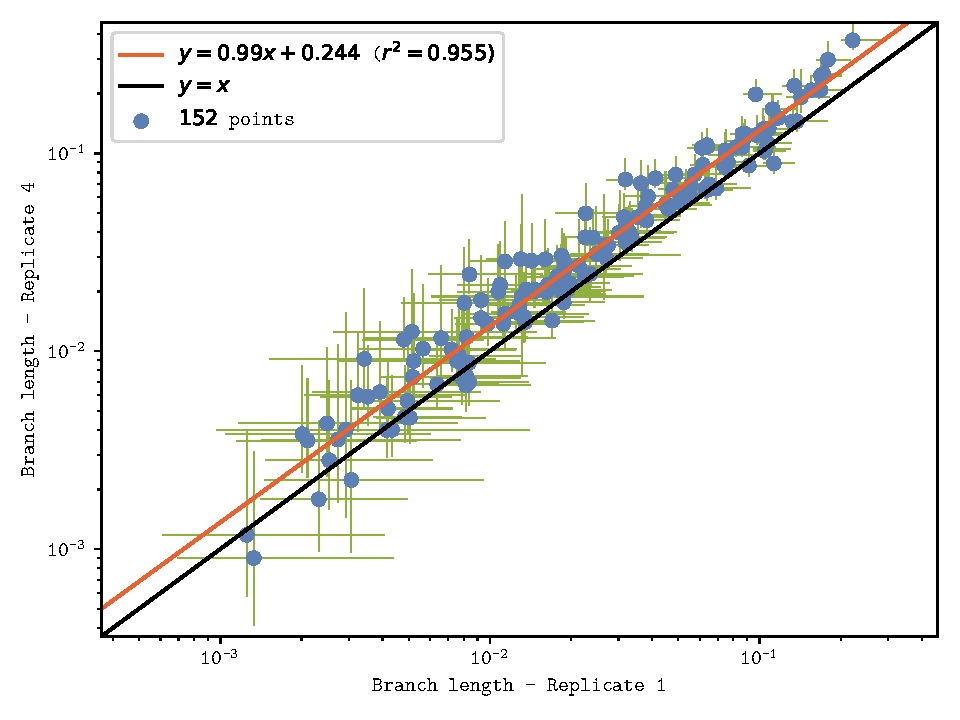
\includegraphics[width=\linewidth, page=1]{mammals/18CDS_SiteMutSelBranchNe_Rep_Log10BranchLength-1-4}
		\end{minipage}
		\caption[Repeatability of branch length estimation in mammals]{Repeatability of branch length ($\branchlength$) estimation in mammals}
	\end{figure}

	\begin{figure}[H]
		\centering
		\begin{minipage}{0.32\linewidth}
			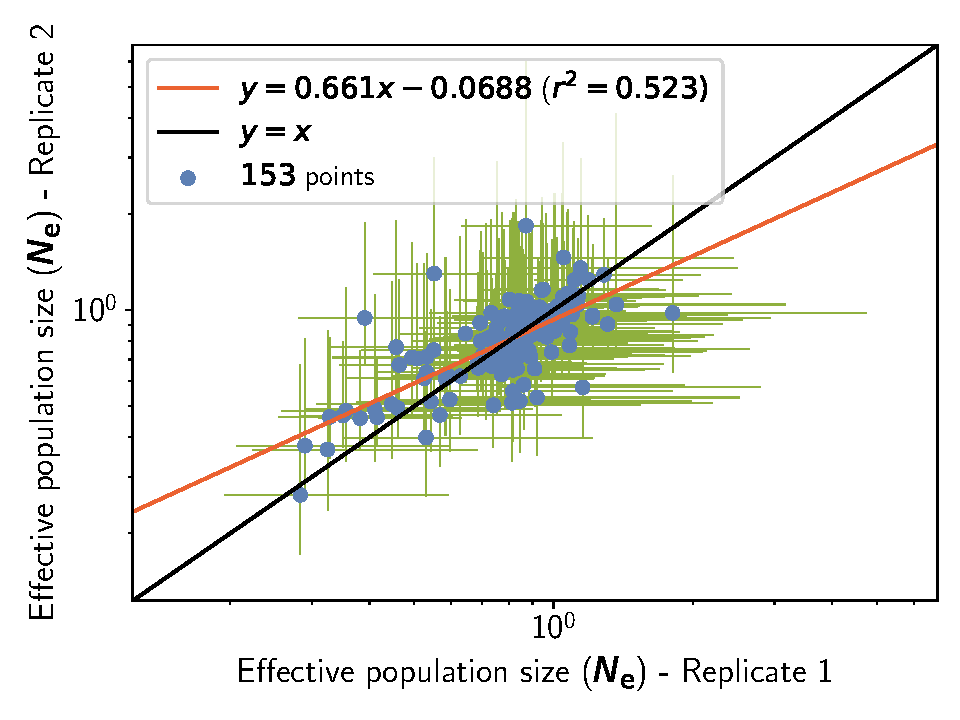
\includegraphics[width=\linewidth, page=1]{mammals/18CDS_SiteMutSelBranchNe_Rep_LogPopulationSize-1-2}
		\end{minipage} \hfill
		\begin{minipage}{0.32\linewidth}
			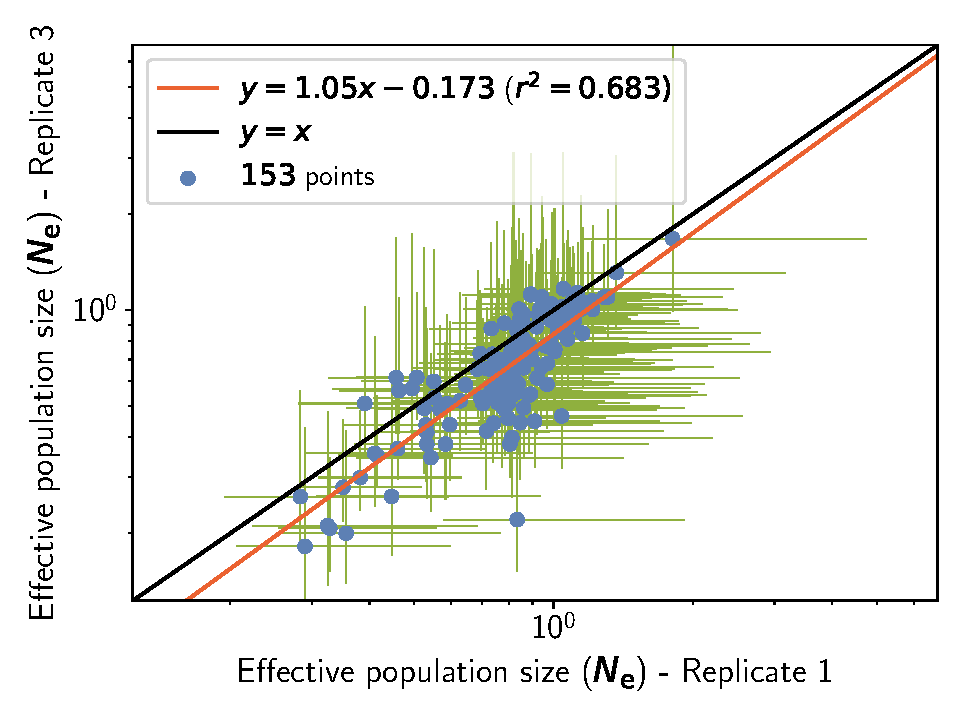
\includegraphics[width=\linewidth, page=1]{mammals/18CDS_SiteMutSelBranchNe_Rep_LogPopulationSize-1-3}
		\end{minipage} \hfill
		\begin{minipage}{0.32\linewidth}
			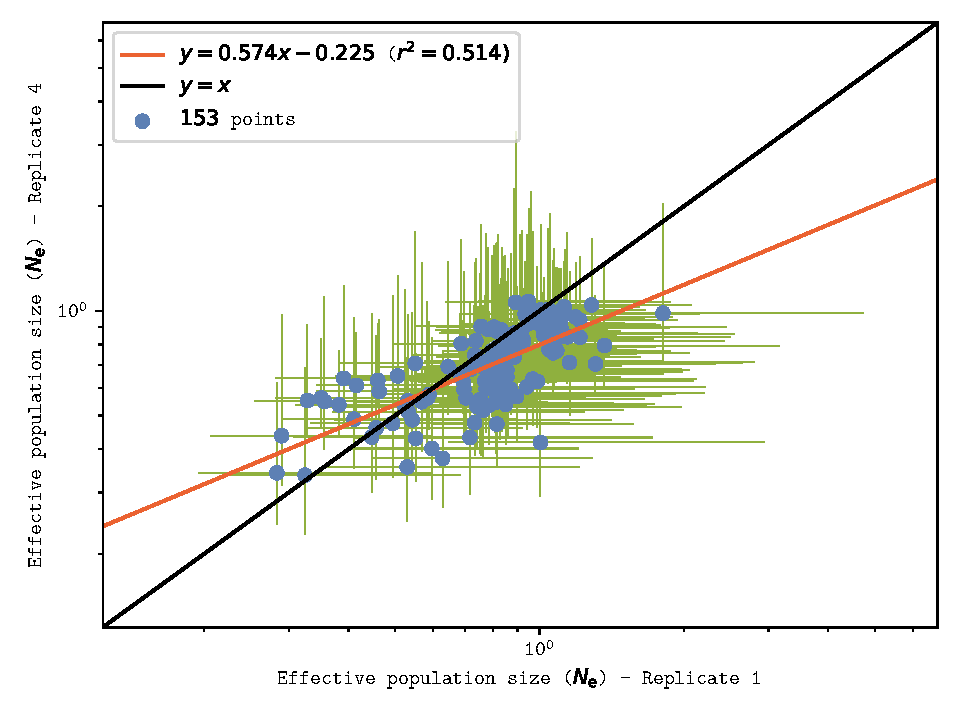
\includegraphics[width=\linewidth, page=1]{mammals/18CDS_SiteMutSelBranchNe_Rep_LogPopulationSize-1-4}
		\end{minipage}
		\caption[Repeatability of $\Ne$ estimation in mammals]{Repeatability of {effective population size} ($\Ne$) estimation in mammals}
	\end{figure}

	\begin{table}[htbp]
		\renewcommand{\arraystretch}{0.5}
		\scriptsize \centering
		\begin{tabular}{lllll}
\toprule
         Rep. 1 &          Rep. 2 &          Rep. 3 &          Rep. 4 &                   Taxon \\
\midrule
           1.24 &             8.1 &           0.877 &            2.03 &           Slebanonensis \\
           2.02 &            1.54 &           0.821 &             1.5 &               Darizonae \\
           1.32 &            2.12 &            1.94 &            1.81 &                    dmoj \\
           1.22 &            2.48 &           0.271 &            1.39 &                Dnavojoa \\
          0.987 &               2 &           0.762 &            1.15 &            me07rcatorum \\
            1.4 &            2.22 &            1.11 &            1.54 &            me39rcatorum \\
           2.05 &            8.48 &            1.63 &            2.88 &                  Dhydei \\
           1.55 &            2.57 &           0.651 &            1.06 &              Damericana \\
           1.88 &            2.94 &           0.986 &            1.07 &           Dnovamexicana \\
            1.5 &             2.9 &           0.896 &            1.97 &                    dvir \\
          0.344 &           0.912 &            0.52 &           0.929 &                Dmontana \\
           1.83 &            2.36 &            1.02 &           0.961 &                Drobusta \\
           1.99 &            4.19 &           0.875 &            2.71 &               Dmelanica \\
           1.92 &            2.58 &            1.03 &            1.25 &          Dmicromelanica \\
           1.73 &            4.08 &            1.26 &            1.36 &              Dlacertosa \\
            1.3 &            4.38 &            1.22 &            2.55 &                    dgri \\
           0.97 &           0.765 &           0.554 &           0.614 &              Zafricanus \\
           1.04 &            1.41 &           0.408 &           0.482 &              Zgabonicus \\
            1.4 &             3.4 &            1.52 &            1.82 &               Zindianus \\
           2.61 &           0.297 &            1.35 &            1.38 &             Dalbomicans \\
           1.28 &            3.35 &            0.66 &            2.85 &                 Dnasuta \\
            1.5 &            4.13 &            1.44 &            1.95 &                Dbusckii \\
            2.3 &            3.75 &            1.46 &            2.12 &                psaltans \\
           2.36 &           0.789 &            1.77 &            2.37 &                nebulosa \\
           1.73 &            3.58 &            1.55 &            2.17 &                    dwil \\
          0.697 &           0.864 &           0.743 &           0.515 &              paulistrom \\
           1.55 &            2.74 &            1.31 &            2.29 &            equinoxialis \\
           2.19 &            3.66 &            1.37 &            1.08 &                  azteca \\
           1.23 &            2.47 &            1.22 &               2 &               athabasca \\
          0.626 &            1.95 &           0.814 &           0.428 &              Dathabasca \\
           1.42 &            1.53 &            1.65 &            1.17 &                 affinis \\
           1.25 &            2.11 &            1.54 &           0.873 &                    Dpse \\
          0.944 &            1.78 &           0.469 &           0.241 &                    dper \\
          0.891 &            3.79 &           0.495 &           0.981 &                Dmiranda \\
           1.12 &            2.94 &            1.19 &            2.03 &                 obscura \\
           1.01 &            5.79 &            1.16 &           0.985 &                Dobscura \\
           1.38 &            1.98 &             1.4 &            1.66 &                 ambigua \\
           1.64 &            3.62 &            1.74 &            1.89 &                   imaii \\
           2.11 &            2.85 &            1.23 &            1.63 &              bifasciata \\
           1.47 &            2.22 &            1.21 &            1.42 &            tsukubaensis \\
           1.45 &            2.76 &           0.911 &            1.09 &                 guanche \\
           1.37 &            3.33 &            1.22 &           0.944 &                Dguanche \\
            1.5 &            1.78 &            1.29 &            1.98 &              subobscura \\
           1.92 &            2.23 &            1.46 &            2.05 &             Dsubobscura \\
          0.978 &            2.95 &           0.907 &            1.58 &              microlabis \\
           1.34 &            3.16 &            1.64 &            1.64 &             Dmauritiana \\
           1.02 &            2.31 &           0.777 &            1.28 &                    dsim \\
           1.32 &            2.05 &            0.95 &            1.16 &                    dsec \\
           1.89 &            2.59 &            1.48 &            1.62 &                   BDGP6 \\
           1.63 &            2.77 &            1.32 &            1.65 &               teissieri \\
           1.96 &            3.62 &            1.14 &            2.19 &                    dyak \\
           1.22 &            2.66 &           0.837 &            1.48 &                    dere \\
           1.71 &            4.37 &            1.21 &            1.93 &             Deugracilis \\
            2.1 &            2.78 &            1.46 &            2.06 &               lutescens \\
          0.889 &           0.756 &               1 &           0.966 &               paralutea \\
           1.83 &            1.86 &               2 &            1.78 &             Dtakahashii \\
           2.32 &            2.11 &           0.901 &            2.52 &            prostipennis \\
            1.8 &            3.42 &            1.78 &            2.22 &             pstakahashi \\
           1.92 &            3.83 &           0.824 &            2.33 &                mimetica \\
            1.6 &            5.09 &            1.07 &               2 &                Dsuzukii \\
           2.27 &            2.85 &            1.24 &            1.62 &              Dbiarmipes \\
           1.95 &            4.12 &             1.6 &            1.39 &                Delegans \\
           1.16 &            2.89 &            1.26 &            1.47 &              lucipennis \\
            3.1 &            5.48 &            1.74 &            4.27 &             Dficusphila \\
           1.53 &            2.66 &           0.456 &            1.99 &             diplacantha \\
           1.52 &            2.76 &            1.58 &            1.31 &                 ercepae \\
           1.52 &            2.35 &            1.29 &            2.67 &                barbarae \\
           1.91 &            2.71 &            1.72 &            1.68 &                Dserrata \\
           2.25 &            5.33 &            1.59 &            2.66 &               Dkikkawai \\
           1.37 &            2.64 &            1.14 &            1.46 &             phaeopleura \\
            1.8 &            2.72 &            1.24 &            1.33 &                    dana \\
           1.71 &            3.87 &             1.5 &            2.57 &               pallidosa \\
           1.71 &            2.77 &            1.43 &            1.92 &           malerkotliana \\
           1.59 &            2.72 &            1.49 &            1.85 &            Dbipectinata \\
           1.03 &            2.07 &            1.38 &            1.64 &            pbipectinata \\
          0.999 &            0.95 &           0.525 &           0.821 &         pseudoananassae \\
           2.48 &            5.18 &             1.2 &            2.73 &                 varians \\
 \textbf{ 9.02} &  \textbf{ 28.5} &  \textbf{ 7.36} &  \textbf{ 17.7} &  \textbf{Maximum range} \\
\bottomrule
\end{tabular}

		\caption[Repeatability of $\Ne$ estimation in mammals]{Repeatability of {effective population size} ($\Ne$) estimation in mammals, for the extant taxa.}
		\label{tab:Ne-estimated-mammals}
	\end{table}

	\begin{figure}[H]
		\centering
		\begin{minipage}{0.32\linewidth}
			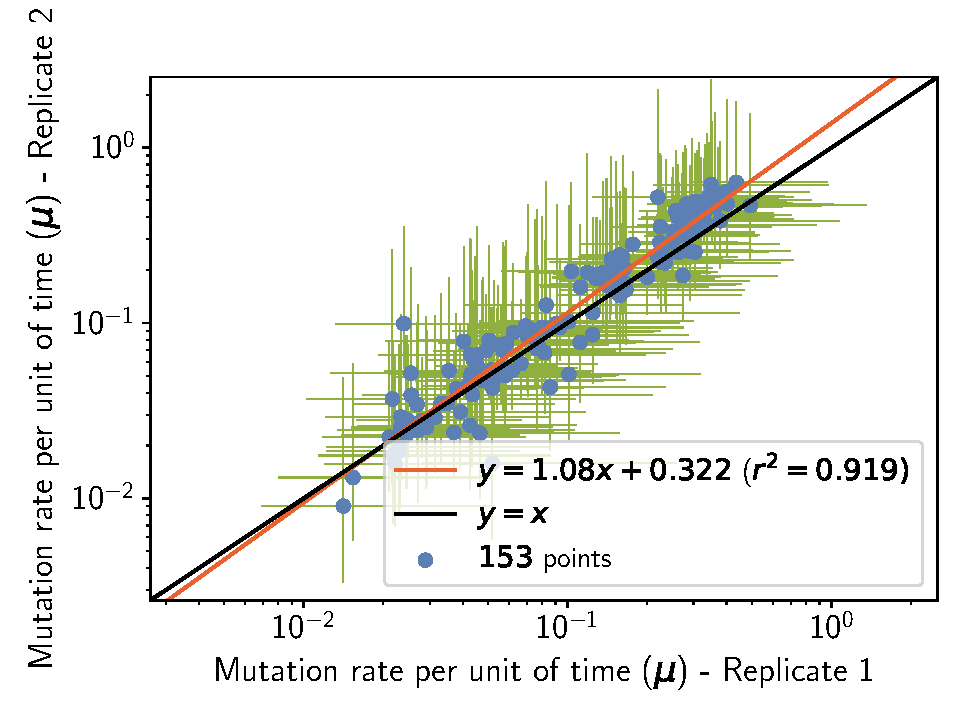
\includegraphics[width=\linewidth, page=1]{mammals/18CDS_SiteMutSelBranchNe_Rep_LogMutationRatePerTime-1-2}
		\end{minipage} \hfill
		\begin{minipage}{0.32\linewidth}
			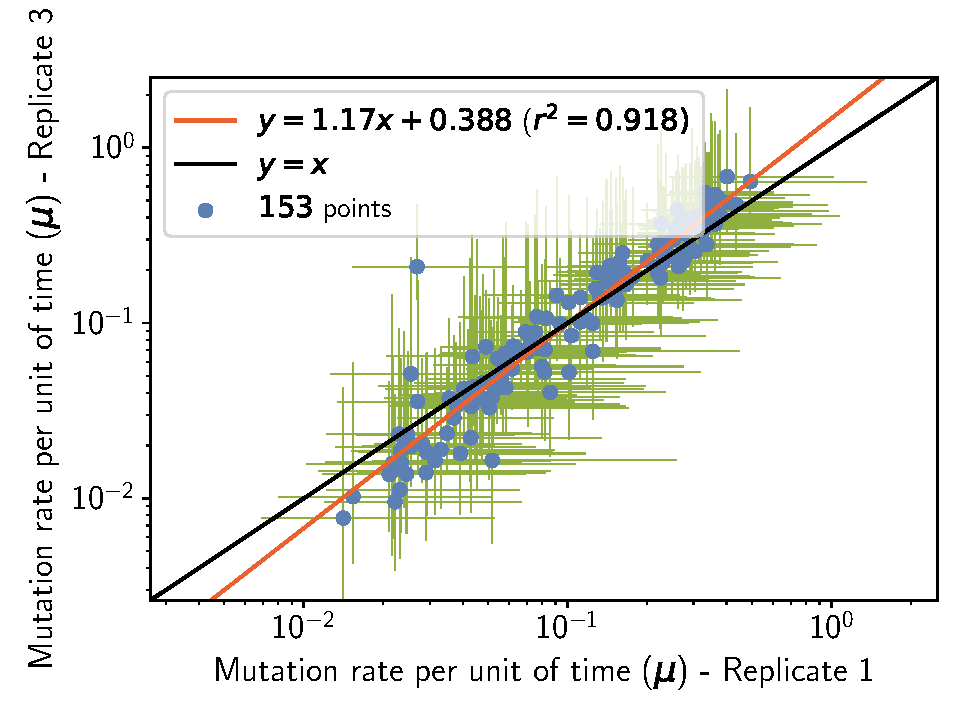
\includegraphics[width=\linewidth, page=1]{mammals/18CDS_SiteMutSelBranchNe_Rep_LogMutationRatePerTime-1-3}
		\end{minipage} \hfill
		\begin{minipage}{0.32\linewidth}
			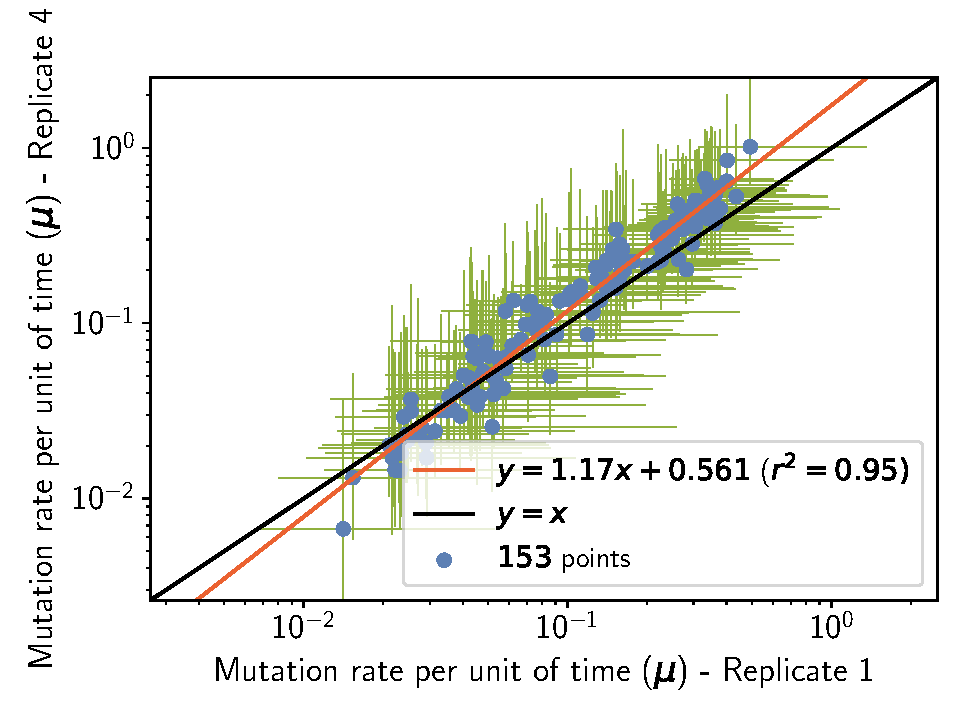
\includegraphics[width=\linewidth, page=1]{mammals/18CDS_SiteMutSelBranchNe_Rep_LogMutationRatePerTime-1-4}
		\end{minipage}
		\caption[Repeatability of mutation rate estimation in mammals]{Repeatability of mutation rate ($\mu$) estimation in mammals}
	\end{figure}

	\begin{table}[htbp]
		\renewcommand{\arraystretch}{0.5}
		\scriptsize \centering
		\begin{tabular}{lllll}
\toprule
         Rep. 1 &          Rep. 2 &          Rep. 3 &        Rep. 4 &                   Taxon \\
\midrule
         0.0483 &         0.00421 &          0.0459 &        0.0257 &           Slebanonensis \\
         0.0648 &            0.08 &          0.0547 &          0.08 &               Darizonae \\
         0.0612 &            0.09 &          0.0467 &        0.0537 &                    dmoj \\
           0.13 &          0.0995 &           0.189 &        0.0849 &                Dnavojoa \\
         0.0662 &          0.0522 &          0.0567 &        0.0892 &            me07rcatorum \\
         0.0215 &          0.0545 &          0.0278 &        0.0199 &            me39rcatorum \\
         0.0213 &           0.035 &          0.0253 &        0.0397 &                  Dhydei \\
         0.0426 &           0.047 &          0.0437 &        0.0526 &              Damericana \\
         0.0367 &          0.0443 &           0.034 &        0.0254 &           Dnovamexicana \\
         0.0469 &          0.0419 &          0.0959 &        0.0523 &                    dvir \\
         0.0446 &          0.0364 &          0.0235 &        0.0326 &                Dmontana \\
          0.109 &          0.0815 &          0.0814 &        0.0991 &                Drobusta \\
          0.162 &           0.123 &           0.171 &         0.118 &               Dmelanica \\
          0.145 &           0.137 &           0.131 &         0.104 &          Dmicromelanica \\
          0.131 &           0.102 &           0.143 &         0.141 &              Dlacertosa \\
          0.044 &          0.0371 &           0.044 &        0.0575 &                    dgri \\
         0.0189 &          0.0678 &          0.0372 &        0.0127 &              Zafricanus \\
           0.12 &          0.0448 &           0.092 &        0.0795 &              Zgabonicus \\
         0.0213 &          0.0424 &           0.006 &       0.00935 &               Zindianus \\
         0.0294 &          0.0979 &          0.0206 &        0.0438 &             Dalbomicans \\
         0.0714 &          0.0113 &          0.0433 &        0.0234 &                 Dnasuta \\
         0.0485 &          0.0214 &            0.04 &        0.0503 &                Dbusckii \\
         0.0489 &          0.0826 &          0.0968 &        0.0685 &                psaltans \\
         0.0217 &          0.0702 &          0.0317 &        0.0288 &                nebulosa \\
         0.0279 &          0.0304 &          0.0589 &        0.0299 &                    dwil \\
          0.146 &           0.157 &           0.397 &         0.152 &              paulistrom \\
         0.0957 &           0.103 &           0.104 &        0.0686 &            equinoxialis \\
         0.0174 &          0.0343 &           0.028 &        0.0195 &                  azteca \\
          0.012 &          0.0229 &          0.0146 &       0.00719 &               athabasca \\
         0.0798 &          0.0395 &          0.0279 &         0.027 &              Dathabasca \\
         0.0519 &           0.067 &          0.0589 &        0.0371 &                 affinis \\
         0.0164 &          0.0247 &          0.0122 &       0.00475 &                    Dpse \\
         0.0481 &          0.0256 &          0.0662 &        0.0764 &                    dper \\
         0.0113 &          0.0142 &         0.00989 &       0.00393 &                Dmiranda \\
         0.0232 &          0.0186 &          0.0148 &         0.013 &                 obscura \\
         0.0299 &          0.0257 &          0.0267 &        0.0266 &                Dobscura \\
         0.0451 &          0.0391 &          0.0179 &        0.0204 &                 ambigua \\
          0.145 &          0.0798 &          0.0779 &        0.0956 &                   imaii \\
         0.0235 &          0.0539 &          0.0518 &        0.0331 &              bifasciata \\
         0.0818 &          0.0726 &           0.106 &        0.0566 &            tsukubaensis \\
         0.0229 &          0.0215 &          0.0125 &        0.0169 &                 guanche \\
          0.019 &           0.016 &           0.022 &         0.031 &                Dguanche \\
          0.021 &          0.0269 &          0.0205 &         0.014 &              subobscura \\
         0.0215 &          0.0163 &           0.017 &        0.0152 &             Dsubobscura \\
         0.0579 &           0.042 &          0.0652 &        0.0315 &              microlabis \\
         0.0763 &          0.0556 &           0.042 &        0.0511 &             Dmauritiana \\
           0.11 &          0.0561 &          0.0722 &        0.0668 &                    dsim \\
          0.151 &          0.0944 &          0.0756 &         0.115 &                    dsec \\
          0.106 &          0.0777 &          0.0651 &         0.087 &                   BDGP6 \\
         0.0996 &          0.0706 &          0.0794 &        0.0794 &               teissieri \\
          0.183 &           0.101 &           0.148 &         0.126 &                    dyak \\
         0.0955 &          0.0803 &           0.106 &        0.0869 &                    dere \\
           0.14 &          0.0987 &          0.0952 &         0.102 &             Deugracilis \\
          0.107 &          0.0737 &          0.0998 &        0.0846 &               lutescens \\
          0.193 &           0.181 &           0.159 &         0.166 &               paralutea \\
          0.505 &           0.169 &           0.527 &         0.381 &             Dtakahashii \\
          0.152 &           0.128 &           0.188 &        0.0973 &            prostipennis \\
          0.121 &          0.0634 &          0.0952 &           0.1 &             pstakahashi \\
         0.0832 &          0.0398 &          0.0475 &        0.0746 &                mimetica \\
         0.0997 &          0.0652 &          0.0845 &        0.0953 &                Dsuzukii \\
         0.0978 &            0.12 &           0.138 &        0.0983 &              Dbiarmipes \\
           0.13 &           0.078 &           0.118 &        0.0819 &                Delegans \\
          0.158 &          0.0903 &          0.0985 &        0.0949 &              lucipennis \\
         0.0412 &          0.0287 &          0.0316 &        0.0227 &             Dficusphila \\
          0.136 &           0.112 &           0.179 &         0.117 &             diplacantha \\
          0.159 &           0.163 &           0.202 &         0.114 &                 ercepae \\
            0.2 &           0.139 &           0.222 &         0.161 &                barbarae \\
          0.204 &           0.207 &           0.231 &          0.27 &                Dserrata \\
         0.0724 &          0.0785 &          0.0605 &         0.106 &               Dkikkawai \\
         0.0603 &          0.0453 &          0.0419 &        0.0281 &             phaeopleura \\
         0.0494 &          0.0494 &          0.0645 &        0.0474 &                    dana \\
         0.0648 &          0.0582 &          0.0402 &        0.0351 &               pallidosa \\
          0.065 &          0.0602 &          0.0841 &        0.0551 &           malerkotliana \\
         0.0769 &          0.0833 &          0.0978 &          0.05 &            Dbipectinata \\
          0.141 &          0.0862 &           0.091 &        0.0926 &            pbipectinata \\
         0.0539 &          0.0585 &          0.0519 &        0.0498 &         pseudoananassae \\
         0.0253 &           0.037 &          0.0196 &        0.0224 &                 varians \\
 \textbf{ 44.5} &  \textbf{ 49.2} &  \textbf{ 87.8} &  \textbf{ 97} &  \textbf{Maximum range} \\
\bottomrule
\end{tabular}

		\caption[Repeatability of mutation rate estimation in mammals]{Repeatability of mutation rate ($\mu$) estimation in mammals, for the extant taxa.}
	\end{table}

	\begin{figure}[H]
		\centering
		\begin{minipage}{0.32\linewidth}
			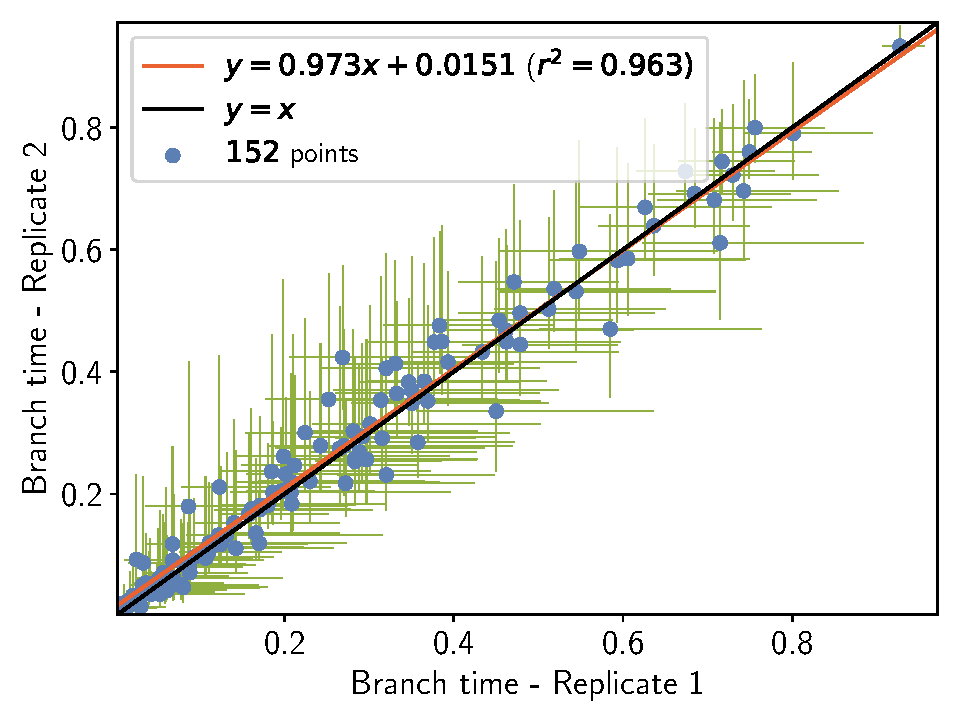
\includegraphics[width=\linewidth, page=1]{mammals/18CDS_SiteMutSelBranchNe_Rep_BranchTime-1-2}
		\end{minipage} \hfill
		\begin{minipage}{0.32\linewidth}
			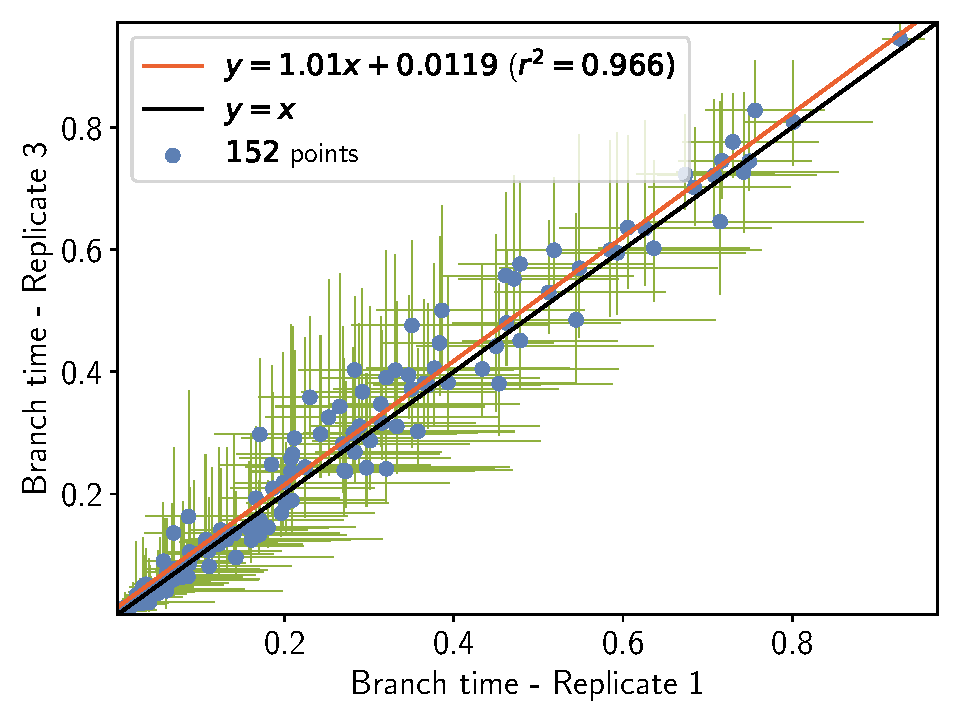
\includegraphics[width=\linewidth, page=1]{mammals/18CDS_SiteMutSelBranchNe_Rep_BranchTime-1-3}
		\end{minipage} \hfill
		\begin{minipage}{0.32\linewidth}
			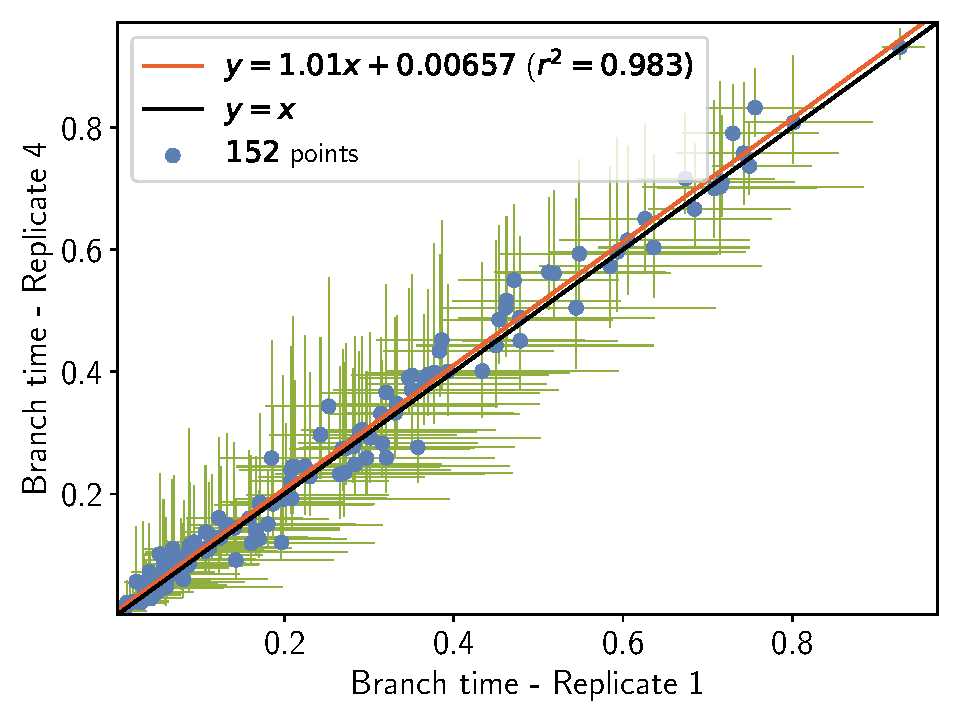
\includegraphics[width=\linewidth, page=1]{mammals/18CDS_SiteMutSelBranchNe_Rep_BranchTime-1-4}
		\end{minipage}
		\caption[Repeatability of branch time estimation in mammals]{Repeatability of branch time ($\Delta T$) estimation in mammals}
	\end{figure}

	\begin{table}[H]
		\centering
\noindent\adjustbox{max width=\textwidth}{%
\begin{tabu}{|c||c|c|c|}
\hline
\textbf{Correlation ($\bm{\rho}$)} & $\bm{N_{\mathrm{e}}}$ & $\bm{\mu}$ & \textbf{LogGenomeSize}\\
\hhline{|=#=|=|=|}
$\bm{N_{\mathrm{e}}}$ & - & $-0.0623$ & $-0.144$\\\hline
$\bm{\mu}$ & - & - & $0.224$\\\hline
\textbf{LogGenomeSize} & - & - & -\\\hline
\end{tabu}}
 \\
		\centering
\noindent\adjustbox{max width=\textwidth}{%
\begin{tabu}{|c||c|c|c|c|c|}
\hline
\textbf{Correlation ($\bm{\rho}$)} & $\bm{N_{\mathrm{e}}}$ & $\bm{\mu}$ & \textbf{Maximum longevity } & \textbf{Adult weight } & \textbf{Female maturity }\\
\hhline{|=#=|=|=|=|=|}
$\bm{N_{\mathrm{e}}}$ & - & $0.51^{**}$ & $-0.591^{**}$ & $-0.496^{**}$ & $-0.465^{**}$\\\hline
$\bm{\mu}$ & - & - & $-0.771^{**}$ & $-0.722^{**}$ & $-0.679^{**}$\\\hline
\textbf{Maximum longevity } & - & - & - & $0.802^{**}$ & $0.812^{**}$\\\hline
\textbf{Adult weight } & - & - & - & - & $0.764^{**}$\\\hline
\textbf{Female maturity } & - & - & - & - & -\\\hline
\end{tabu}}
 \\
		\centering
\noindent\adjustbox{max width=\textwidth}{%
\begin{tabu}{|c||c|c|c|}
\hline
\textbf{Correlation ($\bm{\rho}$)} & $\bm{N_{\mathrm{e}}}$ & $\bm{\mu}$ & \textbf{LogGenomeSize}\\
\hhline{|=#=|=|=|}
$\bm{N_{\mathrm{e}}}$ & - & $0.0479$ & $-0.158$\\\hline
$\bm{\mu}$ & - & - & $0.173$\\\hline
\textbf{LogGenomeSize} & - & - & -\\\hline
\end{tabu}}
 \\
		\centering
\noindent\adjustbox{max width=\textwidth}{%
\begin{tabu}{|c||c|c|c|}
\hline
\textbf{Correlation ($\bm{\rho}$)} & $\bm{N_{\mathrm{e}}}$ & $\bm{\mu}$ & \textbf{LogGenomeSize}\\
\hhline{|=#=|=|=|}
$\bm{N_{\mathrm{e}}}$ & - & $-0.0355$ & $-0.0875$\\\hline
$\bm{\mu}$ & - & - & $0.225$\\\hline
\textbf{LogGenomeSize} & - & - & -\\\hline
\end{tabu}}

		\caption[Covariance matrix repeatability in mammals]{
		In all four replicates, covariance coefficient between effective population size~($\Ne$), mutation rate per site per unit of time~($\mu$), and life-history traits (maximum longevity, adult weight and female maturity) were computed in placental mammals.
		Asterisks indicate strength of support ($\smash{^{*}} pp > 0.95$, $\smash{^{**}} pp > 0.975$).}
	\end{table}

	\subsection{Amino-acid preferences entropy}

	\begin{table}[H]
		\centering
		\noindent\adjustbox{max width=\textwidth}{%
		\begin{tabu}{|c|c|c|}
			\hline
			\textbf{Experiment} & $\left\langle \entropy \right\rangle$ (\textbf{branch} $\Ne$) & $\left\langle \entropy \right\rangle$ (\textbf{constant} $\Ne$) \\ \hline
			\hline
			Mammals 18 {CDS}, replicate~1, Chain 1 & $1.07 \pm 0.10$ & $1.14 \pm 0.10$\\ \hline
			Mammals 18 {CDS}, replicate 2, Chain 2 & $1.07 \pm 0.09$ & $1.14 \pm 0.10$\\ \hline
			Mammals 18 {CDS}, replicate 2, Chain 1 & $1.06 \pm 0.10$ & $1.12 \pm 0.09$\\ \hline
			Mammals 18 {CDS}, replicate 2, Chain 2 & $1.06 \pm 0.09$ & $1.11 \pm 0.10$\\ \hline
			Mammals 18 {CDS}, replicate 3, Chain 1 & $1.08 \pm 0.12$ & $1.15 \pm 0.11$\\ \hline
			Mammals 18 {CDS}, replicate 3, Chain 2 & $1.04 \pm 0.10$ & $1.18 \pm 0.11$\\ \hline
			Mammals 18 {CDS}, replicate 4, Chain 1 & $0.94 \pm 0.11$ & $1.02 \pm 0.12$\\ \hline
			Mammals 18 {CDS}, replicate 4, Chain 2 & $0.89 \pm 0.11$ & $1.02 \pm 0.11$\\ \hline
			\hline
			Mammals 36 {CDS}, replicate~1, Chain 1 & $1.02 \pm 0.06$ & $1.07 \pm 0.10$\\ \hline
			Mammals 36 {CDS}, replicate~1, Chain 2 & $0.91 \pm 0.07$ & $1.03 \pm 0.07$\\ \hline
			Mammals 36 {CDS}, replicate 2, Chain 1 & $0.92 \pm 0.09$ & $0.96 \pm 0.09$\\ \hline
			Mammals 36 {CDS}, replicate 2, Chain 2 & $1.01 \pm 0.09$ & $1.02 \pm 0.11$\\ \hline
			Mammals 36 {CDS}, replicate 3, Chain 1 & $0.93 \pm 0.00$ & $1.05 \pm 0.09$\\ \hline
			Mammals 36 {CDS}, replicate 3, Chain 2 & $1.02 \pm 0.07$ & $1.05 \pm 0.11$\\ \hline
			Mammals 36 {CDS}, replicate 4, Chain 1 & $1.04 \pm 0.07$ & $1.10 \pm 0.08$\\ \hline
			Mammals 36 {CDS}, replicate 4, Chain 2 & $1.03 \pm 0.10$ & $1.08 \pm 0.08$\\ \hline
			Mammals 36 {CDS}, replicate 5, Chain 1 & $1.03 \pm 0.10$ & $1.03 \pm 0.08$\\ \hline
			Mammals 36 {CDS}, replicate 5, Chain 2 & $0.99 \pm 0.10$ & $1.04 \pm 0.08$\\ \hline
			Mammals 36 {CDS}, replicate 6, Chain 1 & $1.05 \pm 0.10$ & $1.10 \pm 0.08$\\ \hline
			Mammals 36 {CDS}, replicate 6, Chain 2 & $0.97 \pm 0.11$ & $1.10 \pm 0.10$\\ \hline
		\end{tabu}}
		\caption[Entropy of amino acids in mammals]{Estimated amino-acid entropy in mammals.
		Obtained with the mechanistic inference model developed in this paper of site-specific amino-acid fitness profiles and log-Brownian process for $\Ne$, $\mu$ and life-history traits (in the left column), or under the assumption of constant $\Ne$ (in the right column).}
		\label{tab:table-entropy-aa-mutselne}
	\end{table}

	\subsection{Traits estimation with branch \texorpdfstring{$\omega$}{ω} (replicate~1, chain~1)}
	Obtained with the phenomenological inference model of log-Brownian process for the $\mu$ and the relative {non-synonymous} {substitution} rate ($\omega$), as in \citet{Lartillot2011}.

	\begin{figure}[H]
		\centering
		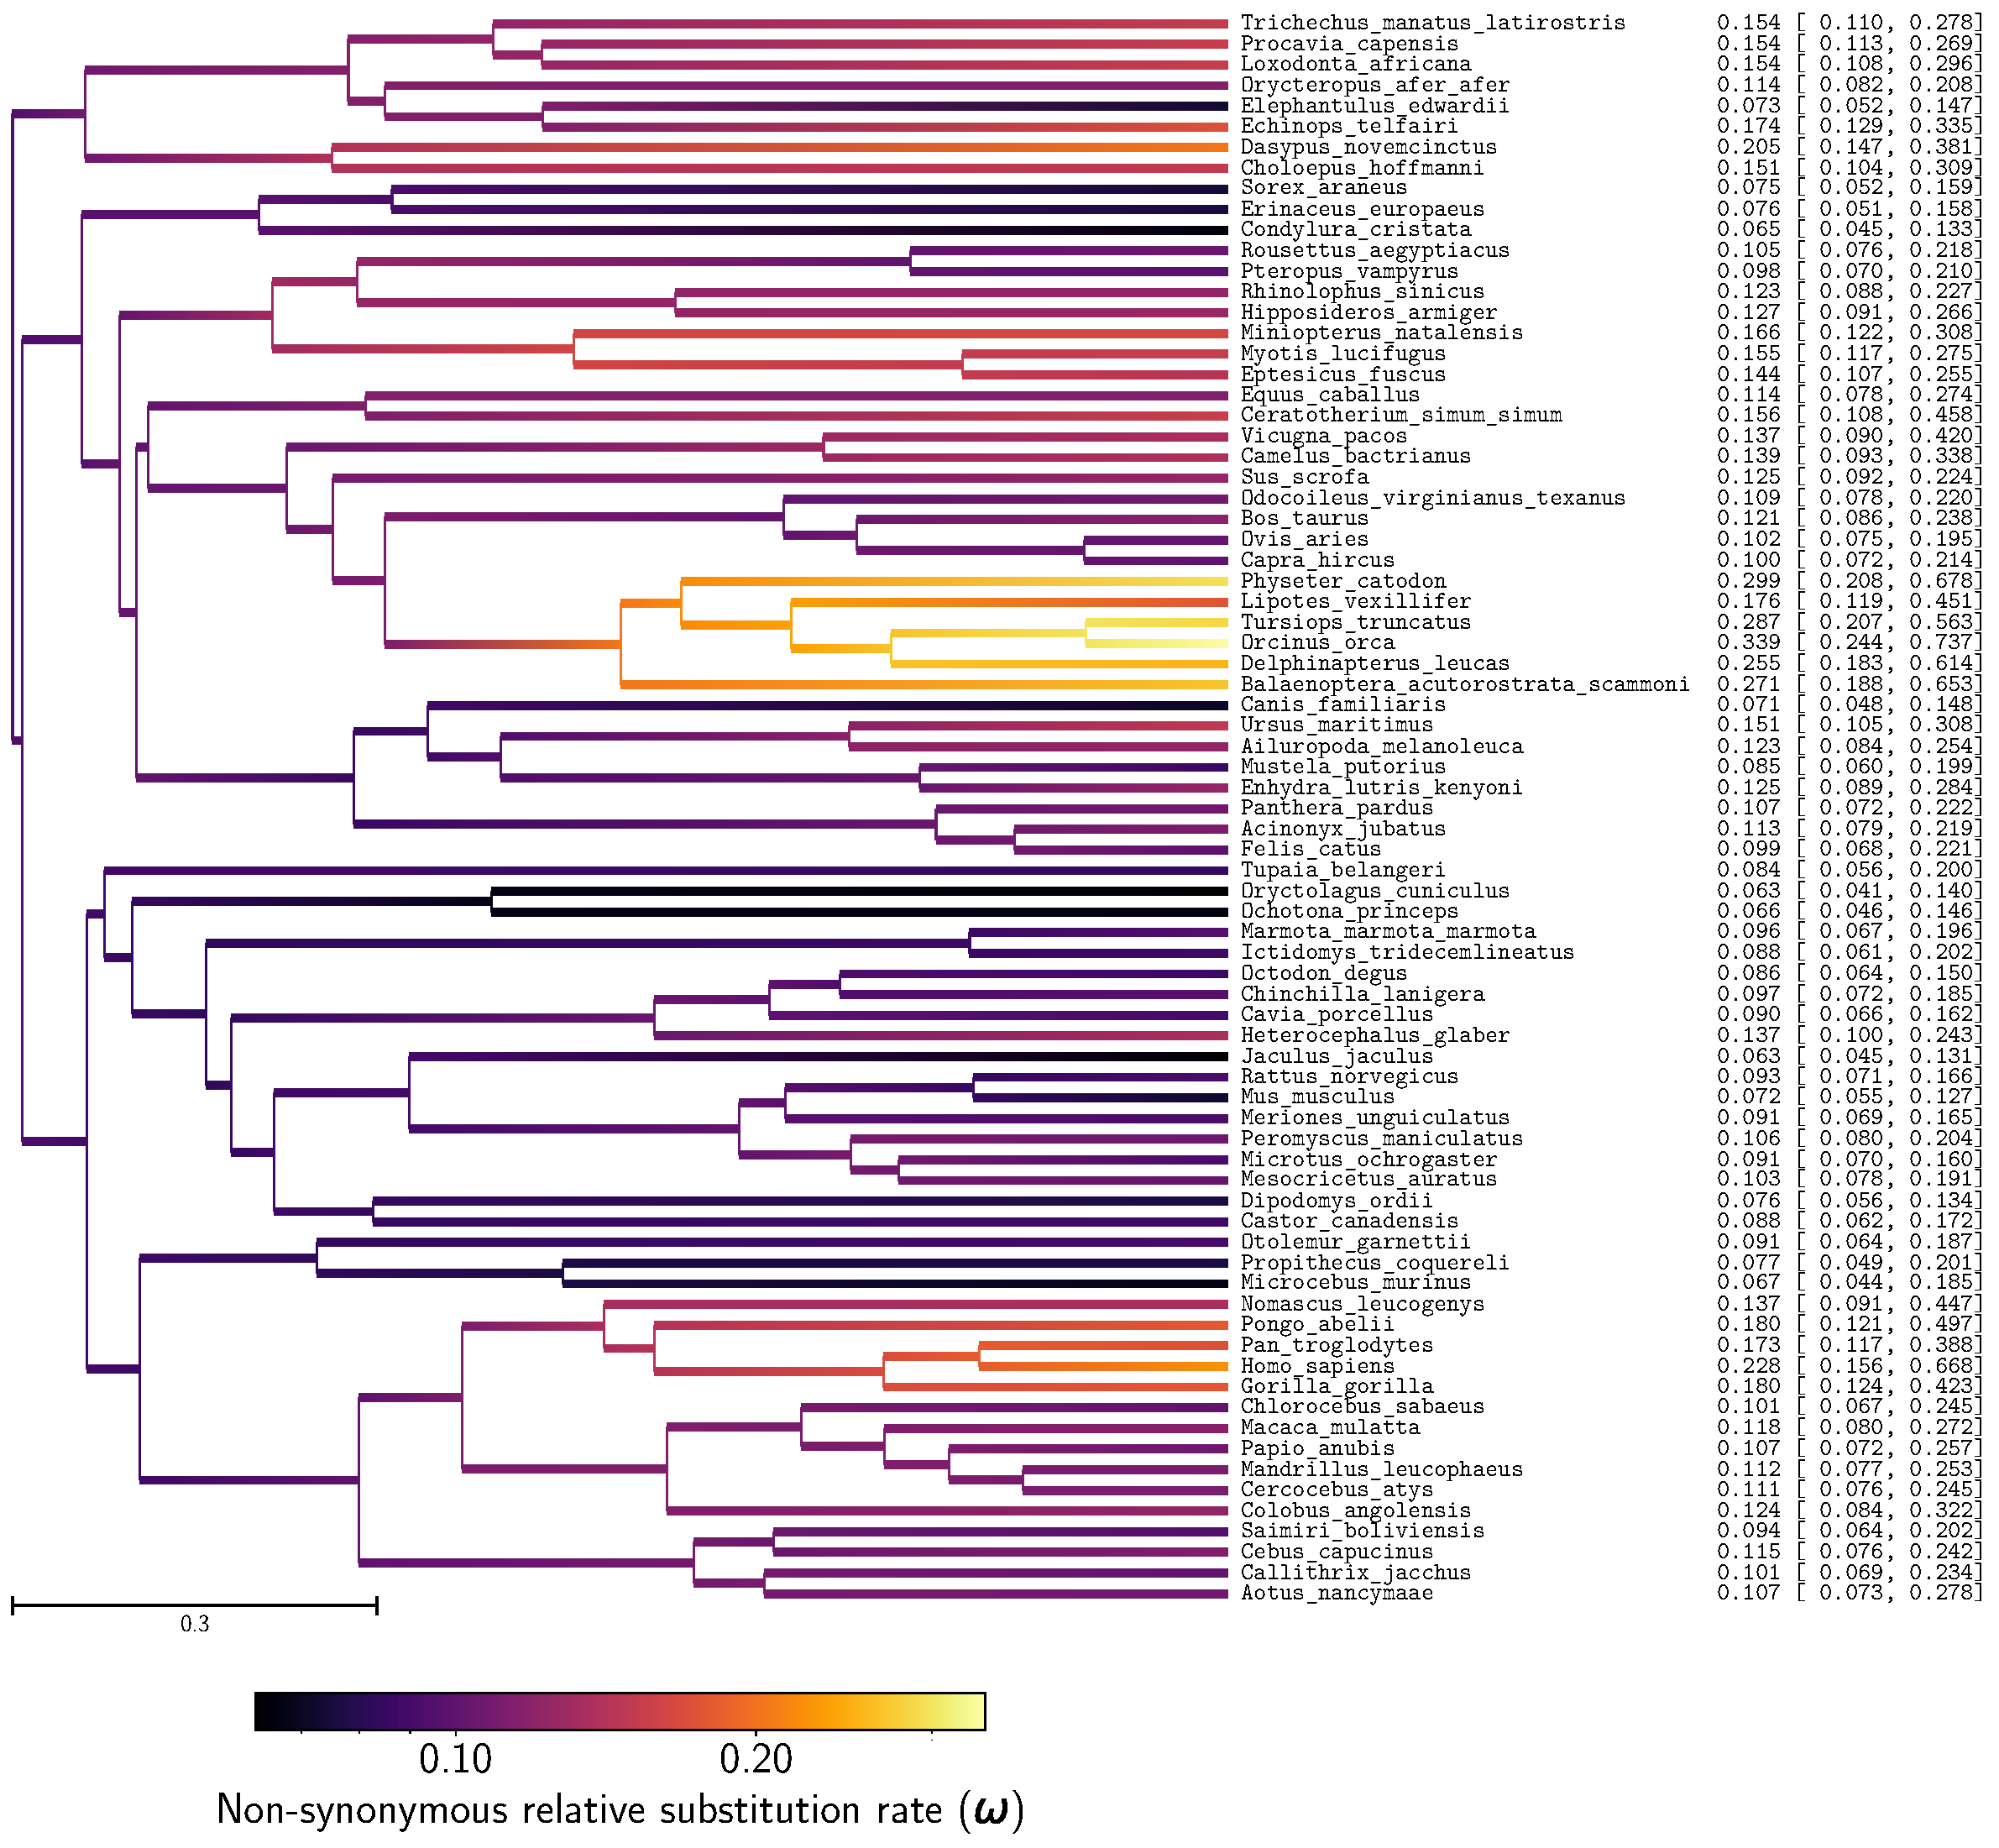
\includegraphics[width=\linewidth, page=1]{mammals/18CDS_BranchOmega_R1_LogdNdS}
		\caption[$\omega$ estimation in mammals]{{Non-synonymous substitution} rate ($\omega$) estimation in mammals}
	\end{figure}

	\begin{table}[H]
		\centering
\noindent\adjustbox{max width=\textwidth}{%
\begin{tabu}{|c||c|c|c|}
\hline
\textbf{Correlation ($\bm{\rho}$)} & $\bm{\omega}$ & $\bm{\mu}$ & \textbf{LogGenomeSize}\\
\hhline{|=#=|=|=|}
$\bm{\omega}$ & - & $0.147$ & $0.152$\\\hline
$\bm{\mu}$ & - & - & $0.251$\\\hline
\textbf{LogGenomeSize} & - & - & -\\\hline
\end{tabu}}

		\caption[Correlation coefficient matrix in mammals ($\omega$)]{
		Correlation coefficient between {non-synonymous} {substitution} rate~($\omega$), mutation rate per site per unit of time~($\mu$), and life-history traits (maximum longevity, adult weight and female maturity) were computed in placental mammals.
		Asterisks indicate strength of support ($\smash{^{*}} pp > 0.95$, $\smash{^{**}} pp > 0.975$).}
	\end{table}

	\begin{table}[H]
		\centering
\noindent\adjustbox{max width=\textwidth}{%
\begin{tabu}{|c||c|c|c|c|c|}
\hline
\textbf{Covariance ($\bm{\Sigma}$)} & $\bm{\omega}$ & $\bm{\mu}$ & \textbf{Maximum longevity } & \textbf{Adult weight } & \textbf{Female maturity }\\
\hhline{|=#=|=|=|=|=|}
$\bm{\omega}$ & $0.215^{**}$ & $-0.236^{**}$ & $0.231^{**}$ & $0.828^{**}$ & $0.242^{**}$\\\hline
$\bm{\mu}$ & - & $1.82^{**}$ & $-0.998^{**}$ & $-4.38^{**}$ & $-1.34^{**}$\\\hline
\textbf{Maximum longevity } & - & - & $0.837^{**}$ & $3.04^{**}$ & $0.917^{**}$\\\hline
\textbf{Adult weight } & - & - & - & $17.1^{**}$ & $3.93^{**}$\\\hline
\textbf{Female maturity } & - & - & - & - & $1.45^{**}$\\\hline
\end{tabu}}

		\caption[Covariance matrix in mammals ($\omega$)]{
		Correlation coefficient between {non-synonymous} {substitution} rate~($\omega$), mutation rate per site per unit of time~($\mu$), and life-history traits (maximum longevity, adult weight and female maturity) were computed in placental mammals.
		Asterisks indicate strength of support ($\smash{^{*}} pp > 0.95$, $\smash{^{**}} pp > 0.975$).}
	\end{table}

	\begin{table}[H]
		\centering
\noindent\adjustbox{max width=\textwidth}{%
\begin{tabu}{|c||c|c|c|c|c|}
\hline
\textbf{Partial coefficient} & $\bm{\omega}$ & $\bm{\mu}$ & \textbf{Maximum longevity } & \textbf{Adult weight } & \textbf{Female maturity }\\
\hhline{|=#=|=|=|=|=|}
$\bm{\omega}$ & - & $0.15$ & $0.369^{**}$ & $0.0468$ & $0.0223$\\\hline
$\bm{\mu}$ & - & - & $-0.299^{*}$ & $-0.272$ & $-0.382^{**}$\\\hline
\textbf{Maximum longevity } & - & - & - & $0.283^{**}$ & $0.338^{**}$\\\hline
\textbf{Adult weight } & - & - & - & - & $0.21^{*}$\\\hline
\textbf{Female maturity } & - & - & - & - & -\\\hline
\end{tabu}}

		\caption[Partial correlation coefficient matrix in mammals ($\omega$)]{
		Partial correlation coefficient between {non-synonymous} {substitution} rate~($\omega$), mutation rate per site per unit of time~($\mu$), and life-history traits (maximum longevity, adult weight and female maturity) were computed in placental mammals.
		Asterisks indicate strength of support ($\smash{^{*}} pp > 0.95$, $\smash{^{**}} pp > 0.975$).}
	\end{table}


	\section{Empirical data in Isopods}
	\label{sec:empirical-data-in-isopods}

	\subsection{Traits estimation (replicate~1, chain~1)}
	Obtained with the mechanistic inference model developed in this paper of site-specific amino-acid fitness profiles and log-Brownian process for $\Ne$, $\mu$ and life-history traits.

	\begin{figure}[H]
		\centering
		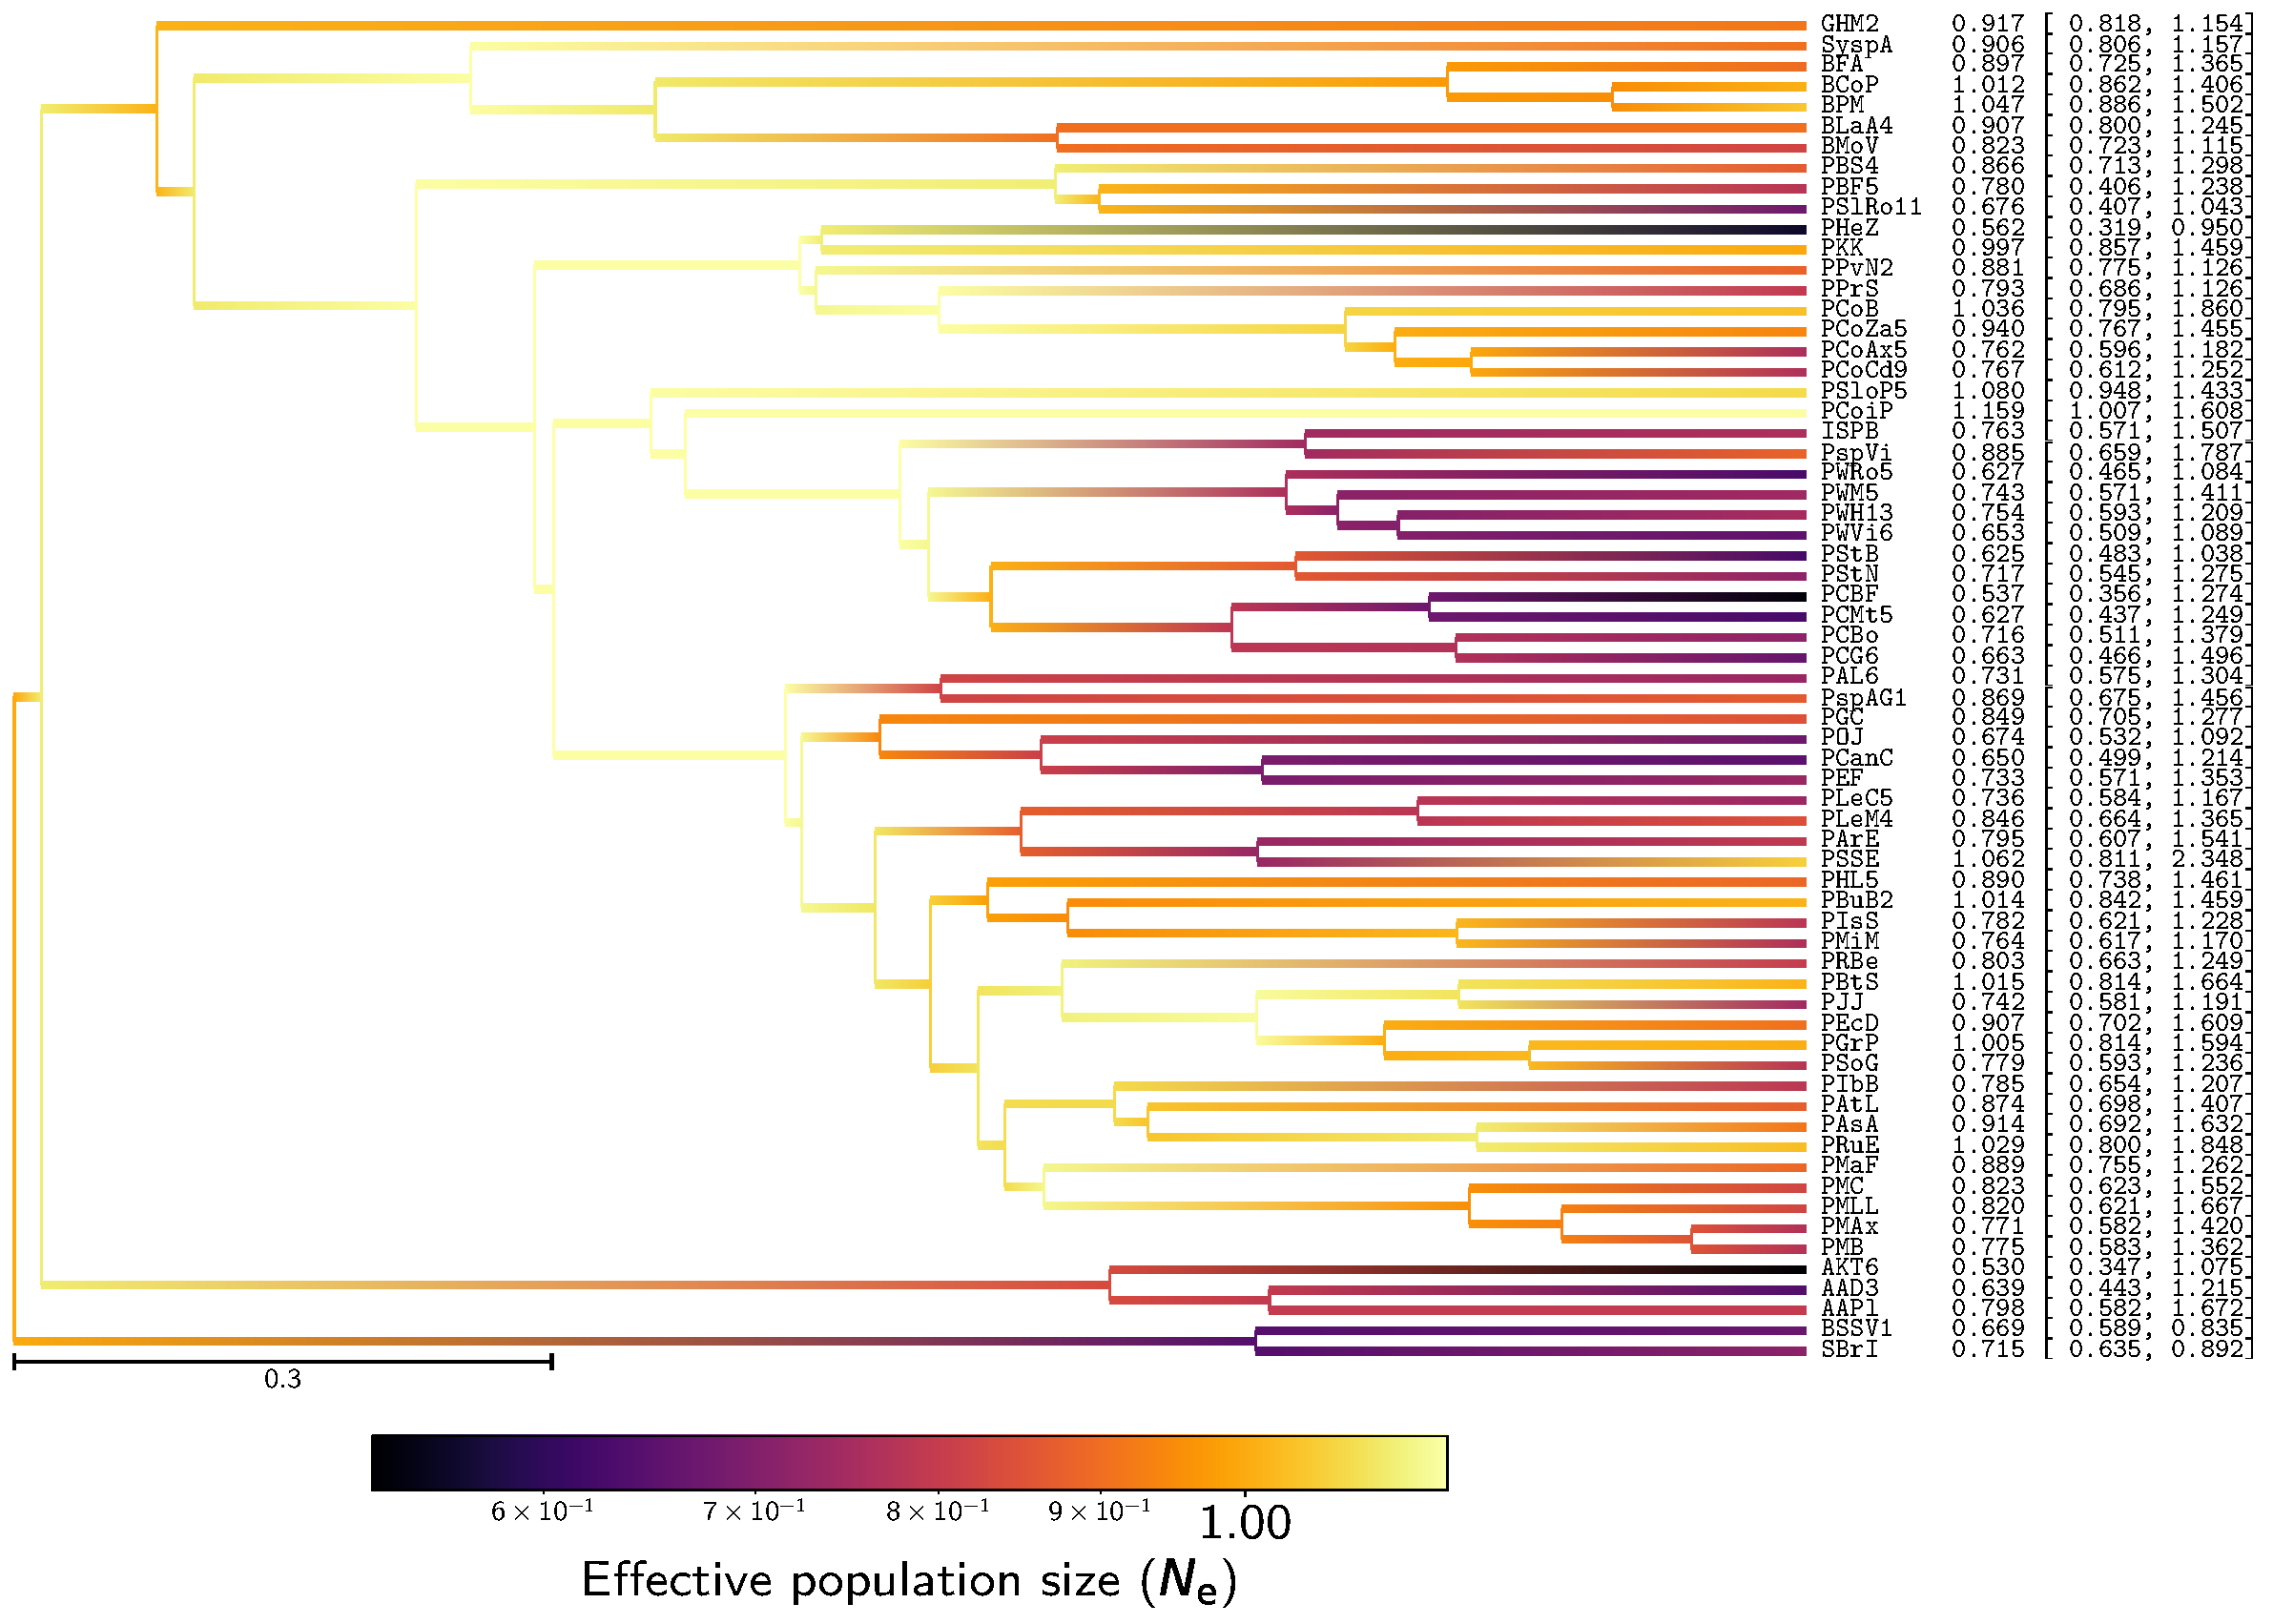
\includegraphics[width=\linewidth, page=1]{isopods/12CDS_SiteMutSelBranchNe_R1_LogPopulationSize}
		\caption[$\Ne$ estimation in isopods]{Effective population size ($\Ne$) estimation in isopods}
	\end{figure}

	\begin{figure}[H]
		\centering
		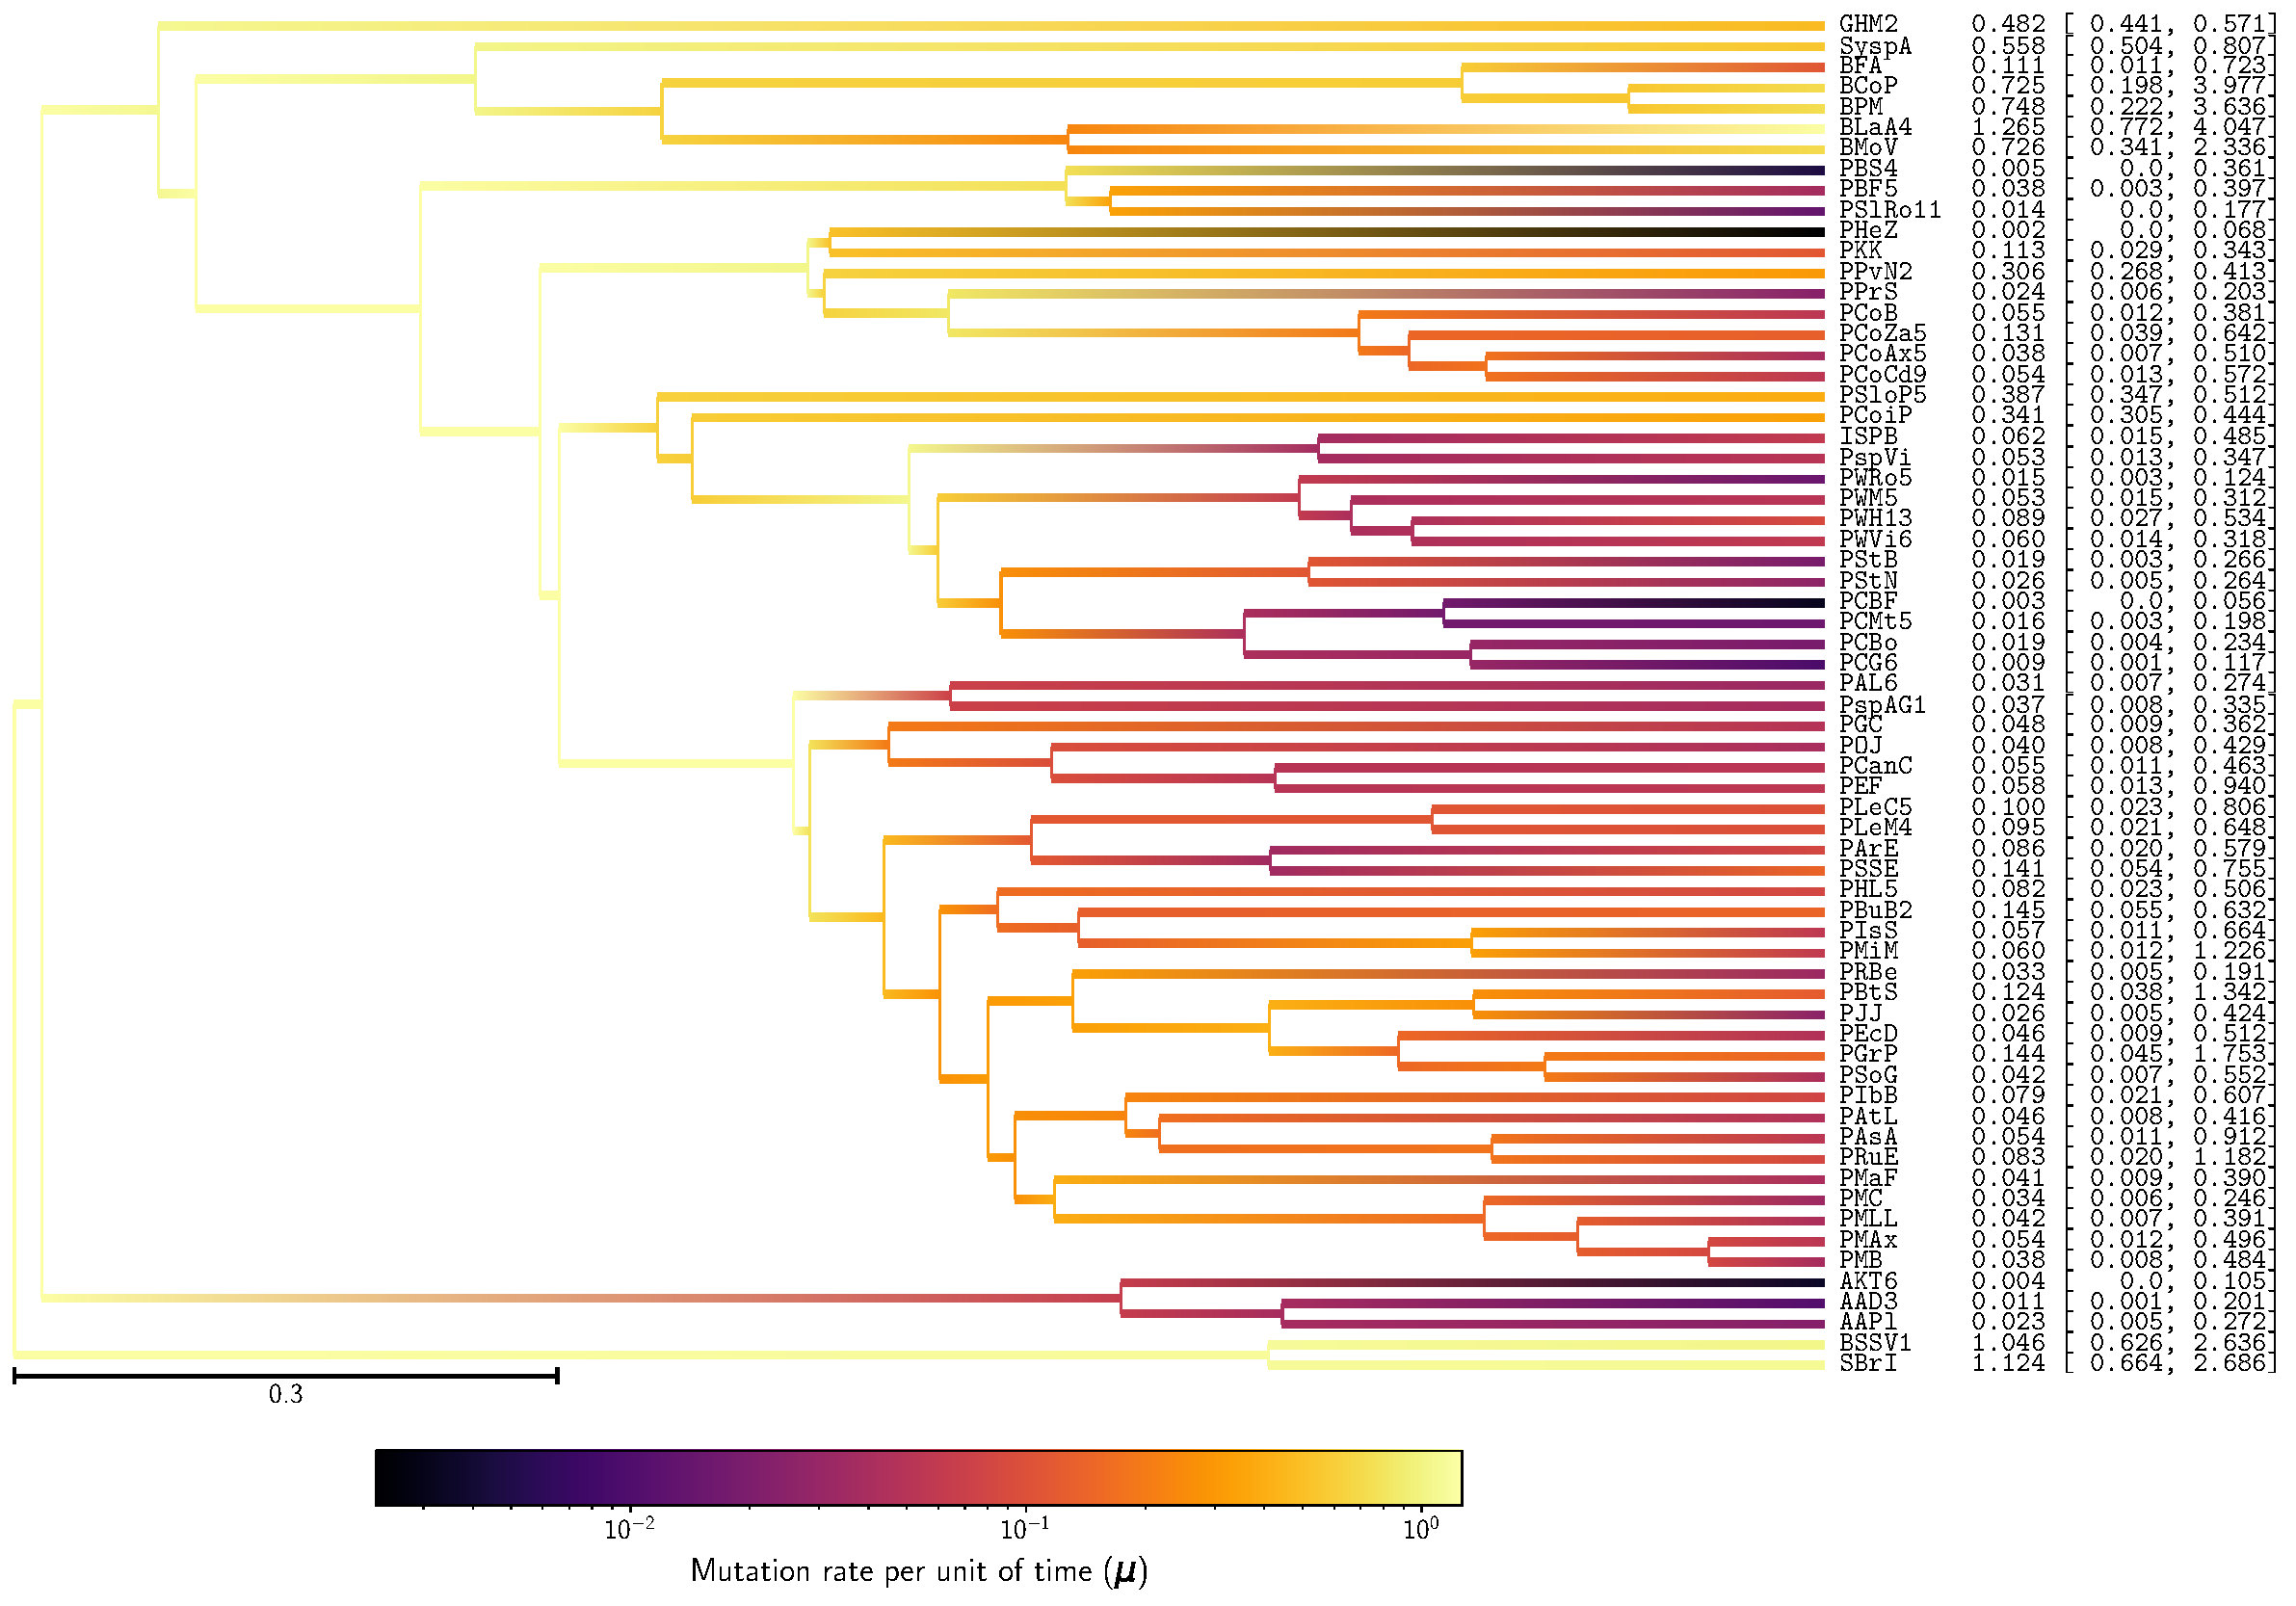
\includegraphics[width=\linewidth, page=1]{isopods/12CDS_SiteMutSelBranchNe_R1_LogMutationRatePerTime}
		\caption[Mutation rate estimation in isopods]{Mutation rate ($\mu$) estimation in isopods}
	\end{figure}

	\subsection{Repeatability of experiments}
	\label{subsec:repeatability-of-experiments-isopods}
	$6$ independent inferences were performed on a randomly chosen set of $12$ coding sequences ({CDS}) out of $135$.
	Obtained with the mechanistic inference model developed in this paper of site-specific amino-acid fitness profiles and log-Brownian process for $\Ne$, $\mu$.
	Each plot is a correlation between a pair of experiments for a given parameter.
	For each node (or branch) of the tree, the mean {posterior} of the parameter over the {MCMC} (after burn-in) is represented in blue dots, green solid lines are the $90\%$ confidence interval of the {MCMC}.
	Solid red line is the regression line between replicates.

	\begin{figure}[H]
		\centering
		\begin{minipage}{0.32\linewidth}
			\includegraphics[width=\linewidth, page=1]{isopods/12CDS_SiteMutSelBranchNe_Rep-1-2_Log10BranchLength}
		\end{minipage} \hfill
		\begin{minipage}{0.32\linewidth}
			\includegraphics[width=\linewidth, page=1]{isopods/12CDS_SiteMutSelBranchNe_Rep-1-3_Log10BranchLength}
		\end{minipage} \hfill
		\begin{minipage}{0.32\linewidth}
			\includegraphics[width=\linewidth, page=1]{isopods/12CDS_SiteMutSelBranchNe_Rep-1-4_Log10BranchLength}
		\end{minipage}
		\begin{minipage}{0.32\linewidth}
			\includegraphics[width=\linewidth, page=1]{isopods/12CDS_SiteMutSelBranchNe_Rep-1-5_Log10BranchLength}
		\end{minipage}
		\begin{minipage}{0.32\linewidth}
			\includegraphics[width=\linewidth, page=1]{isopods/12CDS_SiteMutSelBranchNe_Rep-1-6_Log10BranchLength}
		\end{minipage}
		\caption[Repeatability of branch length estimation in isopods]{Repeatability of branch length ($\branchlength$) estimation in isopods}
	\end{figure}

	\begin{figure}[H]
		\centering
		\begin{minipage}{0.32\linewidth}
			\includegraphics[width=\linewidth, page=1]{isopods/12CDS_SiteMutSelBranchNe_Rep-1-2_LogPopulationSize}
		\end{minipage} \hfill
		\begin{minipage}{0.32\linewidth}
			\includegraphics[width=\linewidth, page=1]{isopods/12CDS_SiteMutSelBranchNe_Rep-1-3_LogPopulationSize}
		\end{minipage} \hfill
		\begin{minipage}{0.32\linewidth}
			\includegraphics[width=\linewidth, page=1]{isopods/12CDS_SiteMutSelBranchNe_Rep-1-4_LogPopulationSize}
		\end{minipage}
		\begin{minipage}{0.32\linewidth}
			\includegraphics[width=\linewidth, page=1]{isopods/12CDS_SiteMutSelBranchNe_Rep-1-5_LogPopulationSize}
		\end{minipage}
		\begin{minipage}{0.32\linewidth}
			\includegraphics[width=\linewidth, page=1]{isopods/12CDS_SiteMutSelBranchNe_Rep-1-6_LogPopulationSize}
		\end{minipage}
		\caption[Repeatability of $\Ne$ estimation in isopods]{Repeatability of {effective population size} ($\Ne$) estimation in isopods}
	\end{figure}

	\begin{table}[htbp]
		\renewcommand{\arraystretch}{0.5}
		\scriptsize
		\noindent\adjustbox{max width=\textwidth}{%
		\begin{tabular}{lllllllllll}
\toprule
         Rep. 1 &          Rep. 2 &          Rep. 3 &          Rep. 4 &          Rep. 5 &          Rep. 6 &      Habitat & Pigmentation & Ocular structure &     Code &                                    Taxon \\
\midrule
          0.917 &            1.21 &            0.91 &            1.09 &             1.1 &           0.997 &  Underground &  Depigmented &     Anophthalmia &     GHM2 &               \textit{Gallasellus heyli} \\
          0.906 &           0.511 &           0.876 &           0.907 &           0.948 &           0.964 &  Underground &  Depigmented &     Anophthalmia &    SyspA &                   \textit{Synasellus sp} \\
          0.897 &           0.954 &           0.838 &           0.819 &           0.721 &           0.859 &  Underground &  Depigmented &     Anophthalmia &      BFA &          \textit{Bragasellus frontellum} \\
           1.01 &            1.15 &            0.78 &           0.894 &            0.78 &           0.945 &      Surface &    Pigmented &           Ocular &     BCoP &             \textit{Bragasellus cortesi} \\
           1.05 &            0.95 &           0.881 &           0.815 &            0.87 &            1.08 &      Surface &    Pigmented &           Ocular &      BPM &            \textit{Bragasellus peltatus} \\
          0.907 &           0.891 &           0.769 &           0.831 &           0.873 &           0.907 &  Underground &  Depigmented &     Anophthalmia &    BLaA4 &                               \textit{-} \\
          0.823 &           0.797 &           0.839 &           0.949 &           0.852 &            1.06 &  Underground &  Depigmented &     Anophthalmia &     BMoV &             \textit{Bragasellus molinai} \\
          0.866 &            0.39 &            0.61 &            0.51 &           0.773 &           0.871 &  Underground &  Depigmented &     Anophthalmia &     PBS4 &                 \textit{Proasellus boui} \\
           0.78 &           0.637 &           0.702 &           0.808 &           0.919 &           0.884 &  Underground &  Depigmented &     Anophthalmia &     PBF5 &                 \textit{Proasellus boui} \\
          0.676 &           0.657 &           0.718 &           0.895 &           0.777 &           0.884 &  Underground &  Depigmented &     Anophthalmia &  PSlRo11 &               \textit{Proasellus slavus} \\
          0.562 &           0.681 &            0.62 &           0.616 &           0.778 &           0.608 &  Underground &  Depigmented &     Anophthalmia &     PHeZ &      \textit{Proasellus hercegovinensis} \\
          0.997 &            1.15 &           0.962 &            1.08 &           0.907 &            1.06 &      Surface &    Pigmented &           Ocular &      PKK &             \textit{Proasellus karamani} \\
          0.881 &           0.897 &           0.753 &           0.746 &           0.877 &           0.901 &  Underground &  Depigmented &     Anophthalmia &    PPvN2 &               \textit{Proasellus pavani} \\
          0.793 &            0.66 &           0.876 &           0.711 &           0.813 &           0.808 &  Underground &  Depigmented &     Anophthalmia &     PPrS &             \textit{Proasellus parvulus} \\
           1.04 &            1.06 &            1.06 &           0.968 &            1.05 &           0.957 &      Surface &    Pigmented &           Ocular &     PCoB &              \textit{Proasellus coxalis} \\
           0.94 &            1.17 &            1.06 &           0.937 &            1.18 &            1.14 &      Surface &    Pigmented &           Ocular &   PCoZa5 &              \textit{Proasellus coxalis} \\
          0.762 &           0.595 &           0.792 &           0.731 &           0.902 &           0.657 &  Underground &  Depigmented &     Anophthalmia &   PCoAx5 &              \textit{Proasellus coxalis} \\
          0.767 &           0.705 &           0.711 &           0.848 &           0.847 &           0.761 &  Underground &  Depigmented &   Microphthalmia &   PCoCd9 &              \textit{Proasellus coxalis} \\
           1.08 &            1.09 &           0.893 &           0.975 &             1.1 &           0.968 &  Underground &  Depigmented &     Anophthalmia &   PSloP5 &           \textit{Proasellus slovenicus} \\
           1.16 &            1.28 &            1.02 &            1.07 &            1.21 &            1.32 &      Surface &    Pigmented &           Ocular &    PCoiP &            \textit{Proasellus coiffaiti} \\
          0.763 &           0.888 &           0.753 &           0.709 &           0.766 &            0.86 &  Underground &  Depigmented &     Anophthalmia &     ISPB &                  \textit{Proasellus nsp} \\
          0.885 &           0.789 &           0.765 &           0.675 &            0.67 &           0.857 &  Underground &  Depigmented &     Anophthalmia &    PspVi &                  \textit{Proasellus nsp} \\
          0.627 &           0.636 &           0.493 &           0.771 &           0.754 &           0.732 &  Underground &  Depigmented &     Anophthalmia &    PWRo5 &              \textit{Proasellus walteri} \\
          0.743 &           0.671 &           0.558 &            1.03 &           0.834 &           0.761 &  Underground &  Depigmented &     Anophthalmia &     PWM5 &              \textit{Proasellus walteri} \\
          0.754 &           0.718 &            0.54 &            0.79 &           0.656 &           0.824 &  Underground &  Depigmented &     Anophthalmia &    PWH13 &              \textit{Proasellus walteri} \\
          0.653 &           0.689 &           0.538 &           0.774 &           0.667 &           0.764 &  Underground &  Depigmented &     Anophthalmia &    PWVi6 &              \textit{Proasellus walteri} \\
          0.625 &           0.701 &           0.682 &           0.703 &           0.796 &           0.875 &  Underground &  Depigmented &     Anophthalmia &     PStB &            \textit{Proasellus strouhali} \\
          0.717 &           0.693 &           0.682 &           0.582 &           0.839 &           0.734 &  Underground &  Depigmented &     Anophthalmia &     PStN &            \textit{Proasellus strouhali} \\
          0.537 &           0.535 &           0.475 &           0.941 &           0.705 &           0.656 &  Underground &  Depigmented &     Anophthalmia &     PCBF &            \textit{Proasellus cavaticus} \\
          0.627 &           0.611 &           0.512 &           0.659 &           0.614 &            0.68 &  Underground &  Depigmented &     Anophthalmia &    PCMt5 &            \textit{Proasellus cavaticus} \\
          0.716 &           0.761 &           0.632 &           0.603 &           0.844 &           0.747 &  Underground &  Depigmented &     Anophthalmia &     PCBo &            \textit{Proasellus cavaticus} \\
          0.663 &           0.437 &           0.495 &           0.535 &           0.689 &           0.793 &  Underground &  Depigmented &     Anophthalmia &     PCG6 &            \textit{Proasellus cavaticus} \\
          0.731 &           0.668 &           0.778 &           0.805 &           0.608 &           0.568 &  Underground &  Depigmented &     Anophthalmia &     PAL6 &           \textit{Proasellus albigensis} \\
          0.869 &           0.737 &           0.729 &            0.92 &           0.827 &           0.896 &  Underground &  Depigmented &     Anophthalmia &   PspAG1 &                    \textit{Proasellus n} \\
          0.849 &           0.839 &            0.95 &           0.966 &           0.931 &            0.94 &  Underground &  Depigmented &     Anophthalmia &      PGC &                \textit{Proasellus grafi} \\
          0.674 &            0.79 &           0.719 &           0.772 &           0.784 &           0.826 &      Surface &   Part. dep. &   Microphthalmia &      POJ &               \textit{Proasellus ortizi} \\
           0.65 &           0.517 &           0.732 &           0.613 &           0.711 &           0.729 &  Underground &  Depigmented &     Anophthalmia &    PCanC &          \textit{Proasellus cantabricus} \\
          0.733 &           0.659 &           0.684 &           0.579 &           0.795 &           0.802 &      Surface &   Part. dep. &   Microphthalmia &      PEF &             \textit{Proasellus ebrensis} \\
          0.736 &           0.743 &             0.8 &           0.685 &           0.805 &           0.935 &  Underground &  Depigmented &     Anophthalmia &    PLeC5 &                               \textit{-} \\
          0.846 &           0.711 &           0.785 &           0.864 &           0.957 &           0.889 &  Underground &  Depigmented &     Anophthalmia &    PLeM4 &                               \textit{-} \\
          0.795 &            1.03 &           0.846 &            0.87 &           0.869 &           0.851 &      Surface &   Part. dep. &   Microphthalmia &     PArE &          \textit{Proasellus aragonensis} \\
           1.06 &           0.785 &           0.694 &           0.756 &           0.893 &           0.804 &  Underground &  Depigmented &     Anophthalmia &     PSSE &             \textit{Proasellus spelaeus} \\
           0.89 &           0.774 &           0.727 &           0.766 &           0.926 &           0.992 &  Underground &  Depigmented &     Anophthalmia &     PHL5 &                               \textit{-} \\
           1.01 &           0.994 &           0.783 &           0.789 &            1.14 &            1.17 &  Underground &  Depigmented &     Anophthalmia &    PBuB2 &                               \textit{-} \\
          0.782 &            1.14 &           0.991 &           0.853 &               1 &            1.07 &      Surface &    Pigmented &           Ocular &     PIsS &            \textit{Proasellus istrianus} \\
          0.764 &           0.878 &           0.853 &           0.736 &           0.887 &           0.966 &      Surface &    Pigmented &           Ocular &     PMiM &      \textit{Proasellus micropectinatus} \\
          0.803 &            1.08 &           0.819 &            0.96 &             1.1 &           0.823 &      Surface &   Part. dep. &   Microphthalmia &     PRBe &           \textit{Proasellus racovitzai} \\
           1.01 &             1.1 &           0.905 &           0.931 &           0.884 &            1.01 &      Surface &    Pigmented &           Ocular &     PBtS &              \textit{Proasellus beticus} \\
          0.742 &           0.896 &           0.842 &           0.826 &            0.84 &           0.882 &  Underground &  Depigmented &   Microphthalmia &      PJJ &           \textit{Proasellus jaloniacus} \\
          0.907 &            1.04 &           0.792 &           0.594 &           0.859 &           0.836 &  Underground &  Depigmented &     Anophthalmia &     PEcD &              \textit{Proasellus escolai} \\
           1.01 &            1.02 &            0.86 &           0.786 &            1.06 &           0.922 &      Surface &   Part. dep. &   Microphthalmia &     PGrP &          \textit{Proasellus granadensis} \\
          0.779 &           0.738 &           0.707 &           0.731 &           0.812 &           0.808 &  Underground &  Depigmented &     Anophthalmia &     PSoG &             \textit{Proasellus solanasi} \\
          0.785 &           0.918 &           0.854 &           0.788 &            1.04 &           0.986 &      Surface &    Pigmented &           Ocular &     PIbB &             \textit{Proasellus ibericus} \\
          0.874 &           0.836 &           0.764 &           0.815 &           0.866 &            1.05 &  Underground &  Depigmented &     Anophthalmia &     PAtL &          \textit{Proasellus arthrodilus} \\
          0.914 &           0.951 &           0.888 &           0.834 &           0.881 &           0.886 &      Surface &   Part. dep. &   Microphthalmia &     PAsA &         \textit{Proasellus assaforensis} \\
           1.03 &           0.994 &           0.939 &           0.854 &           0.971 &               1 &  Underground &  Depigmented &     Anophthalmia &     PRuE &               \textit{Proasellus rectus} \\
          0.889 &           0.764 &           0.761 &           0.651 &           0.698 &           0.847 &  Underground &  Depigmented &     Anophthalmia &     PMaF &            \textit{Proasellus margalefi} \\
          0.823 &             1.1 &           0.961 &           0.914 &            1.03 &           0.838 &      Surface &    Pigmented &           Ocular &      PMC &           \textit{Proasellus meridianus} \\
           0.82 &            1.05 &           0.806 &           0.914 &           0.856 &           0.799 &      Surface &    Pigmented &           Ocular &     PMLL &           \textit{Proasellus meridianus} \\
          0.771 &           0.889 &           0.796 &           0.907 &           0.839 &           0.863 &  Underground &   Part. dep. &   Microphthalmia &     PMAx &           \textit{Proasellus meridianus} \\
          0.775 &           0.982 &           0.892 &            1.02 &            1.05 &           0.882 &      Surface &    Pigmented &           Ocular &      PMB &           \textit{Proasellus meridianus} \\
           0.53 &            0.57 &            0.71 &           0.679 &           0.413 &           0.603 &  Underground &  Depigmented &     Anophthalmia &     AKT6 &                \textit{Asellus kosswigi} \\
          0.639 &           0.936 &           0.732 &           0.859 &           0.859 &           0.866 &      Surface &    Pigmented &           Ocular &     AAD3 &               \textit{Asellus aquaticus} \\
          0.798 &           0.882 &           0.795 &            0.89 &           0.641 &           0.875 &      Surface &    Pigmented &           Ocular &     AAPl &               \textit{Asellus aquaticus} \\
          0.669 &           0.704 &           0.684 &           0.655 &           0.805 &           0.711 &  Underground &  Depigmented &     Anophthalmia &    BSSV1 &  \textit{Balkanostenasellus skopljensis} \\
          0.715 &           0.682 &           0.685 &           0.614 &           0.707 &            0.77 &  Underground &  Depigmented &     Anophthalmia &     SBrI &             \textit{Stenasellus breuili} \\
 \textbf{ 2.19} &  \textbf{ 3.29} &  \textbf{ 2.24} &  \textbf{ 2.13} &  \textbf{ 2.93} &  \textbf{ 2.33} &            - &            - &                - &        - &                   \textbf{Maximum range} \\
\bottomrule
\end{tabular}

		}
		\caption[Repeatability of $\Ne$ estimation in isopods]{Repeatability of {effective population size} ($\Ne$) estimation in isopods, for the extant taxa.}
		\label{tab:Ne-estimated-isopods}
	\end{table}

	\begin{figure}[H]
		\centering
		\begin{minipage}{0.32\linewidth}
			\includegraphics[width=\linewidth, page=1]{isopods/12CDS_SiteMutSelBranchNe_Rep-1-2_LogMutationRatePerTime}
		\end{minipage} \hfill
		\begin{minipage}{0.32\linewidth}
			\includegraphics[width=\linewidth, page=1]{isopods/12CDS_SiteMutSelBranchNe_Rep-1-3_LogMutationRatePerTime}
		\end{minipage} \hfill
		\begin{minipage}{0.32\linewidth}
			\includegraphics[width=\linewidth, page=1]{isopods/12CDS_SiteMutSelBranchNe_Rep-1-4_LogMutationRatePerTime}
		\end{minipage}
		\begin{minipage}{0.32\linewidth}
			\includegraphics[width=\linewidth, page=1]{isopods/12CDS_SiteMutSelBranchNe_Rep-1-5_LogMutationRatePerTime}
		\end{minipage}
		\begin{minipage}{0.32\linewidth}
			\includegraphics[width=\linewidth, page=1]{isopods/12CDS_SiteMutSelBranchNe_Rep-1-6_LogMutationRatePerTime}
		\end{minipage}
		\caption[Repeatability of $\mu$ estimation in isopods]{Repeatability of mutation rate ($\mu$) estimation in isopods}
	\end{figure}

	\begin{table}[htbp]
		\renewcommand{\arraystretch}{0.5}
		\scriptsize
		\noindent\adjustbox{max width=\textwidth}{%
		\begin{tabular}{lllllllllll}
\toprule
        Rep. 1 &              Rep. 2 &         Rep. 3 &         Rep. 4 &         Rep. 5 &         Rep. 6 &      Habitat & Pigmentation & Ocular structure &     Code &                                    Taxon \\
\midrule
         0.482 &               0.488 &           0.54 &          0.462 &          0.456 &          0.497 &  Underground &  Depigmented &     Anophthalmia &     GHM2 &               \textit{Gallasellus heyli} \\
         0.558 &               0.563 &          0.536 &           0.52 &          0.503 &           0.59 &  Underground &  Depigmented &     Anophthalmia &    SyspA &                   \textit{Synasellus sp} \\
         0.111 &              0.0674 &         0.0703 &         0.0781 &         0.0555 &         0.0852 &  Underground &  Depigmented &     Anophthalmia &      BFA &          \textit{Bragasellus frontellum} \\
         0.725 &                0.32 &            0.3 &          0.377 &          0.421 &          0.579 &      Surface &    Pigmented &           Ocular &     BCoP &             \textit{Bragasellus cortesi} \\
         0.748 &               0.337 &          0.364 &          0.331 &          0.427 &          0.692 &      Surface &    Pigmented &           Ocular &      BPM &            \textit{Bragasellus peltatus} \\
          1.27 &               0.579 &          0.893 &          0.516 &          0.607 &           0.49 &  Underground &  Depigmented &     Anophthalmia &    BLaA4 &                               \textit{-} \\
         0.726 &               0.462 &          0.442 &          0.463 &          0.428 &          0.519 &  Underground &  Depigmented &     Anophthalmia &     BMoV &             \textit{Bragasellus molinai} \\
       0.00478 &            0.000136 &        0.00937 &        0.00462 &        0.00277 &          0.046 &  Underground &  Depigmented &     Anophthalmia &     PBS4 &                 \textit{Proasellus boui} \\
         0.038 &              0.0347 &         0.0822 &         0.0873 &          0.048 &         0.0628 &  Underground &  Depigmented &     Anophthalmia &     PBF5 &                 \textit{Proasellus boui} \\
        0.0137 &             0.00942 &         0.0281 &          0.031 &         0.0105 &         0.0259 &  Underground &  Depigmented &     Anophthalmia &  PSlRo11 &               \textit{Proasellus slavus} \\
       0.00228 &              0.0229 &        0.00329 &        0.00422 &         0.0197 &        0.00957 &  Underground &  Depigmented &     Anophthalmia &     PHeZ &      \textit{Proasellus hercegovinensis} \\
         0.113 &               0.224 &          0.235 &          0.103 &          0.218 &          0.202 &      Surface &    Pigmented &           Ocular &      PKK &             \textit{Proasellus karamani} \\
         0.306 &                0.25 &          0.257 &          0.225 &          0.229 &           0.23 &  Underground &  Depigmented &     Anophthalmia &    PPvN2 &               \textit{Proasellus pavani} \\
        0.0238 &              0.0105 &          0.235 &         0.0472 &          0.104 &         0.0275 &  Underground &  Depigmented &     Anophthalmia &     PPrS &             \textit{Proasellus parvulus} \\
        0.0545 &              0.0359 &         0.0712 &         0.0458 &          0.073 &         0.0453 &      Surface &    Pigmented &           Ocular &     PCoB &              \textit{Proasellus coxalis} \\
         0.131 &               0.121 &          0.213 &          0.149 &          0.198 &          0.141 &      Surface &    Pigmented &           Ocular &   PCoZa5 &              \textit{Proasellus coxalis} \\
        0.0381 &               0.015 &         0.0518 &         0.0305 &         0.0522 &         0.0356 &  Underground &  Depigmented &     Anophthalmia &   PCoAx5 &              \textit{Proasellus coxalis} \\
        0.0544 &              0.0332 &         0.0673 &         0.0728 &         0.0931 &         0.0672 &  Underground &  Depigmented &   Microphthalmia &   PCoCd9 &              \textit{Proasellus coxalis} \\
         0.387 &               0.328 &          0.364 &          0.348 &            0.3 &          0.317 &  Underground &  Depigmented &     Anophthalmia &   PSloP5 &           \textit{Proasellus slovenicus} \\
         0.341 &                0.28 &          0.296 &          0.246 &         0.0573 &          0.253 &      Surface &    Pigmented &           Ocular &    PCoiP &            \textit{Proasellus coiffaiti} \\
         0.062 &              0.0427 &         0.0495 &         0.0556 &         0.0217 &         0.0281 &  Underground &  Depigmented &     Anophthalmia &     ISPB &                  \textit{Proasellus nsp} \\
        0.0533 &              0.0419 &         0.0549 &         0.0516 &         0.0228 &         0.0245 &  Underground &  Depigmented &     Anophthalmia &    PspVi &                  \textit{Proasellus nsp} \\
        0.0151 &              0.0144 &         0.0101 &          0.015 &        0.00874 &         0.0115 &  Underground &  Depigmented &     Anophthalmia &    PWRo5 &              \textit{Proasellus walteri} \\
        0.0531 &              0.0167 &         0.0231 &         0.0911 &         0.0218 &         0.0243 &  Underground &  Depigmented &     Anophthalmia &     PWM5 &              \textit{Proasellus walteri} \\
        0.0886 &              0.0317 &         0.0384 &         0.0491 &         0.0402 &         0.0934 &  Underground &  Depigmented &     Anophthalmia &    PWH13 &              \textit{Proasellus walteri} \\
        0.0597 &               0.093 &         0.0527 &          0.106 &         0.0297 &         0.0383 &  Underground &  Depigmented &     Anophthalmia &    PWVi6 &              \textit{Proasellus walteri} \\
         0.019 &              0.0117 &         0.0353 &         0.0242 &         0.0131 &         0.0291 &  Underground &  Depigmented &     Anophthalmia &     PStB &            \textit{Proasellus strouhali} \\
        0.0263 &              0.0262 &          0.026 &         0.0173 &         0.0345 &         0.0534 &  Underground &  Depigmented &     Anophthalmia &     PStN &            \textit{Proasellus strouhali} \\
       0.00317 &             0.00521 &        0.00612 &         0.0523 &         0.0211 &        0.00902 &  Underground &  Depigmented &     Anophthalmia &     PCBF &            \textit{Proasellus cavaticus} \\
        0.0159 &             0.00485 &         0.0112 &        0.00879 &        0.00919 &        0.00876 &  Underground &  Depigmented &     Anophthalmia &    PCMt5 &            \textit{Proasellus cavaticus} \\
        0.0188 &              0.0205 &         0.0221 &        0.00963 &         0.0302 &        0.00951 &  Underground &  Depigmented &     Anophthalmia &     PCBo &            \textit{Proasellus cavaticus} \\
        0.0095 &             0.00162 &        0.00309 &        0.00461 &        0.00475 &         0.0132 &  Underground &  Depigmented &     Anophthalmia &     PCG6 &            \textit{Proasellus cavaticus} \\
        0.0314 &               0.021 &         0.0791 &         0.0263 &         0.0238 &        0.00749 &  Underground &  Depigmented &     Anophthalmia &     PAL6 &           \textit{Proasellus albigensis} \\
        0.0372 &              0.0313 &          0.073 &         0.0375 &         0.0464 &         0.0191 &  Underground &  Depigmented &     Anophthalmia &   PspAG1 &                    \textit{Proasellus n} \\
        0.0477 &              0.0403 &         0.0817 &         0.0666 &         0.0594 &         0.0425 &  Underground &  Depigmented &     Anophthalmia &      PGC &                \textit{Proasellus grafi} \\
        0.0404 &                0.03 &         0.0467 &         0.0547 &         0.0285 &         0.0343 &      Surface &   Part. dep. &   Microphthalmia &      POJ &               \textit{Proasellus ortizi} \\
        0.0551 &              0.0385 &         0.0367 &         0.0343 &         0.0369 &          0.052 &  Underground &  Depigmented &     Anophthalmia &    PCanC &          \textit{Proasellus cantabricus} \\
        0.0578 &              0.0337 &         0.0446 &         0.0149 &         0.0349 &         0.0499 &      Surface &   Part. dep. &   Microphthalmia &      PEF &             \textit{Proasellus ebrensis} \\
           0.1 &              0.0399 &         0.0968 &         0.0322 &         0.0743 &          0.104 &  Underground &  Depigmented &     Anophthalmia &    PLeC5 &                               \textit{-} \\
         0.095 &              0.0243 &         0.0793 &         0.0904 &         0.0706 &           0.12 &  Underground &  Depigmented &     Anophthalmia &    PLeM4 &                               \textit{-} \\
        0.0856 &              0.0426 &         0.0472 &         0.0317 &         0.0361 &         0.0311 &      Surface &   Part. dep. &   Microphthalmia &     PArE &          \textit{Proasellus aragonensis} \\
         0.141 &              0.0482 &         0.0583 &         0.0461 &         0.0474 &         0.0372 &  Underground &  Depigmented &     Anophthalmia &     PSSE &             \textit{Proasellus spelaeus} \\
        0.0822 &              0.0338 &         0.0387 &         0.0355 &         0.0522 &          0.059 &  Underground &  Depigmented &     Anophthalmia &     PHL5 &                               \textit{-} \\
         0.145 &              0.0777 &          0.052 &         0.0705 &         0.0868 &          0.132 &  Underground &  Depigmented &     Anophthalmia &    PBuB2 &                               \textit{-} \\
        0.0573 &              0.0857 &          0.106 &         0.0794 &         0.0706 &         0.0643 &      Surface &    Pigmented &           Ocular &     PIsS &            \textit{Proasellus istrianus} \\
        0.0599 &              0.0387 &         0.0584 &         0.0471 &         0.0606 &         0.0728 &      Surface &    Pigmented &           Ocular &     PMiM &      \textit{Proasellus micropectinatus} \\
        0.0328 &              0.0543 &         0.0365 &          0.052 &         0.0391 &         0.0289 &      Surface &   Part. dep. &   Microphthalmia &     PRBe &           \textit{Proasellus racovitzai} \\
         0.124 &              0.0797 &           0.15 &          0.168 &          0.128 &           0.12 &      Surface &    Pigmented &           Ocular &     PBtS &              \textit{Proasellus beticus} \\
        0.0256 &              0.0475 &         0.0985 &         0.0846 &         0.0751 &         0.0621 &  Underground &  Depigmented &   Microphthalmia &      PJJ &           \textit{Proasellus jaloniacus} \\
        0.0455 &                0.03 &         0.0441 &         0.0175 &         0.0339 &         0.0279 &  Underground &  Depigmented &     Anophthalmia &     PEcD &              \textit{Proasellus escolai} \\
         0.144 &               0.102 &          0.234 &          0.163 &          0.185 &          0.161 &      Surface &   Part. dep. &   Microphthalmia &     PGrP &          \textit{Proasellus granadensis} \\
        0.0423 &               0.028 &         0.0529 &         0.0454 &         0.0455 &         0.0635 &  Underground &  Depigmented &     Anophthalmia &     PSoG &             \textit{Proasellus solanasi} \\
        0.0788 &              0.0552 &         0.0724 &         0.0547 &         0.0686 &         0.0646 &      Surface &    Pigmented &           Ocular &     PIbB &             \textit{Proasellus ibericus} \\
        0.0458 &              0.0447 &         0.0517 &         0.0443 &         0.0601 &         0.0791 &  Underground &  Depigmented &     Anophthalmia &     PAtL &          \textit{Proasellus arthrodilus} \\
        0.0543 &              0.0351 &         0.0573 &         0.0478 &          0.065 &         0.0503 &      Surface &   Part. dep. &   Microphthalmia &     PAsA &         \textit{Proasellus assaforensis} \\
         0.083 &              0.0536 &          0.139 &         0.0608 &         0.0918 &         0.0674 &  Underground &  Depigmented &     Anophthalmia &     PRuE &               \textit{Proasellus rectus} \\
        0.0413 &              0.0168 &         0.0202 &         0.0369 &         0.0292 &         0.0359 &  Underground &  Depigmented &     Anophthalmia &     PMaF &            \textit{Proasellus margalefi} \\
        0.0343 &               0.034 &         0.0559 &         0.0219 &         0.0199 &         0.0235 &      Surface &    Pigmented &           Ocular &      PMC &           \textit{Proasellus meridianus} \\
        0.0416 &              0.0215 &         0.0337 &         0.0312 &         0.0187 &         0.0231 &      Surface &    Pigmented &           Ocular &     PMLL &           \textit{Proasellus meridianus} \\
        0.0542 &              0.0241 &          0.044 &         0.0194 &         0.0247 &         0.0486 &  Underground &   Part. dep. &   Microphthalmia &     PMAx &           \textit{Proasellus meridianus} \\
        0.0385 &              0.0252 &         0.0807 &         0.0782 &         0.0541 &           0.06 &      Surface &    Pigmented &           Ocular &      PMB &           \textit{Proasellus meridianus} \\
       0.00351 &             0.00353 &           0.34 &        0.00401 &        0.00106 &        0.00307 &  Underground &  Depigmented &     Anophthalmia &     AKT6 &                \textit{Asellus kosswigi} \\
        0.0107 &              0.0378 &          0.438 &         0.0589 &         0.0152 &          0.031 &      Surface &    Pigmented &           Ocular &     AAD3 &               \textit{Asellus aquaticus} \\
        0.0232 &              0.0321 &          0.802 &          0.048 &         0.0118 &         0.0209 &      Surface &    Pigmented &           Ocular &     AAPl &               \textit{Asellus aquaticus} \\
          1.05 &               0.901 &           1.31 &          0.585 &          0.841 &          0.711 &  Underground &  Depigmented &     Anophthalmia &    BSSV1 &  \textit{Balkanostenasellus skopljensis} \\
          1.12 &               0.784 &           1.11 &          0.479 &          0.641 &          0.701 &  Underground &  Depigmented &     Anophthalmia &     SBrI &             \textit{Stenasellus breuili} \\
 \textbf{ 554} &  \textbf{ 6.63e+03} &  \textbf{ 423} &  \textbf{ 146} &  \textbf{ 792} &  \textbf{ 231} &            - &            - &                - &        - &                   \textbf{Maximum range} \\
\bottomrule
\end{tabular}

		}
		\caption[Repeatability of mutation rate estimation in isopods]{Repeatability of mutation rate ($\mu$) estimation in isopods, for the extant taxa.}
	\end{table}

	\begin{figure}[H]
		\centering
		\begin{minipage}{0.32\linewidth}
			\includegraphics[width=\linewidth, page=1]{isopods/12CDS_SiteMutSelBranchNe_Rep-1-2_BranchTime}
		\end{minipage} \hfill
		\begin{minipage}{0.32\linewidth}
			\includegraphics[width=\linewidth, page=1]{isopods/12CDS_SiteMutSelBranchNe_Rep-1-3_BranchTime}
		\end{minipage} \hfill
		\begin{minipage}{0.32\linewidth}
			\includegraphics[width=\linewidth, page=1]{isopods/12CDS_SiteMutSelBranchNe_Rep-1-4_BranchTime}
		\end{minipage}
		\begin{minipage}{0.32\linewidth}
			\includegraphics[width=\linewidth, page=1]{isopods/12CDS_SiteMutSelBranchNe_Rep-1-5_BranchTime}
		\end{minipage}
		\begin{minipage}{0.32\linewidth}
			\includegraphics[width=\linewidth, page=1]{isopods/12CDS_SiteMutSelBranchNe_Rep-1-6_BranchTime}
		\end{minipage}
		\caption[Repeatability of branch time estimation in isopods]{Repeatability of branch time ($\Delta T$) estimation in isopods}
	\end{figure}

	\begin{figure}[H]
		\centering
		\includegraphics[width=\linewidth, page=1]{isopods/12CDS_SiteMutSelBranchNe_Rep_LogPopulationSize_eco}
		\caption[$\Ne$ as a function of habitat in isopods]{$\Ne$ as a function of habitat in isopods.}
	\end{figure}
	\verbatiminput{isopods/12CDS_SiteMutSelBranchNe_anova_habitat.txt}

	\begin{figure}[H]
		\centering
		\includegraphics[width=\linewidth, page=1]{isopods/12CDS_SiteMutSelBranchNe_Rep_LogPopulationSize_pig}
		\caption[$\Ne$ as a function of pigmentation in isopods]{$\Ne$ as a function of pigmentation in isopods}
	\end{figure}
	\verbatiminput{isopods/12CDS_SiteMutSelBranchNe_anova_pigmentation.txt}

	\begin{figure}[H]
		\centering
		\includegraphics[width=\linewidth, page=1]{isopods/12CDS_SiteMutSelBranchNe_Rep_LogPopulationSize_eye}
		\caption[$\Ne$ as a function of ocular structure in isopods]{$\Ne$ as a function of ocular structure in isopods}
	\end{figure}
	\verbatiminput{isopods/12CDS_SiteMutSelBranchNe_anova_ocular_structure.txt}

	\section{Empirical data in Primates}
	\label{sec:empirical-data-in-primates}

	\subsection{Chain convergence}
	Obtained with the mechanistic inference model developed in this paper of site-specific amino-acid fitness profiles and log-Brownian process for $\Ne$, $\mu$ and life-history traits.

	\begin{figure}[H]
		\centering
		\begin{minipage}{0.49\linewidth}
			\includegraphics[width=\linewidth, page=1]{primates/SiteMutSelBranchNe_ProfileCorrelation.png}
		\end{minipage} \hfill
		\begin{minipage}{0.49\linewidth}
			\includegraphics[width=\linewidth, page=1]{primates/SiteMutSelBranchNe_LogPopulationSizeCorrelation}
		\end{minipage}
		\caption[Chain convergence of site profiles and branche $\Ne$]{
		Chain convergence of site amino-acid preferences (left panel) and branch $\Ne$ (right panel).}
	\end{figure}

	\subsection{Traits estimation (chain~1)}
	Obtained with the mechanistic inference model developed in this paper of site-specific amino-acid fitness profiles and log-Brownian process for $\Ne$, $\mu$ and life-history traits.

	\begin{table}[H]
		\centering
\noindent\adjustbox{max width=\textwidth}{%
\begin{tabu}{|c||c|c|c|c|c|c|c|c|}
\hline
\textbf{Correlation ($\bm{\rho}$)} & $\bm{N_{\text{e}}}$ & $\bm{\mu}$ & \textbf{maturity} & \textbf{mass} & \textbf{longevity} & $\bm{\pi_{S}}$ & $\bm{\pi_{N}/\pi_{S}}$ & \textbf{generation time}\\
\hhline{|=#=|=|=|=|=|=|=|=|}
$\bm{N_{\text{e}}}$ & - & $-0.433^{**}$ & $0.155$ & $0.166$ & $0.157$ & $-0.133$ & $0.104$ & $0.16$\\\hline
$\bm{\mu}$ & - & - & $-0.792^{**}$ & $-0.791^{**}$ & $-0.773^{**}$ & $0.62^{**}$ & $-0.59$ & $-0.78^{**}$\\\hline
\textbf{maturity} & - & - & - & $0.986^{**}$ & $0.985^{**}$ & $-0.8^{**}$ & $0.746$ & $0.991^{**}$\\\hline
\textbf{mass} & - & - & - & - & $0.977^{**}$ & $-0.737^{**}$ & $0.695$ & $0.981^{**}$\\\hline
\textbf{longevity} & - & - & - & - & - & $-0.819^{**}$ & $0.752$ & $0.999^{**}$\\\hline
$\bm{\pi_{S}}$ & - & - & - & - & - & - & $-0.86^{**}$ & $-0.816^{**}$\\\hline
$\bm{\pi_{N}/\pi_{S}}$ & - & - & - & - & - & - & - & $0.752$\\\hline
\textbf{generation time} & - & - & - & - & - & - & - & -\\\hline
\end{tabu}}

		\caption[Correlation coefficient matrix in primates ($\Ne$)]{
		Correlation coefficient between effective population size~($\Ne$), mutation rate per site per unit of time~($\mu$), and life-history traits (maximum longevity, adult weight and female maturity) were computed in primates.
		Asterisks indicate strength of support ($\smash{^{*}} pp > 0.95$, $\smash{^{**}} pp > 0.975$).}
	\end{table}

	\begin{table}[H]
		\centering
\noindent\adjustbox{max width=\textwidth}{%
\begin{tabu}{|c||c|c|c|c|c|c|c|c|}
\hline
\textbf{Covariance ($\bm{\Sigma}$)} & $\bm{N_{\text{e}}}$ & $\bm{\mu}$ & \textbf{maturity} & \textbf{mass} & \textbf{longevity} & $\bm{\pi_{S}}$ & $\bm{\pi_{N}/\pi_{S}}$ & \textbf{generation time}\\
\hhline{|=#=|=|=|=|=|=|=|=|}
$\bm{N_{\text{e}}}$ & $1.08^{**}$ & $-1.39^{**}$ & $0.66$ & $1.18$ & $0.414$ & $-0.251$ & $0.0898$ & $0.452$\\\hline
$\bm{\mu}$ & - & $9.86^{**}$ & $-10.1^{**}$ & $-17.5^{**}$ & $-6.44^{**}$ & $3.42^{**}$ & $-1.28$ & $-6.96^{**}$\\\hline
\textbf{maturity} & - & - & $16.9^{**}$ & $28.4^{**}$ & $10.6^{**}$ & $-5.39^{**}$ & $1.9$ & $11.5^{**}$\\\hline
\textbf{mass} & - & - & - & $49.8^{**}$ & $18.1^{**}$ & $-8.89^{**}$ & $3.29$ & $19.5^{**}$\\\hline
\textbf{longevity} & - & - & - & - & $6.99^{**}$ & $-3.75^{**}$ & $1.31$ & $7.47^{**}$\\\hline
$\bm{\pi_{S}}$ & - & - & - & - & - & $3.26^{**}$ & $-0.986^{**}$ & $-3.96^{**}$\\\hline
$\bm{\pi_{N}/\pi_{S}}$ & - & - & - & - & - & - & $0.419^{**}$ & $1.39$\\\hline
\textbf{generation time} & - & - & - & - & - & - & - & $8.02^{**}$\\\hline
\end{tabu}}

		\caption[Covariance matrix in primates ($\Ne$)]{
		Correlation coefficient between effective population size~($\Ne$), mutation rate per site per unit of time~($\mu$), and life-history traits (maximum longevity, adult weight and female maturity) were computed in primates.
		Asterisks indicate strength of support ($\smash{^{*}} pp > 0.95$, $\smash{^{**}} pp > 0.975$).}
	\end{table}

	\begin{table}[H]
		\centering
\noindent\adjustbox{max width=\textwidth}{%
\begin{tabu}{|c||c|c|c|c|c|c|c|c|}
\hline
\textbf{Partial coefficient} & $\bm{N_{\mathrm{e}}}$ & $\bm{\mu}$ & \textbf{maturity} & \textbf{mass} & \textbf{longevity} & $\bm{\pi_{S}}$ & $\bm{\pi_{N}/\pi_{S}}$ & \textbf{generation time}\\
\hhline{|=#=|=|=|=|=|=|=|=|}
$\bm{N_{\mathrm{e}}}$ & - & $-0.411$ & $-0.0622$ & $0.0184$ & $-0.0436$ & $-0.0482$ & $-0.00476$ & $0.0333$\\\hline
$\bm{\mu}$ & - & - & $0.0548$ & $-0.101$ & $0.146$ & $-0.0134$ & $-0.102$ & $-0.124$\\\hline
\textbf{maturity} & - & - & - & $0.292$ & $-0.793^{**}$ & $-0.167$ & $0.0547$ & $0.824^{**}$\\\hline
\textbf{mass} & - & - & - & - & $-0.0589$ & $0.43$ & $-0.195$ & $0.101$\\\hline
\textbf{longevity} & - & - & - & - & - & $-0.159$ & $-0.148$ & $0.991^{**}$\\\hline
$\bm{\pi_{S}}$ & - & - & - & - & - & - & $-0.573^{**}$ & $0.11$\\\hline
$\bm{\pi_{N}/\pi_{S}}$ & - & - & - & - & - & - & - & $0.144$\\\hline
\textbf{generation time} & - & - & - & - & - & - & - & -\\\hline
\end{tabu}}

		\caption[Partial correlation coefficient matrix in primates ($\Ne$)]{
		Partial correlation coefficient between Neffective population size~($\Ne$), mutation rate per site per unit of time~($\mu$), and life-history traits (maximum longevity, adult weight and female maturity) were computed in primates.
		Asterisks indicate strength of support ($\smash{^{*}} pp > 0.95$, $\smash{^{**}} pp > 0.975$).}
	\end{table}

	\begin{figure}[H]
		\centering
		\includegraphics[width=\linewidth, page=1]{primates/SiteMutSelBranchNe_LogPopulationSize}
		\caption[$\Ne$ estimation in primates]{Effective population size ($\Ne$) estimation in primates}
	\end{figure}

	\begin{figure}[H]
		\centering
		\includegraphics[width=\linewidth, page=1]{primates/SiteMutSelBranchNe_LogMutationRatePerTime}
		\caption[Mutation rate estimation in primates]{Mutation rate ($\mu$) estimation in primates}
	\end{figure}

	\begin{figure}[H]
		\centering
		\includegraphics[width=\linewidth, page=1]{primates/SiteMutSelBranchNe_Logmaturity}
		\caption[Female maturity estimation in primates]{Female maturity estimation in primates}
	\end{figure}

	\begin{figure}[H]
		\centering
		\includegraphics[width=\linewidth, page=1]{primates/SiteMutSelBranchNe_Logmass}
		\caption[Mass estimation in primates]{Mass estimation in primates}
	\end{figure}

	\begin{figure}[H]
		\centering
		\includegraphics[width=\linewidth, page=1]{primates/SiteMutSelBranchNe_Loglongevity}
		\caption[Longevity estimation in primates]{Longevity estimation in primates}
	\end{figure}

	\begin{figure}[H]
		\centering
		\includegraphics[width=\linewidth, page=1]{primates/SiteMutSelBranchNe_LogpiS}
		\caption[$\ps$ estimation in primates]{$\ps$ estimation in primates}
	\end{figure}

	\begin{figure}[H]
		\centering
		\includegraphics[width=\linewidth, page=1]{primates/SiteMutSelBranchNe_LogpiNpiS}
		\caption[$\pnps$ estimation in primates]{$\pnps$ estimation in primates}
	\end{figure}

	\begin{figure}[H]
		\centering
		\includegraphics[width=\linewidth, page=1]{primates/SiteMutSelBranchNe_Loggeneration_time}
		\caption[Generation time estimation in primates]{Generation time estimation in primates}
	\end{figure}

	\subsection{Amino-acid preferences entropy}

	\begin{table}[H]
		\centering
		\noindent\adjustbox{max width=\textwidth}{%
		\begin{tabu}{|c|c|c|}
			\hline
			\textbf{Experiment} & $\left\langle \entropy \right\rangle$ (\textbf{branch} $\Ne$) & $\left\langle \entropy \right\rangle$ (\textbf{constant} $\Ne$) \\ \hline
			\hline
			Primates, chain~1 & $1.41 \pm 0.10$ & $1.49 \pm 0.08$\\ \hline
			Primates, chain 2 & $1.40 \pm 0.10$ & $1.48 \pm 0.08$\\ \hline
		\end{tabu}}
		\caption[Amino-acid entropy in primates]{Estimated amino-acid entropy in primates.
		Obtained with the mechanistic inference model developed in this paper of site-specific amino-acid fitness profiles and log-Brownian process for $\Ne$, $\mu$ and life-history traits (in the left column), or under the assumption of constant $\Ne$ (in the right column).}
	\end{table}

	\subsection{Traits estimation with branch \texorpdfstring{$\omega$}{ω} (chain~1)}
	Obtained with the phenomenological inference model of log-Brownian process for the $\mu$ and the relative {non-synonymous} {substitution} rate ($\omega$), as in \citet{Lartillot2011}.

	\begin{figure}[H]
		\centering
		\includegraphics[width=\linewidth, page=1]{primates/BranchOmega_LogOmega}
		\caption[$\omega$ estimation in primates]{{Non-synonymous substitution} rate ($\omega$) estimation in primates}
	\end{figure}

	\begin{figure}[H]
		\centering
		\includegraphics[width=\linewidth, page=1]{primates/BranchOmega_LogMutationRatePerTime}
		\caption[$\mu$ estimation in primates]{Mutation rate ($\mu$) estimation in primates}
	\end{figure}

	\begin{table}[H]
		\centering
\noindent\adjustbox{max width=\textwidth}{%
\begin{tabu}{|c||c|c|c|c|c|c|c|c|}
\hline
\textbf{Correlation ($\bm{\rho}$)} & $\bm{\omega}$ & $\bm{\mu}$ & \textbf{maturity} & \textbf{mass} & \textbf{longevity} & $\bm{\pi_{S}}$ & $\bm{\pi_{N}/\pi_{S}}$ & \textbf{generation time}\\
\hhline{|=#=|=|=|=|=|=|=|=|}
$\bm{\omega}$ & - & $0.294$ & $0.000316$ & $0.0361$ & $0.0155$ & $-0.197$ & $0.145$ & $0.0111$\\\hline
$\bm{\mu}$ & - & - & $-0.804^{**}$ & $-0.798^{**}$ & $-0.817^{**}$ & $-0.0201$ & $0.031$ & $-0.823^{**}$\\\hline
\textbf{maturity} & - & - & - & $0.952^{**}$ & $0.957^{**}$ & $-0.166$ & $0.162$ & $0.97^{**}$\\\hline
\textbf{mass} & - & - & - & - & $0.933^{**}$ & $-0.0437$ & $0.0427$ & $0.943^{**}$\\\hline
\textbf{longevity} & - & - & - & - & - & $-0.223$ & $0.165$ & $0.999^{**}$\\\hline
$\bm{\pi_{S}}$ & - & - & - & - & - & - & $-0.664$ & $-0.212$\\\hline
$\bm{\pi_{N}/\pi_{S}}$ & - & - & - & - & - & - & - & $0.162$\\\hline
\textbf{generation time} & - & - & - & - & - & - & - & -\\\hline
\end{tabu}}

		\caption[Correlation coefficient matrix in primates ($\omega$)]{
		Correlation coefficient between {non-synonymous} {substitution} rate~($\omega$), mutation rate per site per unit of time~($\mu$), and life-history traits (maximum longevity, adult weight and female maturity) were computed in primates.
		Asterisks indicate strength of support ($\smash{^{*}} pp > 0.95$, $\smash{^{**}} pp > 0.975$).}
	\end{table}

	\begin{table}[H]
		\centering
\noindent\adjustbox{max width=\textwidth}{%
\begin{tabu}{|c||c|c|c|c|c|c|c|c|}
\hline
\textbf{Covariance ($\bm{\Sigma}$)} & $\bm{\omega}$ & $\bm{\mu}$ & \textbf{maturity} & \textbf{mass} & \textbf{longevity} & $\bm{\pi_{S}}$ & $\bm{\pi_{N}/\pi_{S}}$ & \textbf{generation time}\\
\hhline{|=#=|=|=|=|=|=|=|=|}
$\bm{\omega}$ & $0.0674^{**}$ & $0.231$ & $-0.0106$ & $0.0149$ & $-0.00138$ & $-0.0435$ & $0.0101$ & $-0.00314$\\\hline
$\bm{\mu}$ & - & $8.71^{**}$ & $-4.8^{**}$ & $-9.22^{**}$ & $-3.97^{**}$ & $0.188$ & $0.0483$ & $-4.08^{**}$\\\hline
\textbf{maturity} & - & - & $4.95^{**}$ & $8.37^{**}$ & $3.29^{**}$ & $-1.01$ & $0.000924$ & $3.53^{**}$\\\hline
\textbf{mass} & - & - & - & $16.3^{**}$ & $6.14^{**}$ & $-0.932$ & $-0.0741$ & $6.45^{**}$\\\hline
\textbf{longevity} & - & - & - & - & $2.76^{**}$ & $-0.577$ & $0.0919$ & $2.82^{**}$\\\hline
$\bm{\pi_{S}}$ & - & - & - & - & - & $1.3^{**}$ & $-0.148$ & $-0.637$\\\hline
$\bm{\pi_{N}/\pi_{S}}$ & - & - & - & - & - & - & $0.182^{**}$ & $0.0775$\\\hline
\textbf{generation time} & - & - & - & - & - & - & - & $2.92^{**}$\\\hline
\end{tabu}}

		\caption[Covariance matrix in primates ($\omega$)]{
		Correlation coefficient between {non-synonymous} {substitution} rate~($\omega$), mutation rate per site per unit of time~($\mu$), and life-history traits (maximum longevity, adult weight and female maturity) were computed in primates.
		Asterisks indicate strength of support ($\smash{^{*}} pp > 0.95$, $\smash{^{**}} pp > 0.975$).}
	\end{table}

	\begin{table}[H]
		\centering
\noindent\adjustbox{max width=\textwidth}{%
\begin{tabu}{|c||c|c|c|c|c|c|c|c|}
\hline
\textbf{Partial coefficient} & $\bm{\omega}$ & $\bm{\mu}$ & \textbf{maturity} & \textbf{mass} & \textbf{longevity} & $\bm{\pi_{S}}$ & $\bm{\pi_{N}/\pi_{S}}$ & \textbf{generation time}\\
\hhline{|=#=|=|=|=|=|=|=|=|}
$\bm{\omega}$ & - & $0.463$ & $-0.0461$ & $0.248$ & $-0.027$ & $-0.193$ & $-0.0681$ & $0.0319$\\\hline
$\bm{\mu}$ & - & - & $0.0649$ & $-0.000258$ & $0.0374$ & $-0.128$ & $0.115$ & $-0.075$\\\hline
\textbf{maturity} & - & - & - & $0.228$ & $-0.834^{**}$ & $-0.0991$ & $0.0491$ & $0.854^{**}$\\\hline
\textbf{mass} & - & - & - & - & $-0.038$ & $0.435$ & $-0.123$ & $0.0851$\\\hline
\textbf{longevity} & - & - & - & - & - & $-0.184$ & $-0.145$ & $0.994^{**}$\\\hline
$\bm{\pi_{S}}$ & - & - & - & - & - & - & $-0.553^{*}$ & $0.125$\\\hline
$\bm{\pi_{N}/\pi_{S}}$ & - & - & - & - & - & - & - & $0.136$\\\hline
\textbf{generation time} & - & - & - & - & - & - & - & -\\\hline
\end{tabu}}

		\caption[Partial correlation coefficient matrix in primates ($\omega$)]{
		Partial correlation coefficient between {non-synonymous} {substitution} rate~($\omega$), mutation rate per site per unit of time~($\mu$), and life-history traits (maximum longevity, adult weight and female maturity) were computed in primates.
		Asterisks indicate strength of support ($\smash{^{*}} pp > 0.95$, $\smash{^{**}} pp > 0.975$).}
	\end{table}

	\section{Sufficient statistics}
	\label{sec:sufficient-statistics-mutselne}

	A sequence of length $\Nsite$ evolves by point substitutions, according to a random process defined by the {substitution} matrices $\Submatrix\branchsiteexp$, over a phylogenetic tree.
	A realization of the random process along a branch $\branch$, and at a particular site $\site$ results in a detailed {substitution} history, which will be denoted by $\subhistory\branchsiteexp$.

	\subsection{Path sufficient statistics}
	All sites owning to the same category of fitness profile share the same {substitution} rate matrix.
	Hence, $\subhistory\branchsiteexp$ can be gathered across all sites owing to a specific category $\cat$, denoted $\subhistory\branchexp$.
	If we express the probability of the {substitution} mapping ($\subhistory\branchcatexp$) as a function of the {codon} {substitution} process for this category $\cat$, we get the following expression:
	\begin{equation}
		\label{eq:PathSuffStat}
		\proba (\subhistory\branchcatexp | \branchlength\branchexp, \Submatrix\branchcatexp) \propto \left[  \prod\limits\sumOverCodons \left[\subequi_{\ci}\branchcatexp\right]^{n_{\ci}\branchcatexp} \right] \cdot \left[ \prod\limits_{ \ijSetCodon} \left[\submatrix\branchcatexp_{\itoj}\right]^{m_{\ci, \cj}\branchcatexp} \right] \cdot \left[ \prod\limits\sumOverCodons \e^{- \left| \submatrix\branchcatexp_{\ci, \ci}\right| a_{\ci}\branchcatexp}\right],
	\end{equation}
	where we define the sufficient statistics:
	\begin{itemize}
		\setlength\itemsep{-0.25em}
		\item $m_{\ci, \cj}\branchcatexp$ is the total number of substitutions from {codon} $\ci$ to {codon} $\cj$
		\item $n_{\ci}\branchcatexp$ is the number of sites starting with {codon} $\ci$ at the tip of the branch.
		\item $a_{\ci}\branchcatexp$ is the total waiting time in {codon} $\ci$.
	\end{itemize}
	Once these sufficient statistics have been computed, the parameters of the {substitution} matrix $\Submatrix\branchcatexp$ can be resampled conditional on $\subhistory\branchcatexp$,
	using equation~\ref{eq:PathSuffStat} each time the {likelihood} needs to be recomputed. This leads to relatively fast {MCMC} strategy.

	\subsection{Length sufficient statistics}
	$\subhistory\branchsiteexp$ can also be gathered across all sites along a specific branch, giving $\subhistory\branchexp$.
	Then the probability of the {substitution} history given the branch lengths ($\branchlength\branchexp = \mu\branchexp \branchtime\branchexp$), takes a very simple form:
	\begin{equation}
		\label{eq:LengthSuffStat}
		\proba (\subhistory\branchexp | L\branchexp) \propto \left[ L\branchexp\right]^{u\branchexp} \e^{- r\branchexp L\branchexp},
	\end{equation}
	where we define the sufficient statistics:
	\begin{itemize}
		\setlength\itemsep{-0.25em}
		\item $u\branchexp$ is the total number of substitutions over branch $\branch$, summed over all sites.
		\item $r\branchexp$ is the mean rate away from current {codon} state (averaged over the entire {substitution} history).
	\end{itemize}
	Thus, formally, the probability of the {substitution} mapping can be summarized by saying that the total number of substitutions along a given branch over all sites, $u\branchexp$, is Poisson distributed, of mean $r\branchexp L\branchexp$.

	\subsection{Scatter sufficient statistics}
	From the independent contrast $\contrast\branchexp$ of the Brownian process $\Brownian\nodeexp$, we can define the $2 \times 2$ scatter sufficient statistic matrix, $\Scattermatrix$ as:
	\begin{equation}
		\Scattermatrix = \sum\limits_{b=1}^{\Nbranch} \contrast\branchexp \cdot \left[\contrast\branchexp\right]^{\text{T}}
	\end{equation}
	By Bayes theorem, the {posterior} on $\CovarianceMatrix$, conditional on a particular realization of $\brownian$ (and thus of $\contrast$) is an invert Wishart distribution, of parameter $\covariancekappa \Identitymatrix + \Scattermatrix$ and with $\Nbranch + 3$ degrees of freedom.
	\begin{equation}
		\CovarianceMatrix \sim \text{Wishart}^{-1}\left( \covariancekappa \Identitymatrix + \Scattermatrix, \Nbranch + 3\right)
	\end{equation}
	This invert Wishart distribution can be obtained by sampling $\Nbranch + 3$ independent and identically distributed multivariate normal random variables $\Multivariate\indiceexp$ defined by
	\begin{equation}
		\Multivariate\indiceexp \sim \mathcal{N} \left( \vecZero, \left[\covariancekappa \Identitymatrix + \Scattermatrix\right]^{-1} \right).
	\end{equation}
	And from these multivariate samples, $\CovarianceMatrix$ is Gibbs sampled as:
	\begin{equation}
		\CovarianceMatrix = \left( \sum\limits_{k=1}^{\Nbranch + 3} \Multivariate\indiceexp \cdot \left[\Multivariate\indiceexp \right] ^{\text{T}} \right)^{-1}
	\end{equation}

	\bibliographystyle{natbib}%%%%Bibliography style file
	\bibliography{references/references}

\end{document}